\documentclass[12pt, a4paper, twoside, openright]{book}

\usepackage{vuwthesis} % sets up some local things, mostly the front page

\usepackage{palatino} % sets palatino as the default font

\usepackage{url} % for typesetting urls

\usepackage{graphicx}
\usepackage{amsmath}
\usepackage{amssymb}
\usepackage{hyperref}
\usepackage{csquotes}
\usepackage{epigraph}
\usepackage{wrapfig}
\usepackage{xcolor}
\usepackage{algorithm}
\usepackage[noend]{algpseudocode}
\usepackage[utf8x]{inputenc}
\DeclareUnicodeCharacter{2212}{-}
\providecommand{\tightlist}{%
  \setlength{\itemsep}{0pt}\setlength{\parskip}{0pt}}

%\renewcommand{\baselinestretch}{1.00}


\begin{document}

\frontmatter
% Book style knows about front matter
% Report style doesn't so you need to set roman numbering etc yourself :-(

%%%%%%%%%%%%%%%%%%%%%%%%%%%%%%%%%%%%%%%%%%%%%%%%%%%%%%%

\title{ABSTRACTION FOR EFFICIENT REINFORCEMENT LEARNING}
\author{Alexander Telfar}

\subject{Computer Science}
\abstract{???}
% Books don't normally have abstracts, and this is a bit of a hack

% Uncomment the appropriate degree
% \phd
\mscthesisonly
% \mscwithhonours
%\mscbothparts
% \otherdegree{DEGREE OR DIPLOMA NAME}



%%%%%%%%%%%%%%%%%%%%%%%%%%%%%%%%%%%%%%%%%%%%%%%%%%%%%%%




\maketitle

\chapter*{Acknowledgments}\label{C:ack}

Mostly, I would like to thank my advisers: Will Browne, for supporting my work and giving me the freedom to explore my interests.
And Brendan McCane for timely feedback.

I would like also to thank Daniel Braithwaite, Marcus Frean and Stephen Marsland
for their friendship, humour and intellectual support.
And, I would like to thank my family (Ian and Evee), who, for some reason, put up with me.

And finally, I am thankful that SFTI supports theoretical work, despite its high risk.

% also thankful for ...? arms, eyes, health, purpose, money, safety, ... a long list.


\tableofcontents


%%%%%%%%%%%%%%%%%%%%%%%%%%%%%%%%%%%%%%%%%%%%%%%%%%%%%%%

% book style knows about mainmatter
% if you are using report style you will have to rest page numbering etc.
\mainmatter

%%%%%%%%%%%%%%%%%%%%%%%%%%%%%%%%%%%%%%%%%%%%%%%%%%%%%%%

% individual chapters included here

\chapter{Introduction}\label{C:intro}

% RL is inefficient
Reinforcement learning has an efficiency problem: AlphaGo \cite{Silver2016a}, the Go
playing AI that beat world champion Lee Sedol, needed 1.28 million games, with
extra supervision from another 29.4 million positions, using 50 GPUs.
OpenAI Five \cite{OpenAI2018}, the Dota 2 playing AI that beat OG, the winners of TI8/9, was
trained over 10 months, at it peak, collecting 900 years of experience per day, using
128,000 CPUs and 256 GPUs. Is RL fundamentally expensive, or can we do better?

% Existing theory tells us ...
Bounds on sample and computational complexity tell us that !??!

% What strategies are there to improve the efficiency of RL?


\chapter{MDPs}

What is a decision problem?
Why do we care?

\hypertarget{sequential-decision-problems}{%
\section{Sequential decision
problems}\label{sequential-decision-problems}}

% MDPs are a subset of sequential decision problem. Define MDPs. Give
% example.

A MDP is defined as a tuple, \(\{\mathcal S, \mathcal A, P(s_{t+1} \mid s_t, a_t),R(s_t, a_t, s_{t+1}), \gamma\}\)\footnotemark[1]. Where \(s \in \mathcal S\) is the set of possible states (\textit{for example arrangements of chess pieces}), \(a \in \mathcal A\) is the set of actions (\textit{the different possible moves, left, right, diagonal, weird L-shaped thing, ...}),  \(P(s_{t+1} \mid s_t, a_t)\) is the transition function which describes how the environment acts in response to the past (\(s_t\)) and to your actions (\(a_t\)) (\textit{in this case, your opponent's moves, taking one of your pieces, and the results of your actions}), and finally, \(r(s_t, a_t, s_{t+1})\) is the reward function, \textit{whether you won (+1) or lost (-1) the game }.
The objective when solving a MDP is to find a policy, $\pi(a_t | s_t)$, that maximises the discounted cumulative reward, \(R =\sum_{t=0}^T \gamma^t r(s_t, a_t, s_{t+1}) \).

\footnotetext[1]{Why is the discount factor a part of the definition of the MDP?
By defining the discount it ensures the MDP has a unique solution.}

If we wanted we could pick our actions before we make observations,
reducing the search space to only \(|A| \times T\). But this is a bad idea\ldots{} example.

The general feeling of an MDP. - Actions need to be adapted to new
observations and contexts. - While instantaneous results are good, we
care about the longer term aggregates.

\hypertarget{the-markov-property}{%
\subsection{The Markov property}\label{the-markov-property}}

\begin{displayquote}
  What does the M in MDP really mean?
\end{displayquote}

When we say a decision problem is Markovian, we mean that the transition
function generates a Markov chain. The next transition step depends only
on the current state and action. It is invariant to any and all histories that do not
change the current state.

This is not to say that past actions do not effect the future. Rather,
it is a special type of dependence on the past. Where the dependence is
totally described by changes to the \textbf{observable} state.

% Can easily make a sequence Markovian by adding information. E.g.
% time

When actions you have taken in the past can bite you in the butt \ldots{}
Maze with pendulums / doors. When moving through the maze, you must
swing the pendulums. In the future you must avoid being hit. (maybe make
a picture of this?) also, is there a more general way to think about it?

\hypertarget{optimality}{%
\subsection{Optimality}\label{optimality}}

\begin{displayquote}
  \textit{What does it mean to solve an MDP?}
\end{displayquote}

And importantly, existing theory tells us that there is a unique optima to the bellman iterations.
And that this optimal policy(ies) is(are) necessarily deterministic.

(why does this make sense?)


How do we know one policy is better than another? How do we know a
policy is optimal?

\[
\forall \pi\;\; V^{\pi^* } \ge V^{\pi} \\
\]

But, this definition of optimality implicitly assumes a uniform
distribution over states. This is unlikely. Rather, the distribution is
determined by the policy.

\[
\mathop{{\mathbb E}}_{s\sim D_{\pi}} \big[ V^{\pi^* } \big] \ge \mathop{{\mathbb E}}_{s\sim D_{\pi}} \big[ V^{\pi} \big] \\
D_{\pi}(s) = P(s | \pi) = \sum_{\text{all } \tau \text{ with } s_t = s} P(\tau | \pi)
\]

Now. How different is this?

I can imagine some degenerate solutions now being possible? Because we
can control the distribution we are being evaluated on. We could pick a
policy that oscillates between two states, never leaving the cycle.
Therefore it would have \(p(s_1) = p(s_2) = 0.5\) and
\(p(s_{i \neq 1,2}) = 0\).

That doesn't seem so bad?

\begin{displayquote}
  \textit{How hard is it to solve an MDP?}
\end{displayquote}

% Insert lower bound and some intution

\begin{align*}
Q^{\pi}(s_0, a_0) = r(s_0, a_0) &+ \gamma \mathop{\text{max}}_{a_1} \mathop{\mathbb E}_{s_1\sim p(\cdot | s_0, a_0)} \Bigg[ \\
r(s_1, a_1)  &+ \gamma \mathop{\text{max}}_{a_2} \mathop{\mathbb E}_{s_2\sim p(\cdot | s_1, a_1)} \bigg[\\
r(s_2, a_2)  &+ \gamma \mathop{\text{max}}_{a_3} \mathop{\mathbb E}_{s_3\sim p(\cdot | s_2, a_2)} \Big[
\dots \Big] \bigg] \Bigg]
\end{align*}

\hypertarget{how-do-mdps-relate-to-rl}{%
\section{How do MDPs relate to RL?}\label{how-do-mdps-relate-to-rl}}

Reinforcement learning refers to the set of solutions to a type of problem.
This general, reinforcement learning, problem, has two main properties;
\textit{"trial-and-error search and delayed rewards"} \cite{Sutton2018}.
Unlike supervised learning, which gives the learner feedback (\textit{Student: "I think that digit
is a 5". Teacher: "No, it's a 6"}), in RL the learner only receives evaluations (\textit{Student: "I think
that digit is a 5". Teacher: "No."}). This means the student needs to explore the possible answers via some trial-and-error search.
(\textit{Student: "Is it a 4?". Teacher: "No." Student: "How about a 0?". Teacher: "No." ... Student: "A 6?". Teacher: "Yes."})

Ontop of terse teachers, many actions may be taken
before any evaluation is received, thus requiring credit to be assigned to actions,
often leaving the learner wondering: "what did I do to deserve this?" (see
\href{https://www.youtube.com/watch?v=Qv4H81gEGDQ}{pigeon superstition} for an amusing
example of credit assignment gone wrong \cite{Box1997}).

% Your teaher might only give you evaluations for sequences of actions, rather than individual actions.
% Thus you are left with trying to infer how these sequence evaluations tells you about which actions you should take.

The above definition of reinforcement learning is quite general. There are many
different dimensions to problems that have the properties trial-and-error search and
delayed feedback. For example we could make a RL problem that is;

\begin{itemize}
\tightlist
\item
  Observable or un-observable
\item
  Deterministic or stochastic
\item
  Synchronous or asynchronous
\item
  Terminating or infinite
\item
  Discrete versus continuous
\item
  Given knowledge of the underlying model
\end{itemize}


% MDPs are also within the fields of Operational Research, Optimal Control, Mathematical
% Optimisation, Stochastic Programming.


\section{The simplest RL setting}

\begin{displayquote}
  \textit{What is the minimally complex setting we can consider that still poses an
  interesting challenge to the ML / RL communities?}
\end{displayquote}

\hypertarget{a-tabular-representation-of-mdps}{%
\subsection{A tabular representation of MDPs}\label{a-tabular-representation-of-mdps}}

Imagine a tabular MDP, where we can describe the MDP with tables.
A table of three dimensions can describe the transition probabilities, $P[s_{t+1}, s_t, a_t]$,
and a table of two dimensions can describe the rewards, $r[s_t, a_t]$: the states and actions
act as indexes to locations in the tables.

Consider a tabular MDP with deterministic actions, where $P(s_{t+1}|s_t, a_t) \in \{ 0, 1\}$.
This RL problem can be efficiently solved by non-statistical
methods: dynamic programming and related planning techniques \cite{Bertsekas1995}.

But, a tabular MDP with stochastic actions, $P(s_{t+1}|s_t, a_t) \in [0, 1]$,
seems to retain much of the complexity we care about. This setting does not allow
efficient solutions via dynamic programming. And can be approached with algorithms
that are used for state-of-the-art DRL such as policy gradients,

Let's more formally define our tabular MDP.

\begin{align}
\mathcal M &= \{S, A, P, r, \gamma\} \\
S &= [0:n-1] \\
A &= [0:m-1] \\
P &\in [0,1]^{n\times n \times m}, \;\;\forall j, k : \sum_i P[i, j, k] = 1 \\
r &\in \mathbb R^{n\times m}
\end{align}

A result of this formulation is that we consisely write and solve the Bellman equation analytically.

\begin{align}
V &= r_{\pi} + \gamma P_{\pi} V \tag{the bellman eqn}\\
V - \gamma P_{\pi} V &= r_{\pi}\\
(I-\gamma P_{\pi})V &= r_{\pi}\\
V &= (I-\gamma P_{\pi})^{-1}r_{\pi}
\end{align}

The values are written as a vector, $V \in \mathbb R^n$.
The reward under a given policy is written $r_{\pi}[s, a] = \pi[s, a] r[s, a]$.
And the transitions under a given policy is written $P_{\pi}[s', s] = \sum_a P[s', s, a]\pi[s, a]$.


\subsection{The value function polytope}

The value function polytope \cite{Dadashi2018} is the


Imagine a two state MDP. Following some initial, ill-informed policy,
the value that you might get starting from either state state is $v_1, v_2$.



\begin{figure}
\centering

\includegraphics[width=1\textwidth,height=0.25\textheight]{../../pictures/drawings/2-state-automata.png}
\caption{Consider the simplest possible MDP, with two states and two actions. (Any simpler setting is entierly uninteresting. A single state means actions do nothing.
And a single action means all policies are the same...).}
\end{figure}


% \begin{figure}
% \centering
% \includegraphics[width=1\textwidth,height=0.25\textheight]{../../pictures/drawings/value-polytope.png}
% \caption{The value polytope for a two state, two action MDP.}
% \end{figure}

% \chapter{Search spaces}

\newpage

Before going further with our quest for efficient RL. Let's try to understand
some properties of our setting, MDPs.


\section{The value function polytope}

The Value Function Polytope \cite{Dadashi2018} provides some great intuition
about the structure of a MDP and the dynamics and complexity of solvers.
Let's take a look: consider a two state, two action MDP.

\begin{figure}[hb!]
\centering

\includegraphics[width=1\textwidth,height=0.25\textheight]{../../pictures/drawings/2-state-automata.png}
\caption{The simplest possible MDP has two states and two actions. (Any simpler setting is entirely uninteresting. A single state means actions do nothing.
And a single action means all policies are the same.).}
\end{figure}

The space of possible policies is a 2D surface in a 4D space. For each state, we
can pick $\text{action1}$ or $\text{action2}$, with some probability, $p$. For some intuition
about this policy space see \ref{high-D-policies}.

\begin{align}
\pi &=
\begin{bmatrix}
  p(a=a_1|s=s_1) & p(a=a_2|s=s_1) \\
  p(a=a_1|s=s_2) & p(a=a_2|s=s_2)\\
\end{bmatrix} \\
&=
\begin{bmatrix}
p(a=a_1|s=s_1) & 1-p(a=a_1|s=s_1) \\
p(a=a_1|s=s_2) & 1-p(a=a_1|s=s_2)\\
\end{bmatrix}
\end{align}

Since the policies are a 2D space, we can visualise them. This square of all possible policies is not particularly interesting.

Rather, we can evaluate (calculate the expected return) each each policy (using the \eqref{eq:value-functional}).
Since there are two states, the evaluation returns a 2D vector of values, one value for each state.
Therefore, we can visualise the value of each policy.
\begin{figure}[!hb]
\centering
\includegraphics[width=1\textwidth,height=0.5\textheight]{../../pictures/figures/value-polytope.png}
\caption{For every policy, we can plot a dot where that value of that policy lies in 'value space'.
The red dots are deterministic policies.}
\end{figure}

Dadashi et al. \cite{Dadashi2018} explored a few properties of the polytope.
Specifically they focused on its geometry and dynamics. In
\ref{polytope-extras} you can find further exploration of other properties of
the value polytope, such as; the density of policies and the effect of the discount rate.

\subsubsection{Geometry of the polytope}

Dadashi et al. remark, the polytope gives a clear illustration of the following classic results regarding MDPs \cite{Bertsekas1996}.

\begin{enumerate}
\tightlist
  \item (Dominance of $V^*$) The optimal value function $V^*$ is the unique dominating vertex of $V$;
  \item (Monotonicity) The edges of V are oriented with the positive orthant;
  \item (Continuity) The space V is connected.
\end{enumerate}

\textbf{1)} {\color{red} that isnt correct!?}

\textbf{2)} If $V(s_2)$ increases then $V(s_1)$ must either increase or stay the same.
This can be seen in the last equation below;

\begin{align*}
V(s_1) &= \mathop{\mathbb E}_{a \sim\pi(\cdot|s_1)} r(s, a) + \gamma \mathop{\mathbb E}_{s'\sim \sum_a P(\cdot|s, a)\pi(\cdot|s)} V(s')\\
&= \sum_a \pi(a|s_1)r(s, a) + \gamma \sum_{s'}\sum_a P(s'|s_1, a)\pi(a|s) V(s') \\
&= \sum_a \pi(a|s_1)r(s, a) + \gamma \sum_a P(s_1|s_1, a)\pi(a|s) V(s_1) + \gamma\sum_a P(s_2|s_1, a)\pi(a|s) V(s_2)
\end{align*}

If $\sum_a P(s_2|s_1, a)\pi(a|s) = 0$ then $V(s_1)$ stays the same, yielding a constant vertical line on the polytope.
If $\sum_a P(s_2|s_1, a)\pi(a|s) > 0$ then $V(s_1)$ increases with $V(s_2)$, yielding a positive orthant.
$\sum_a P(s_2|s_1, a)\pi(a|s) < 0$ is not possible.

\textbf{3)} The policy space is connected, and the value function is continuous.
Therefore the value space, the polytope, is connected. {\color{red}should give more details?!}

% Further more, Dadashi et al show that ... Line theorem. s-deterministic policies.

\subsubsection{Dynamics on the polytope}

Furthermore, Dadashi et al. \cite{Dadashi2018} were interested in three aspects of different algorithms’ learning dynamics:

\begin{itemize}
\tightlist
  \item the path taken through the value polytope,
  \item the speed at which they traverse the polytope,
  \item and any accumulation points that occur along this path.
\end{itemize}

% Why do they care?
% How quickly do these learners traverse the polytope? Do algorithms take the shortest path? Where are the accumulation points?

They consider value iteration, policy iteration, policy gradients, entropy regularized policy gradients,
natural policy gradients and the cross entropy method.

Their results are intriguing. They show that different RL algorithms traverse the polytope in vastly different ways.
Some are not even constrained to the polytope. This left me wondering;

{\color{red}I feel like this needs more???}

\begin{displayquote}
  \textit{How does a search algorithm interact with its search space to yield efficient search?}
\end{displayquote}

\section{Search spaces for MDPs}\label{search-spaces-mdps}

We want to efficiently find the optimal policy for a given MDP. But where and how should we
search for this policy? We could search within;

\begin{itemize}
\tightlist
  \item the set of potentially optimal policies, the $|A|^{|S|}$ discrete policies,
  \item the set of all possible policies $\pi \in \mathbb R^{|S| \times |A|}: \forall s \int_a \pi(a|s) = 1$
  \item the set of possible state-action value functions, $\mathbb R^{|S|\times|S|}$,
  which we could then use to construct the optimal policy,
  \item Or maybe some other space.
\end{itemize}

\begin{displayquote}
  \textit{Which space is best? Which space allows us to find the optimal policy in the 'cheapest' manner?}
\end{displayquote}

Naively, we think smaller search spaces are better. We would rather
search for our keys in a few rooms, rather than many. But added
structure (for example, an ordering) can be exploited to yield faster
search, even when there are infinitely more states to search. For example,
we might be able to order the rooms based on how recently we visited them.
This should help us retrace our steps and find our keys, rather than arbitrarily
picking rooms to search.

\subsection{Policy search}

We can search through policies. In my opinion, this feels like the most 'natural' type of search for RL.
As, after all, we are searching for the optimal \underline{policy}.

Searching through the space of policies supports a couple of modes of travel:
policy iteration and policy gradients

\subsubsection{Policy iteration}

In policy iteration, we search for the optimal policy by evaluating our current
policy and then acting greedily. In our tabular setting, policy iteraction can be written as:

\begin{algorithm}
\caption{Policy iteration}
\begin{algorithmic}[1]

\Procedure{PI}{$P, r, \gamma$}
    \State $\pi_t \sim \mathcal U(\Pi)$
    \While{not converged}
      \State $V_t = (I-\gamma P_{\pi_t})^{-1} r_{\pi_t}$ \Comment{Evaluate policy}
      \State $Q_t =  r + \gamma P\cdot_{s'} V_t$ \Comment{Bellman operator}
      \State $\pi = \text{greedy}(Q_t) $ \Comment{Greedy update}
    \EndWhile
    \State \algorithmicreturn{ $\pi$}
\EndProcedure

\end{algorithmic}
\end{algorithm}

The greedy operator picks the actions that give the highest state-action return,
and sets their probability to be $1$.
$\text{greedy}(Q) = \text{onehot}(\text{argmax}_a Q[s, a], |A|)$.

This iteration converges because the state-action values capture counterfactuals.
\textit{What would the return be if I took an action, $a$, not necessesarily chosen by
the current policy, but then followed the current policy afterward. $Q^{\pi}(s, a)$}
If there exists an action that achieves higher return than the current policies choice,
then (because of the greedy step) PI will update the policy so it chooses that action.

\footnotemark[7]

\footnotetext[7]{Actually has connections to the simplex method. ref}

{\color{red}ref for PI.}

\begin{figure}[h!]
\centering
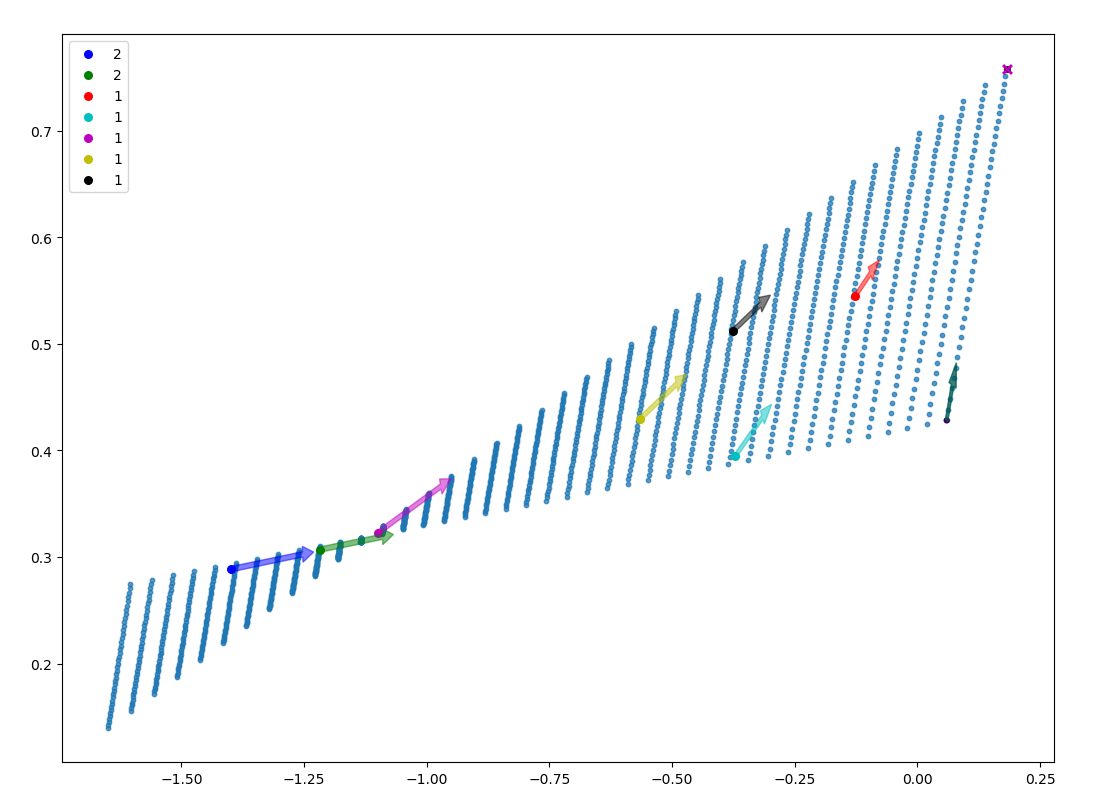
\includegraphics[width=0.8\textwidth,height=0.4\textheight]{../../pictures/figures/pi-polytope.png}
\caption{PI jumps between the deterministic policies (the vertices of our polytope).
This is because of the greedy step taken.}
\end{figure}

\newpage

\subsubsection{Policy gradients}

This search is closely related to the deep learning / end-to-end paradigm.
\textit{Simply write down what you want (the loss function),
estimate its derivative and apply gradient descent.}

In our case, the loss function is the value. And, we can estimate the derivative
by differentiating the value functional \ref{eq:value-functional} with respect to the policy.

To ensure the optimisation problem is constrained properly, we pick $\theta$ as our parameters and
construct the policy using $\pi = \sigma(\theta)$, where $\sigma$ is the softmax function.

% However, has problems with sparse rewards / exploration (not considered in this setting).
% (but dont they all have problems with sparse rewards!?)

\begin{algorithm}
\caption{Policy gradients}
\begin{algorithmic}[1]

\Procedure{PG}{$P, r, \gamma, \eta$}
  \State $t=0, \quad\quad \theta_t = \log(\pi) \quad\quad \pi \sim \mathcal U(\Pi)$ \Comment{Init}
  \While{not converged}
    \State $\theta_{t+1} = \pi_t + \eta \nabla_{\theta} V(\sigma(\theta_t))$ \Comment{Gradient update}
    \State t += 1
  \EndWhile
  \State \algorithmicreturn{ $\sigma(\theta_t)$}
\EndProcedure

\end{algorithmic}
\end{algorithm}

Note that to mitigate stability issues, we also added weak regularisation
attempting to maximise the entropy of the policy. This forces the policies away
from the edges of the polytope, where the gradients are not defined ($\log(0) = \text{NaN}$).

\begin{figure}[h!]
\centering
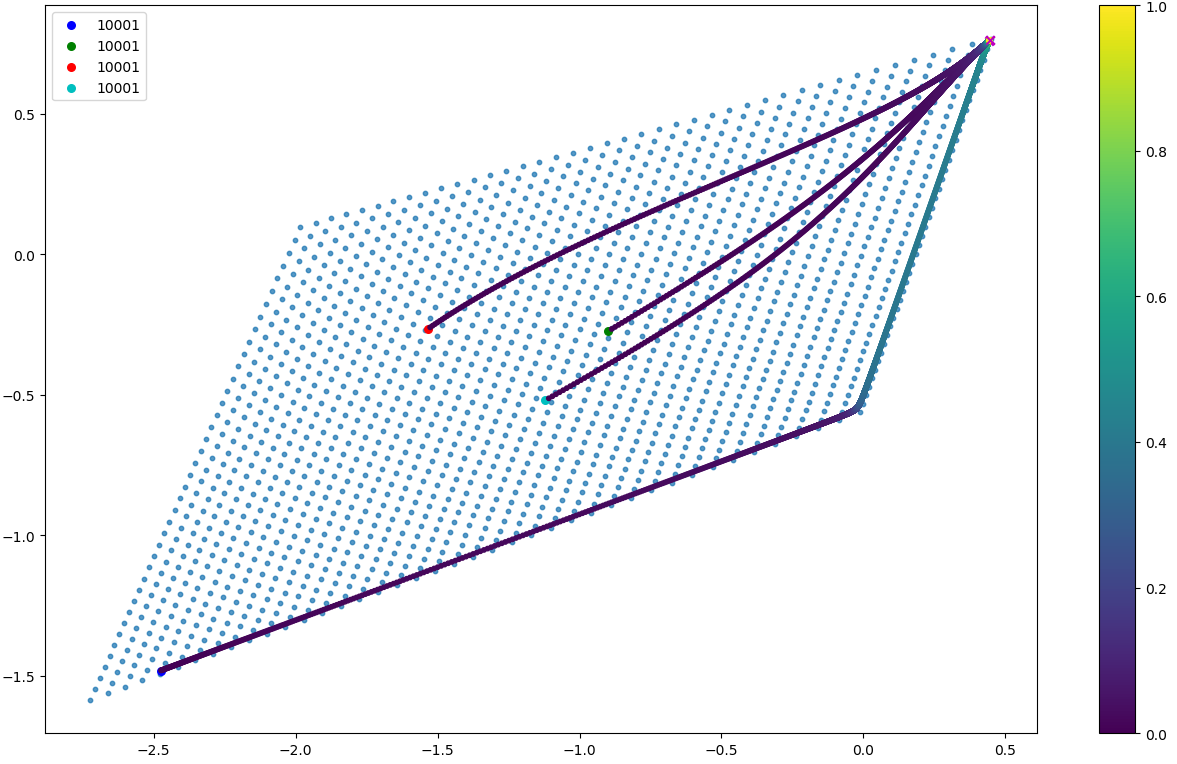
\includegraphics[width=0.8\textwidth,height=0.4\textheight]{../../pictures/figures/pg-polytope.png}
\caption{An example of ... . Note that the majority of }
\end{figure}

% Want to include upper / lower bounds!?
{\color{red}??? Converges at a rate of $\frac{1}{t}$. As can be seen by ...}
\cite{Agarwal2019a}.

\newpage

\subsection{Value search}

Alternatively, we can search through possible values. But how can we ensure that our search will
converge to a value that corresponds to a realisable policy? We can use Bellman's
optimality operator to guide the search.

(For similar reasons to why policy iteration converges) The greedy step using the
state-action values will find actions with higher value.


% (need to explain? why does stationarity mean optimality...?!)
Intution about why it converges!? Contraction. Banach fixed-point theorem.

% \begin{align}
% T(V) &= \mathop{\text{max}}_a \big[r + \gamma PV\big] \\
% \end{align}

\begin{algorithm}
\caption{Value iteration}
\begin{algorithmic}[1]

\Procedure{VI}{$P, r, \gamma, \eta$}
  \State t = 0
  \State $V_t = V(\pi) ; \;\; \pi \sim \mathcal U(\Pi)$ \Comment{Init}
  \While{not converged}
    % \State $V = r + \gamma PV_t$ \Comment{Evaluate}
    \State $Q = r + \gamma PV_t$ \Comment{Bellman operator}
    \State $\hat V = \text{max}_a Q(s, a)$
    \State $V_{t+1} = V_t + \eta (\hat V - V_t)$ \Comment{Average}
    \State t += 1
  \EndWhile
  \State $\pi = \mathop{\text{argmax}}_{\pi} r_{\pi} + \gamma P_{\pi}V_t$
  \State \algorithmicreturn{ $\pi$}
\EndProcedure

\end{algorithmic}
\end{algorithm}

\begin{figure}[h!]
\centering
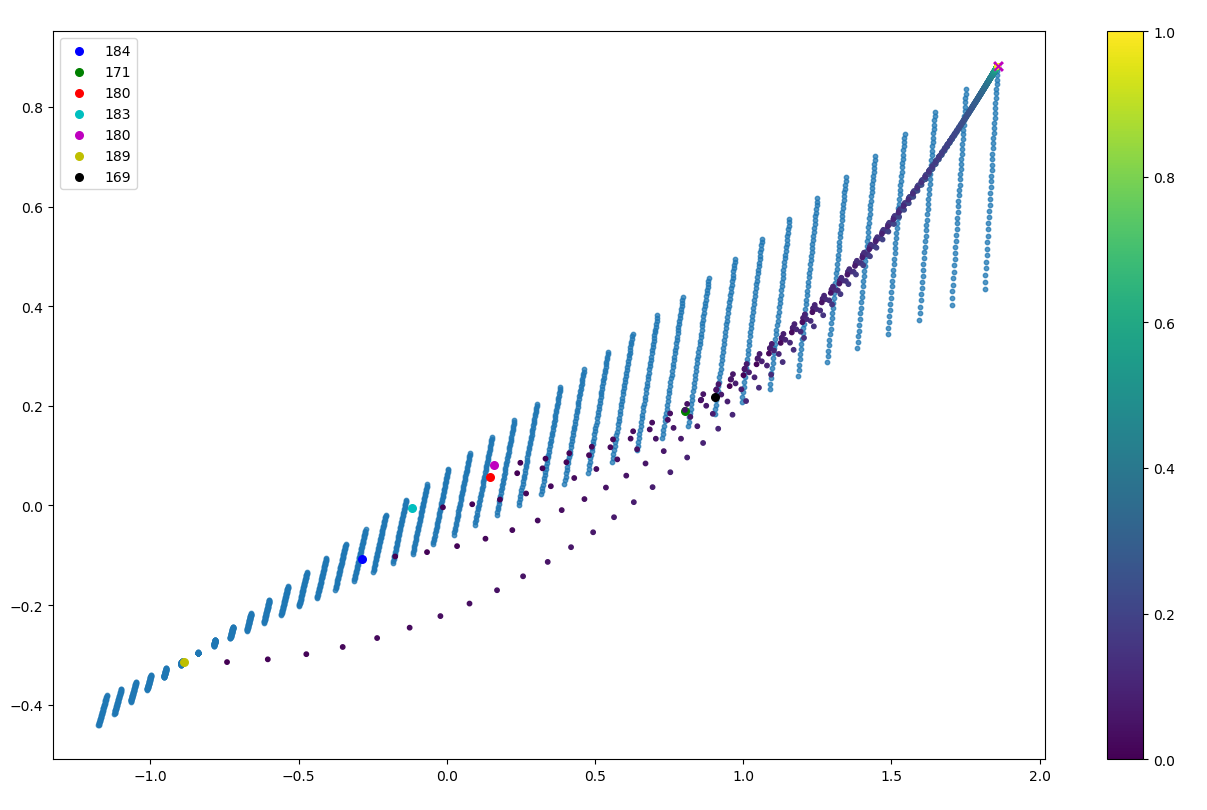
\includegraphics[width=0.8\textwidth,height=0.4\textheight]{../../pictures/figures/vi-polytope.png}
\caption{Observe that the value iterations are not constrained to map to a policy
(they can go out side of the polytope), but they do converge to a realisable policy,
the optimal one.}
\end{figure}

{\color{red}important. Also, why does it go outside?!?}
% Want to include upper / lower bounds!? On complexity. Sample / computational!?

\newpage

\begin{center}\rule{0.5\linewidth}{\linethickness}\end{center}

So there are different classes of search space: each imbued with special
structure from the Bellman equation or expected return. Each with different types of search they
support.

\begin{displayquote}
\textit{Which spaces support efficient search for the optimal policy? Can we characterise the properties of each space?}
\end{displayquote}

See appendix \ref{ss-extras} for an experimental exploration of the iteration complexity and dynamics of these different alforithms.
{\color{red}want to include in main section. but needs more work. not really sure what i am trying to say...}


\chapter{Abstraction}\label{C:bin}


\hypertarget{solveable-representations}{%
\section{Solveable representations}\label{solveable-representations}}

\begin{quote}
Representations with structure that is easily solvable.
\end{quote}

While there are other ways to add exploitable structure, here we only
consider linearity.

The bellman equation is a non-linear optimisation problem. It does have
some nice properties, like having a unique optima under the bellman
operator. But, in general, it isn't very friendly. Is there a way to
turn this into a linear problem? What sacrifices need to be made to
achieve this?

\hypertarget{why-linearity}{%
\subsubsection{Why linearity?}\label{why-linearity}}

\begin{itemize}
\tightlist
\item
  it has many mathematical tools for analysis.
\item
  we know linear systems can be solved efficiently.
\item
  ?
\end{itemize}

Linearity is a nice property that makes optimisation simpler and more
efficient.

\begin{itemize}
\tightlist
\item
  Linear programming (see appendix: LP)
\item
  Linear markov decision processes
\end{itemize}

Solving a system of linear relationships. Has a complexity of ???.

In fact. MDPs can actually be solved via LP. see {[}appendix{]}.

\hypertarget{a-closer-look-at-lmdps}{%
\subsubsection{A closer look at LMDPs}\label{a-closer-look-at-lmdps}}

(the Todorov ones\ldots{})

The three steps of abstraction - relaxation (transform to a new domain)
- linearisation (and solve) -

\hypertarget{lmdps-more-formally}{%
\paragraph{LMDPs; more formally}\label{lmdps-more-formally}}

\begin{figure}
\centering
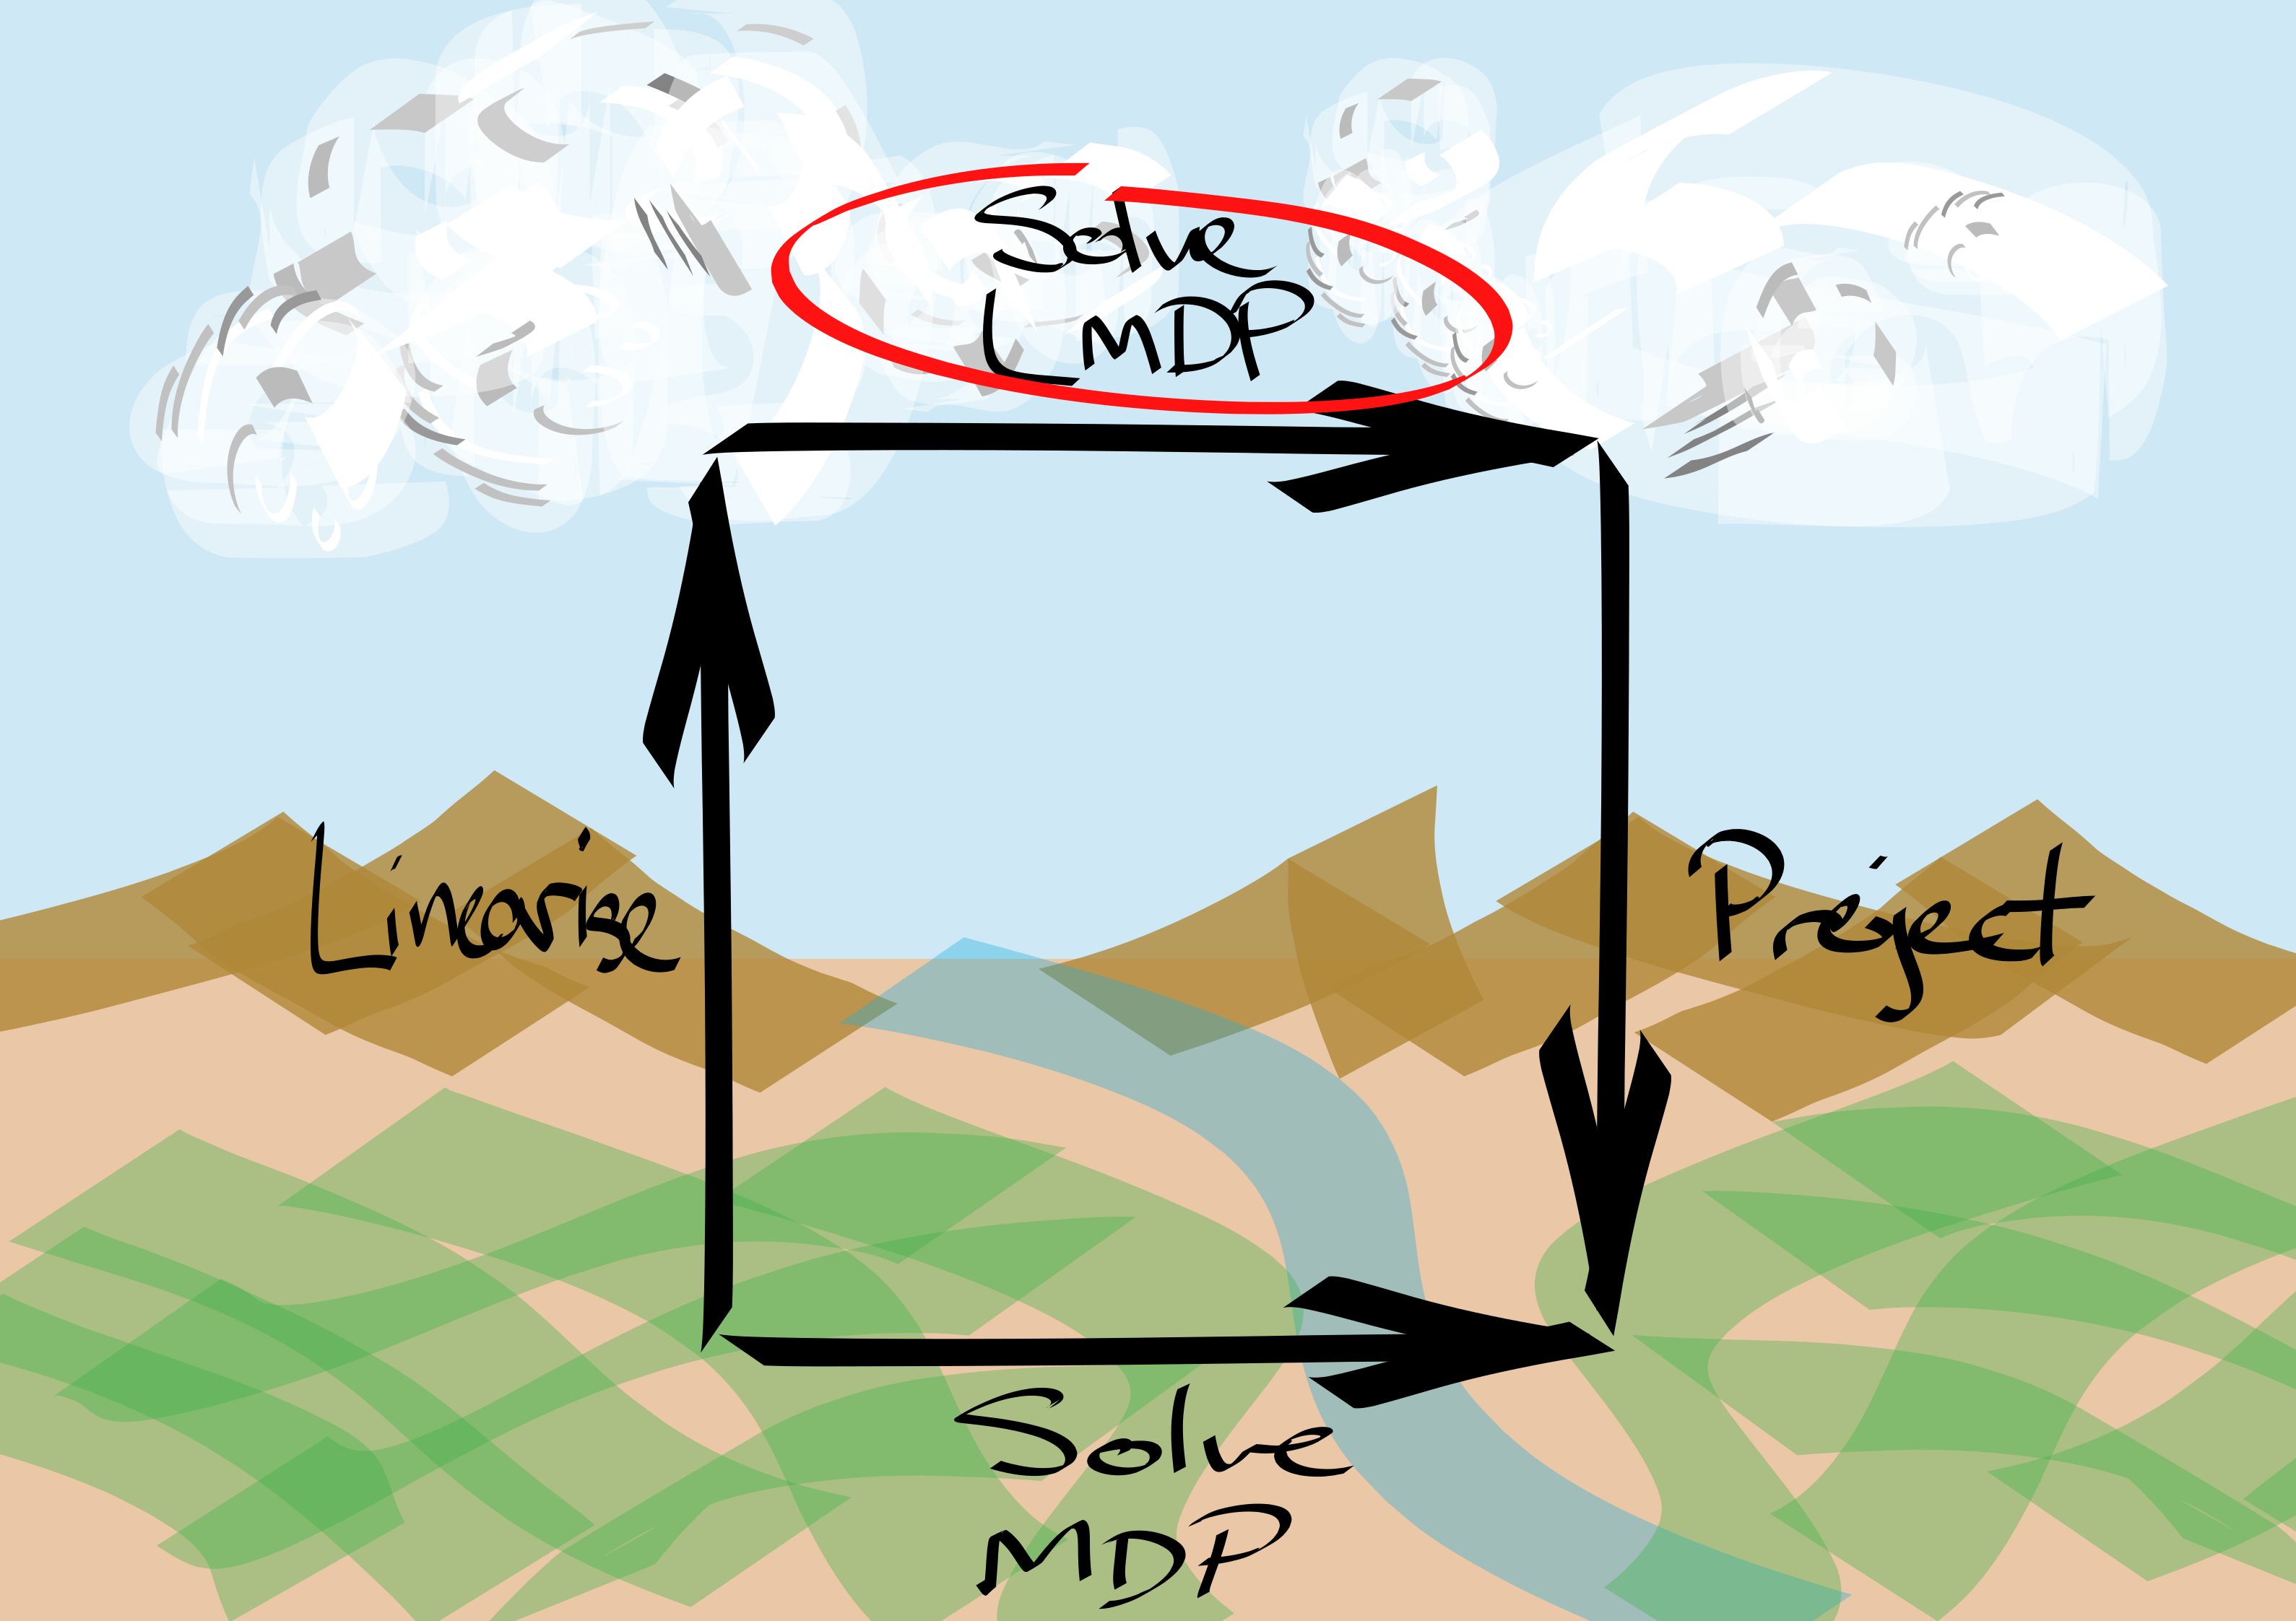
\includegraphics[width=0.5\textwidth,height=0.5\textheight]{../../pictures/drawings/abstract-representations-solve.png}
\caption{''}
\end{figure}

Pick \(a \in A\), versus, pick \(\Delta(S)\). \(f: S\to A\) vs
\(f:S \to \Delta(S)\).

In the original Todorov paper, they derive the LMDP equations for
minimising a cost function. This maximisation derivation just changes a
few negative signs around. Although there is also a change in the
interpretation of what the unconstrained dynamics are doing. \ldots{}?

\begin{align}
V(s) &= \mathop{\text{max}}_{u} q(s) - \text{KL}(u(\cdot| s) \parallel p(\cdot | s)) + \gamma \mathop{\mathbb E}_{s' \sim u(\cdot | s)} V(s') \tag{1}\\
\\
u^{* }(\cdot | s) &= \frac{p(\cdot | s)\cdot z(\cdot)^{\gamma}}{\sum_{s'} p(s' | s) z(s')^{\gamma}} \tag{8}\\
z_{u^{* }} &= e^{q(s)}\cdot P z_{u^{* }}^{\gamma} \tag{11}\\
\end{align}

By definition, an LMDP is the optimisation problem in (1). (3) Define a
new variable, \(z(s) = e^{v(s)}\). (5) Define a new variable that will
be used to normalise \(p(s' | s)z(s')^{\gamma}\). (8) Set the optimal
policy to minimise the KL distance term. (9) Since we picked the optimal
control to be the form in (8), the KL divergence term is zero. (11)
Rewrite the equations for the tabular setting, giving a \(z\) vector,
uncontrolled dynamics matrix.

(see appendix {[}{]} for a full derivation)

\hypertarget{a-relaxed-mdp}{%
\paragraph{A relaxed MDP}\label{a-relaxed-mdp}}

\begin{figure}
\centering
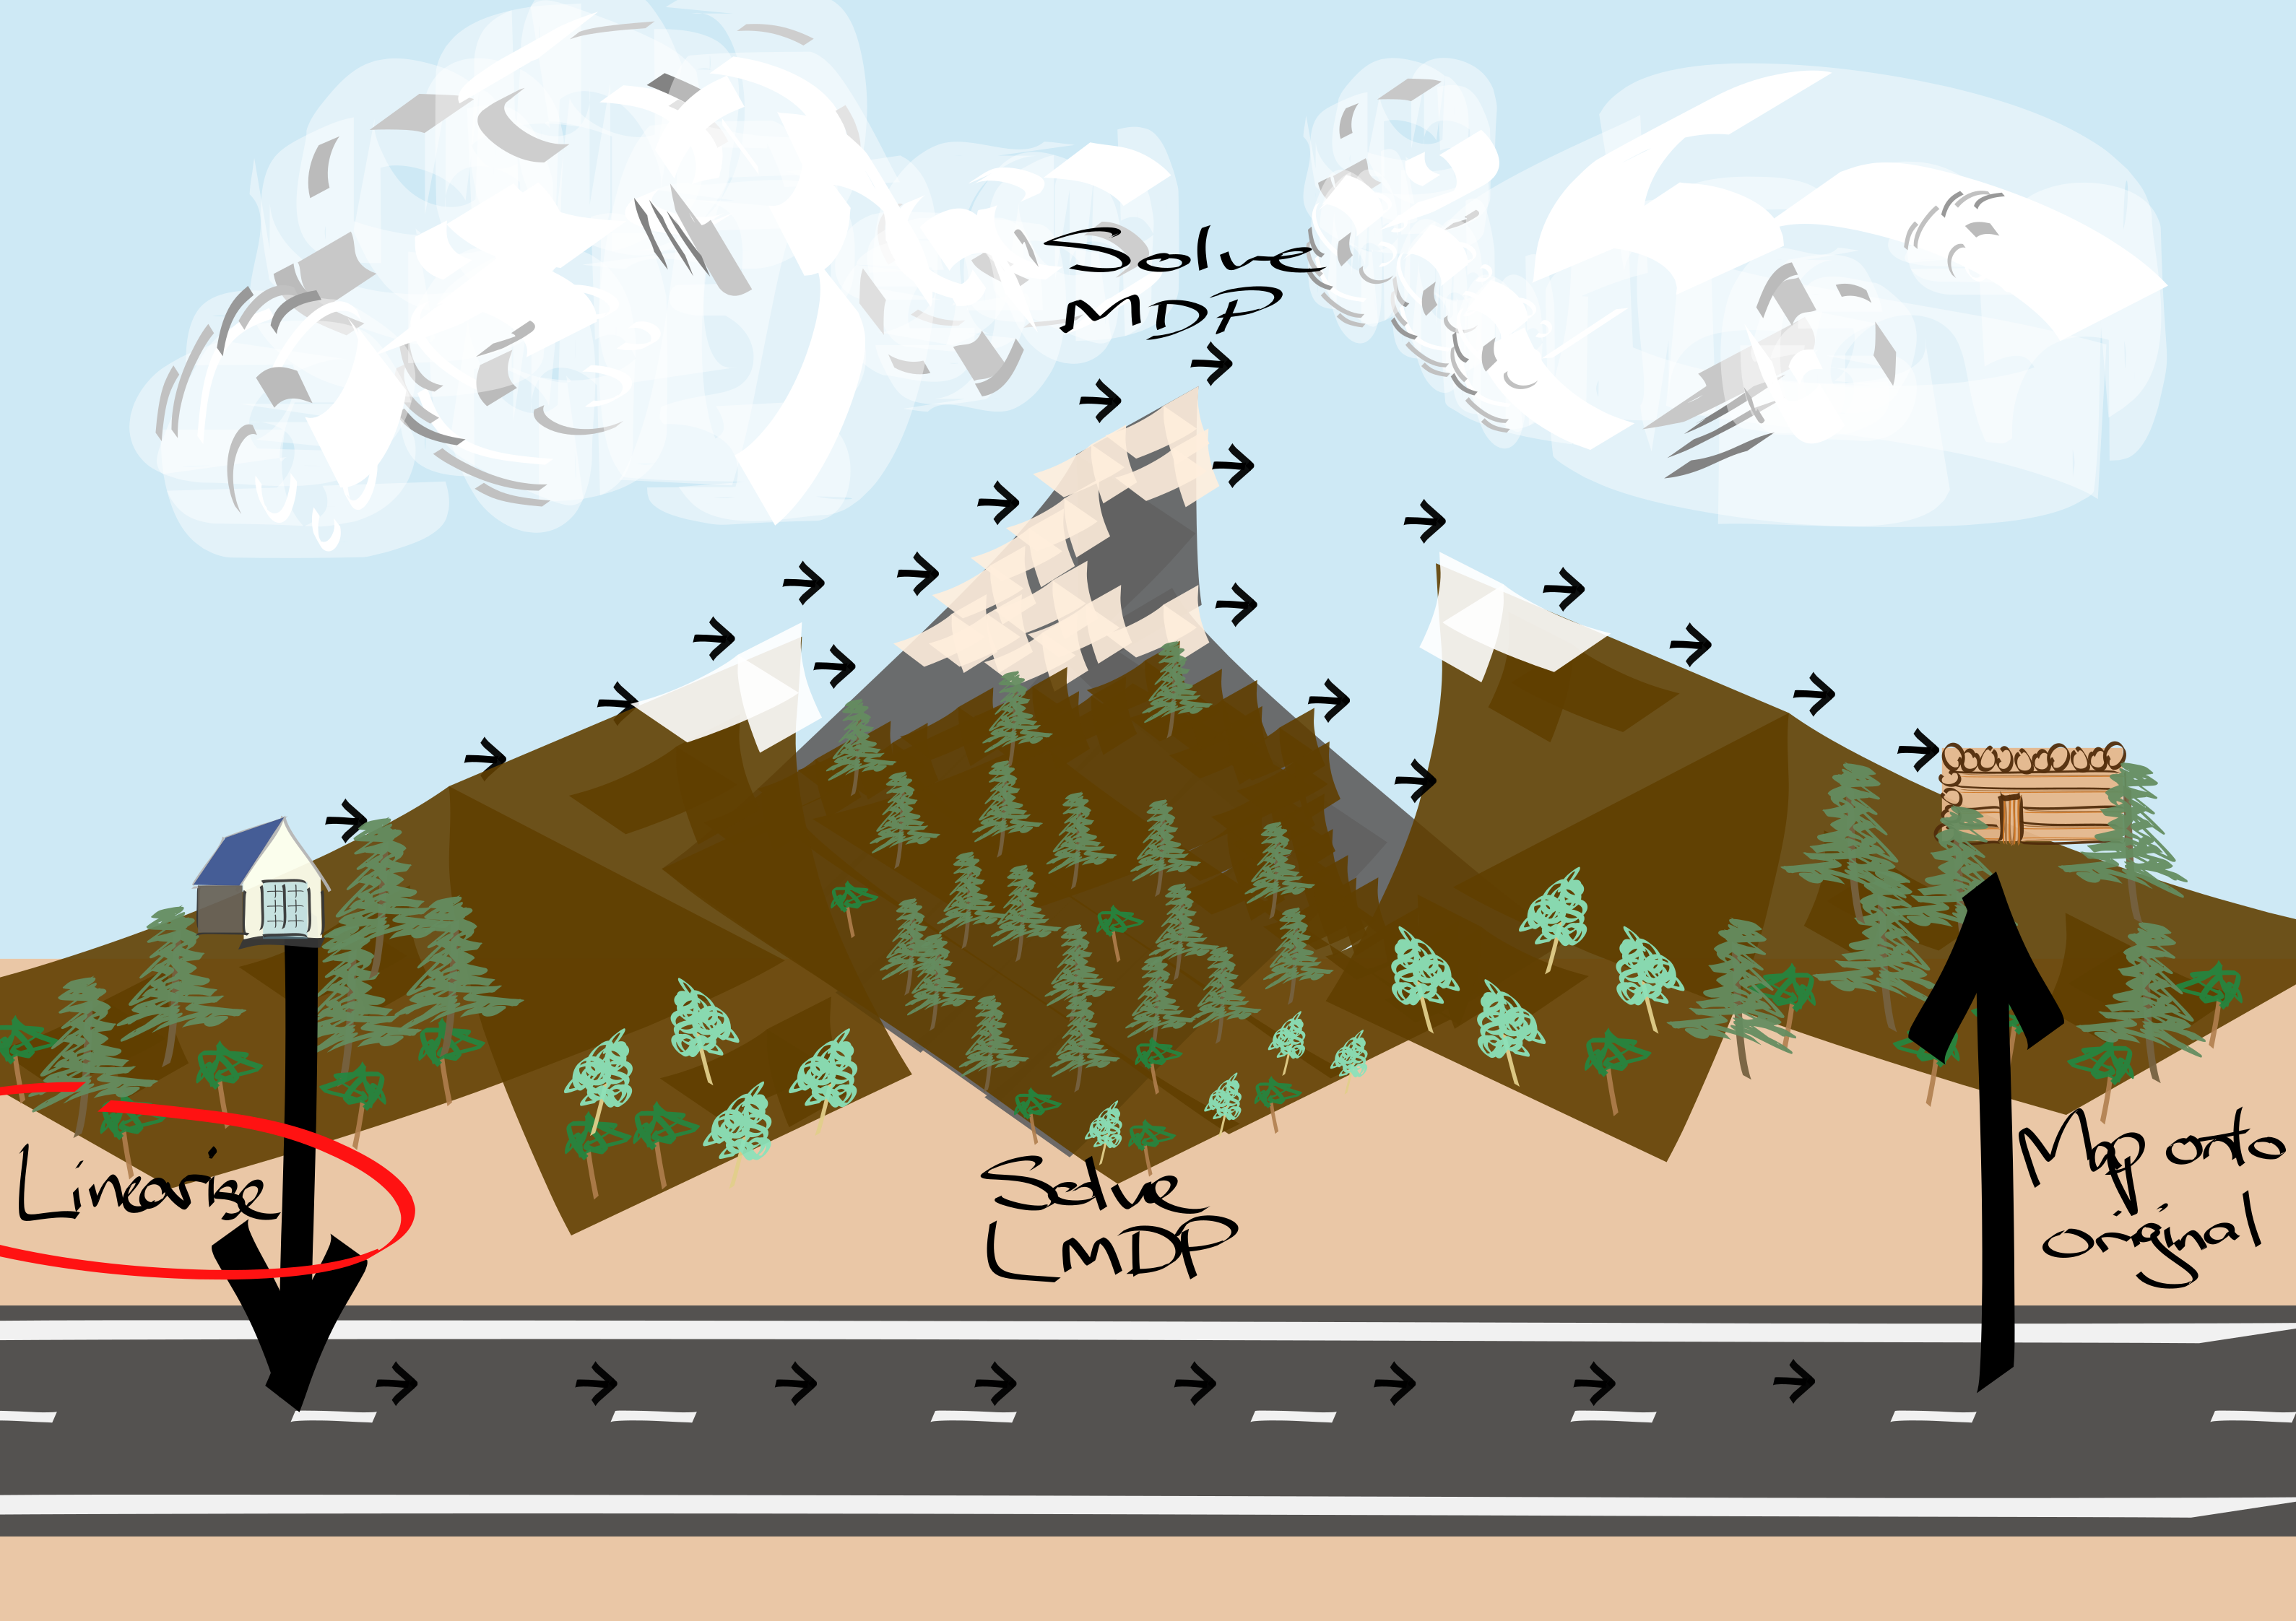
\includegraphics[width=0.5\textwidth,height=0.5\textheight]{../../pictures/drawings/abstract-representations-linear.png}
\caption{''}
\end{figure}

\begin{quote}
Ok great, we can solve LMDPs. But how does being able to solve an LMDP
help us solve MDPs?
\end{quote}

We want a way to transform a MDP into a LMDP, while preserving the
`structure' of the MDP. But what do we mean by a MDP's structure?

The LMDP, \(\{S, p, q, \gamma\}\) should;

\begin{itemize}
\tightlist
\item
  be able to represent the same transition dynamics as the original MDP,
\item
  give the the same rewards was the original MDP,
\item
  have the same optima.
\end{itemize}

(It turns out that (1) and (2) imply (3) given some assumptions. See
\href{}{Optimality})

So, given a reward function, \(r\), and a transition function, \(P\),
from the MDP, we must translate them into a \(p\) and a \(q\). Thus we
have built a LMDP with the same `structure'.

\begin{align}
\forall s, s' \in S, \forall a \in A, \exists u_a& \;\;\text{such that;} \\
P(s' | s, a) &= u_a(s'|s)p(s'|s) \tag{1}\\
r(s, a) &= q(s) - \text{KL}(P(\cdot | s, a) \parallel u_a(\cdot| s) ) \tag{2}\\
\end{align}

Which leads to \(|A|\) linear equations to solve, for each state in the
MDP.

See appendix {[}{]} for more details.

Alternative views of linearisation.

\begin{itemize}
\tightlist
\item
  A relaxation of the MDP
\item
  Linelihood interpretation
\end{itemize}

\hypertarget{unconstrained-dynamics-and-state-rewards}{%
\subparagraph{Unconstrained dynamics and state
rewards}\label{unconstrained-dynamics-and-state-rewards}}

\begin{quote}
Let's try and understand this thing we have contructed.
\end{quote}

The state rewards are not capable of giving rewards for actions taken.
Rather, the differences in reward, by taking another action, is captured
by the KL divergence between the control and the unconstrained dynamics.

\begin{itemize}
\tightlist
\item
  What is their function?
\item
  What do they look like?
\end{itemize}

Does it make sense to treat the q(s) like rewards?! They reward for bing
in state s. But cant capture action specific rewards!?

\hypertarget{decoding}{%
\paragraph{Decoding}\label{decoding}}

\begin{figure}
\centering
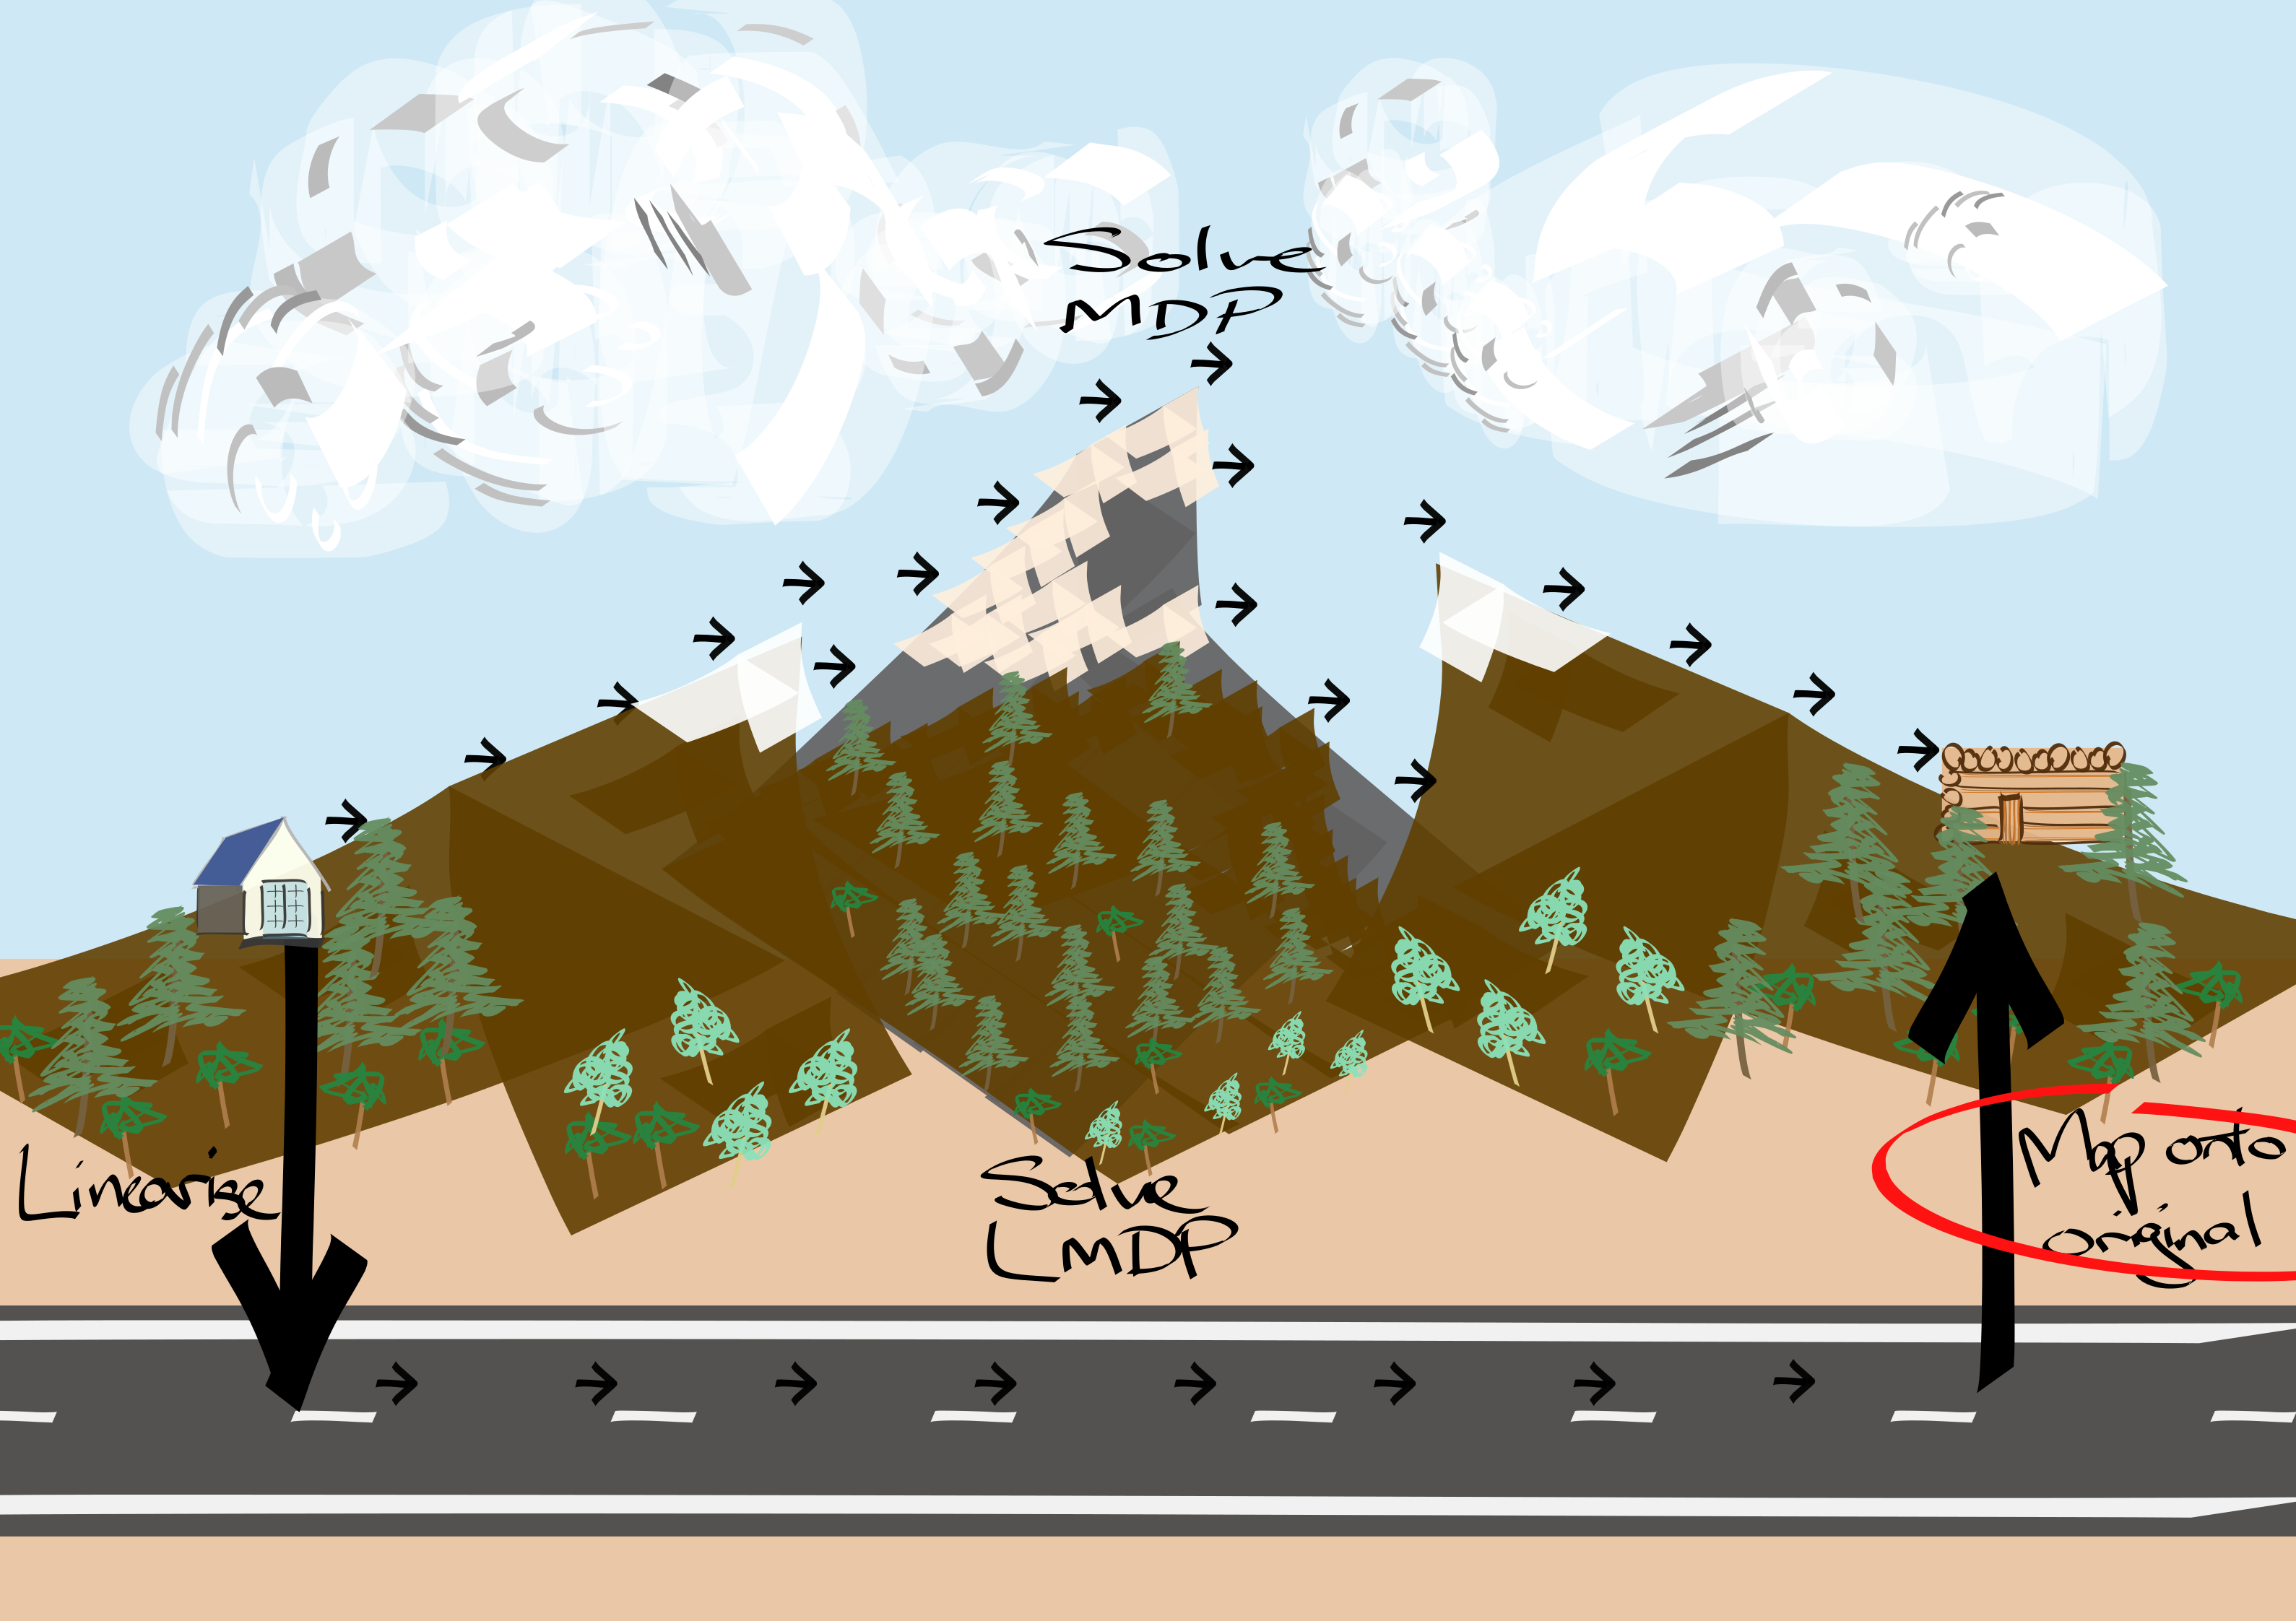
\includegraphics[width=0.5\textwidth,height=0.5\textheight]{../../pictures/drawings/abstract-representations-project.png}
\caption{''}
\end{figure}

Ok, so now we get a glimpse at why LMDPs are an interesting abstraction.
THe LMDP has disentangled the search for the behaviour (go to this or
that state) and the search for optimal controls (how to actually achieve
that behaviour). This can be seen in the decoding step. As we know which
states we want to be in, via the optimal control from solving the LMDP,
\(u^{* }\), but, we do not know how to implement those controls using
the actions we have available.

\begin{quote}
Two `simpler' problems. Easier to solve?
\end{quote}

\begin{align}
P_{\pi}(\cdot | s) = \sum_a P(\cdot | s, a) \pi(a | s) \\
\pi = \mathop{\text{argmin}}_{\pi} \text{KL}\Big(u(\cdot | s))\parallel P_{\pi}(\cdot | s)\Big)
\end{align}

Maybe this isnt enough? Do we need to add a reward sensitive part as
well?!? (but what if the actual path we take to get there has a neg
rewards?!?)

\hypertarget{optimality-of-solutions-via-lmdps}{%
\paragraph{Optimality of solutions via
LMDPs}\label{optimality-of-solutions-via-lmdps}}

\begin{quote}
Do these two paths lead to the same place?
\end{quote}

One of the main questions we have not addressed yet is; if we solve the
MDP directly, or linearise, solve and project, do we end up in the same
place? This is a question about the completeness of our abstraction. Can
our abstraction represent (and find) the same solutions that the
original can?

\begin{align}
\parallel V_{\pi^{* }} - \parallel V_{\pi^{* }} - V_{\pi_{u^{* }}} \parallel_{\infty}&= \epsilon  \tag{1}\\
&=\parallel (I - \gamma P_{\pi^{* }})^{-1}r_{\pi^{* }} - (I - \gamma P_{\pi_{u^{* }}})^{-1}r_{\pi_{u^{* } }} \parallel_{\infty} \tag{2}\\
&\le\parallel (I - \gamma P_{\pi^{* }})^{-1}r - (I - \gamma P_{\pi_{u^{* }}})^{-1}r \parallel_{\infty} \tag{3}\\
&=\parallel \bigg((I - \gamma P_{\pi^{* }})^{-1} - (I - \gamma P_{\pi_{u^{* }}})^{-1} \bigg) r \parallel_{\infty} \tag{4}\\
&\le r_{\text{max}} \parallel (I - \gamma P_{\pi^{* }})^{-1} - (I - \gamma P_{\pi_{u^{* }}})^{-1}   \parallel_{\infty} \tag{5}\\
&= r_{\text{max}} \parallel \sum_{t=0}^{\infty} \gamma^t P_{\pi^{* }} - \sum_{t=0}^{\infty} \gamma^t P_{\pi_{u^{* }}}  \parallel_{\infty} \tag{6}\\
&= r_{\text{max}} \parallel \sum_{t=0}^{\infty} \gamma^t (P_{\pi^{* }} - P_{\pi_{u^{* }}})   \parallel_{\infty} \tag{7}\\
&= \frac{r_{\text{max}}}{1-\gamma} \parallel P_{\pi^{* }} - P_{\pi_{u^{* }}} \parallel_{\infty} \tag{7}\\
\end{align}

\begin{enumerate}
\def\labelenumi{(\arabic{enumi})}
\tightlist
\item
  We want to compare the optimal policies value and the value achieved
  by the optimal LDMP solution.
\item
  Assume that there exists a policy that can generate the optimal
  control dynamics (as given by the LMDP). In that case we can set
  \(P_{\pi_{u^{* }}} = U^{* }\).
\item
  \(r_{u^{* }}\) doesnt really make sense as the reward is action
  dependent. We could calculate it as \(r_{\pi_{u^{* } }}\), but we dont
  explicity know \(\pi_{u^{* }}\). \((I - \gamma P_{\pi^{* }})^{-1}r\)
  represents the action-values, or \(Q\) values. By doing this exhange,
  we might over estimate the diffference under the infinity norm as two
  non-optimal actions may have larger difference. Also, use the element
  wise infinity norm.
\end{enumerate}

\begin{center}\rule{0.5\linewidth}{\linethickness}\end{center}

Ok, great. Insights from optimality bounds.

Need to be able to approximate the optimal controls. When is it hard to
approximate the optimal controls? When our basis set of distributions
oer future states (aka our actions) have little weight\ldots{}?

Potential solution? Use options.

\hypertarget{option-decoding}{%
\paragraph{Option decoding}\label{option-decoding}}

What about using options to help solve the optimal control decoding?
Does this actually help?!

\begin{align}
P_{\pi}(\cdot | s) = \sum_\omega P_k(\cdot | s, \omega) \pi(\omega | s) \\
\pi = \mathop{\text{argmin}}_{\pi} \text{KL}\Big(u(\cdot | s))\parallel P_{\pi}(\cdot | s)\Big)
\end{align}

Options would allow greater flexibility in the \(P_{\pi}(\cdot | s)\)
distribution, making is possible to match \(u(s'|s)\) with greater
accuracy (and possibly cost).

\begin{itemize}
\tightlist
\item
  First need to demonstrate that action decoding is lossy.
\item
  Then show that using options is less lossy.
\end{itemize}

This introduces dangers?!? As an option might accumulate unknown rewards
along the way!??

\hypertarget{the-complexity-of-solutions-via-lmdps}{%
\subsubsection{The complexity of solutions via
LMDPs}\label{the-complexity-of-solutions-via-lmdps}}

\begin{quote}
Is my path actually shorter?
\end{quote}

The whole point of this abstraction was to make the problem easier to
solve. So hasit actually made it any easier?

The complexity of solving our abstraction can be broken down into the
three steps;

\begin{itemize}
\tightlist
\item
  linearisation: \(|S| \times \text{min}(|S|,|A|)^{2.3}\)
\item
  solve the LMDP: \(\text{min}(|S|,|A|)^{2.3}\)
\item
  project back: \(???\)
\end{itemize}

Giving a total complexity of \ldots{}

Contrasted with the complexity of solving an MDP.

\hypertarget{scaling-to-more-complex-problems}{%
\subsubsection{Scaling to more complex
problems}\label{scaling-to-more-complex-problems}}

Now that we have some evidence that this LMDP solution strategy makes
sense, it efficiently (see \href{}{complexity}) yields high value (see
\href{}{optimality}) policies. We want to test it out on some real world
problems. But the real world isn't as nice as the setting we have been
working in. There are a few added complexities;

\begin{itemize}
\tightlist
\item
  sample based / incremental
\item
  large / cts state spaces
\item
  sparse rewards
\end{itemize}

So now that we have explored LMDPs, how can we extract their nice
properties into an architecture that might scale to more complex
problems: larger state spaces and action spaces, sparse rewards,
\ldots{}?

\hypertarget{incremental-implementation}{%
\paragraph{Incremental
implementation}\label{incremental-implementation}}

Generalise to a more complex problem. We are only given samples. A first
step to tackling more complex problems.

\hypertarget{model-based}{%
\subparagraph{Model based}\label{model-based}}

Learn \(p, q\) based on samples.

\begin{align}
\mathcal L(\theta, \phi) = \mathop{\mathbb E}_{s, a,} \bigg[ r(s, a) - q_\theta(s) + \text{KL}(p_\phi(\cdot | s) \parallel P(\cdot | s, a)) \bigg]\\
\mathcal L(\theta, \phi) = \mathop{\mathbb E}_{s, r, s'} \bigg[r - q_\theta(s) - p_\phi(s' | s) \log \frac{1}{ p_\phi(s' | s)} \bigg] \\
\end{align}

\begin{center}\rule{0.5\linewidth}{\linethickness}\end{center}

Ok. Lets take a different approach. \textbf{Q:} Why is it a bad idea to
try to do incremental RL with this linearisation trick? Not sure.

\begin{center}\rule{0.5\linewidth}{\linethickness}\end{center}

Alternative perspective. The high value trajectories are the most likely
ones.

\hypertarget{distributions-over-states}{%
\subsubsection{Distributions over
states}\label{distributions-over-states}}

What if we wanted to approximate these distributions? Generalise subgoal
methods to work with distributions? The distribution could be
constructed via; parzen window / GMM, neural flow, ?!.

Connections to distributional RL?

Questions

\begin{itemize}
\tightlist
\item
  What is p(s'\textbar{}s)!?!?
\item
  Want some examples of MDPs they cannot solve.
\item
  What is the relationship to other action embedding strategies?
\item
  How does p(s'\textbar{}s) bias the controls found??? I can imagine the
  unconstrained dynamics acting as a prior and prefering some controls
  over others.
\item
  If we have m states and n actions. Where m
  \textgreater{}\textgreater{} n. Then \(u(s'|s)\) is much larger than
  \(\pi(a|s)\). Also, \(u(s'|s)\) should be low rank?!
  \(u_{s's} = \sum_a u_a \alpha_a u_a^T\)
\end{itemize}

\hypertarget{other-properties}{%
\subsection{Other properties}\label{other-properties}}

LMDPs have the property that if we have already solved two LMDPs, with
the same state space, action space, unconditioned transition dynamics,
but different state rewards, \(q_1, q_2\). Then we can solve a new LMDP,
again with the same, \ldots{}, and state rewards in the span of
\(q_1, q_2\), \(z_3 = w_1 z_1 + w_2 z_2\), \ldots{}

Problem. What does it even mean for two LMDPs to have the same
unconditioned dynamics but different state rewards? The MDPs must have
been the same up to some additive constant (constant in the actions),
\(r(s, a)=r(s, a) + c(s)\). Does this really capture what we mean by
different tasks?!?

AND HRL!?!?

Refs \cite{Todorov2006,Todorov2009,Zhong,Zhonga,Dvijotham,Wozabal}

\hypertarget{near-optimal-abstractions}{%
\section{Near optimal abstractions}\label{near-optimal-abstractions}}


We are working with MDPs \((S, A, \tau, r)\), therefore we have a state
space, \(S\), an action space, \(A\), a transition function
\(P: S\times A \times S \to [0, 1]\) and a reward function
\(r: S\times A \to \mathbb R\).

Let's say we have an abstraction, (a road is a road, no real different
between them), a natural thing we want to know about the abstraction is:
is it possible for me to act optimally using this abstraction, if not,
what's the damage (in this case, of driving 100kph on every road,
because they are all prety much the same\ldots{})? Or, in other words,
which policies are approximately representable within this abstracted
MDP.

An abstract MDP is defined as;

???

The metric we are optimising is the representation error of the optimal
policy. Given an abstraction, we want to know how well the abstraction
can represent the optimal policy.

\[
\forall_{s\in S_G, a\in A_G} \mid Q_G^{\pi^* }(s, a) - Q_G^{\pi_{GA}^* }(s, a) \mid \le 2 \epsilon \eta_f
\]

We could impose properties on a state abstraction using something like
the following;


\begin{align}
\forall_{s_1, s_2 \in S} \mid f(s_1) - f(s_2)\mid \le \epsilon &\implies \phi (s_1) = \phi(s_2)\\
\forall_{\cdot} \mid f(\cdot) - f(\cdot)\mid \le \epsilon &\implies g_1(\cdot) = g_2(\cdot)\\
\end{align}


In other words, if there exists an approximate similarity, according to
\(f\), then build it into our abstraction.

\begin{itemize}
\tightlist
\item
  \textbf{Q:} How should we construct our abstraction?
\item
  \textbf{Q:} What properties should it have to achieve `good'
  performance?
\end{itemize}

Using the above method of imposing properties on an abstraction, what
should we pick as \(f\)?

\begin{enumerate}
\def\labelenumi{\arabic{enumi}.}
\tightlist
\item
  The policy function:
  \(\forall_{\cdot_a, \cdot_b \in D} \mid \pi(\cdot_a) - \pi(\cdot_b) \mid \le \epsilon\)
  is approximately the same.
\item
  The transition function:
  \(\forall_{\cdot_a, \cdot_b \in D} \mid \tau(\cdot_a) - \tau(\cdot_b)\mid \le \epsilon\)
  is approximately the same.
\item
  The reward function:
  \(\forall_{\cdot_a, \cdot_b \in D} \mid r(\cdot_a) - r(\cdot_b) \mid \le \epsilon\)
  is approximately the same.
\end{enumerate}

Also,

\begin{enumerate}
\def\labelenumi{\arabic{enumi}.}
\setcounter{enumi}{3}
\tightlist
\item
  The policy trajectory:
  \(\forall_{\cdot_a, \cdot_b \in D} \mid \sum_{t=0}^T \parallel \pi(\cdot_a) - \pi(\cdot_b)\parallel_1 \mid \le \epsilon\)
  is approximately the same.
\item
  The transition trajectory:
  \(\forall_{\cdot_a, \cdot_b \in D} \mid \sum_{t=0}^T\parallel \tau(\cdot_{a_t}) - \tau(\cdot_{b_t})\parallel_1\mid \le \epsilon\)
  is approximately the same.
\item
  The reward trajectory:
  \(\forall_{\cdot_a, \cdot_b \in D} \mid \sum_{t=0}^T \parallel r(\cdot_{a_t}) - r(\cdot_{b_t})\parallel_1 \mid \le \epsilon\)
  is approximately the same.
\end{enumerate}

GVFs

\begin{enumerate}
\def\labelenumi{\arabic{enumi}.}
\setcounter{enumi}{6}
\tightlist
\item
  The discounted future policy:
  \(\forall_{\cdot_a, \cdot_b \in D} \mid \Pi(\cdot_a) - \Pi(\cdot_b)\mid \le \epsilon\)
  is approximately the same.
\item
  The discounted future transition:
  \(\forall_{\cdot_a, \cdot_b \in D} \mid \Upsilon(\cdot_a) - \Upsilon (\cdot_b)\mid \le \epsilon\)
  is approximately the same.
\item
  The discounted future reward:
  \(\forall_{\cdot_a, \cdot_b \in D} \mid Q(\cdot_a) - Q(\cdot_b)\mid \le \epsilon\)
  is approximately the same.
\end{enumerate}

\textbf{Q:} Which is best?

\begin{quote}
\textbf{Claim 1:} 9.(the value fn) will yield the most compression,
while performing well. But, it is a task specific representation, thus
it will not transfer / generalise well.
\end{quote}

\hypertarget{other-types-of-abstraction}{%
\paragraph{Other types of
abstraction}\label{other-types-of-abstraction}}

We constructed the state abstraction by altering what the policy and
value function were allowed to see. Rather than observing the original
state space, we gave them access to an abstracted state space.

There are other ways to alter what the policy and value function sees.


\begin{align}
\phi: S \to X&: \quad \pi(s) \to \pi(\phi(s)) \quad Q(s, a) \to Q(\phi(s), a) \tag{State abstraction} \\
\psi: A\to Y&: \quad \pi(s) \to \psi^{-1}(\pi(s)) \quad Q(s, a) \to Q(s, \psi(a)) \tag{Action abstraction} \\
\phi, \psi&: \quad \pi(s) \to \psi^{-1}(\pi(\phi(s))) \quad Q(s, a) \to Q(\phi(s), \psi(a)) \tag{State and action abstraction} \\
\varphi: S \times A \to Z&: \quad \pi(s)\to \mathop{\text{argmax}}_a V(\varphi(s, a)) \quad\quad Q(s, a) \to V(\varphi(s, a)) \tag{State-action abstraction} \\
\end{align}


\begin{quote}
\textbf{Claim 2:} The state-action abstraction is the most powerful
because it allows the compression of the most symmetries. (want to
prove!)
\end{quote}

(relationship to
\href{http://www.gatsby.ucl.ac.uk/~dayan/papers/d93b.pdf}{Successor
features}!?)

State abstraction groups together states that are similar. For example,
sprinting 100m is equivalent regardless of which track lane you are in.

Action abstraction groups together actions that are similar. For
example, X and Y both yeild the state change in state, \textgreater{}
Approximation perspective: we have a set of options and we want to use
them to approximate the optimal policy. A good set of options can
efficiently achieve an accurate approximation.

\hypertarget{motivating-example-for-state-and-action-abstraction}{%
\subsubsection{Motivating example for state and action abstraction:
???}\label{motivating-example-for-state-and-action-abstraction}}

Might want to transfer. But some envs share state space, some share
action space. Want to

\begin{itemize}
\tightlist
\item
  Might be teleported to a new environment? (new state space, same
  action space)
\item
  Might have to drive a new vehicle (same state space, new action space)
\end{itemize}

\hypertarget{motivating-example-for-state-action-abstraction-symmetric-maze}{%
\subsubsection{Motivating example for state-action abstraction:
Symmetric
maze}\label{motivating-example-for-state-action-abstraction-symmetric-maze}}

\emph{(Some intuition behind claim 2.)}

Imagine you are in a mirror symmetric maze. It should not matter to you
which side of mirror you are on.

\begin{figure}
\centering
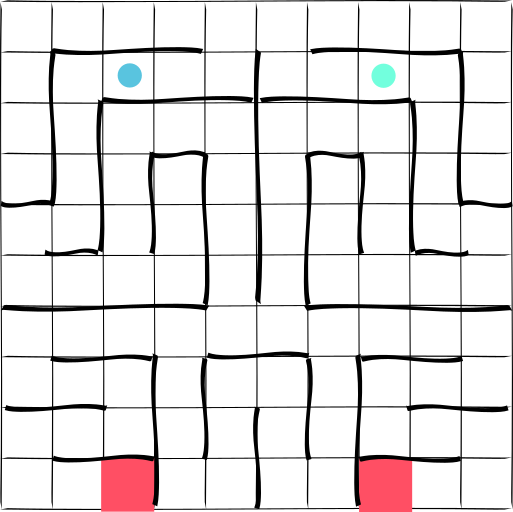
\includegraphics[width=0.5\textwidth,height=0.5\textheight]{../../pictures/drawings/maze.png}
\caption{maze.png}
\end{figure}

This reduces the state-action space by half!
\(\frac{1}{2}\mid S \mid \times \mid A \mid\). Note: just using state
abstraction it is not possible to achieve this reduction. Mirrored
states are not equivalent as the actions are inverted.

While other learners can still solve this problem. They miss out on
efficiency gains by abstracting first.

\hypertarget{related-work}{%
\subsubsection{Related work}\label{related-work}}

Other approaches to abstraction for RL focus on \ldots{}?

Near Optimal Behavior via Approximate State Abstraction \cite{Abel2017}
A Geometric Perspective on Optimal Representations for Reinforcement Learning \cite{Bellemare2019b}
successor representation

\hypertarget{discussion}{%
\subsection{Discussion}\label{discussion}}

But can we guarantee that these abstractions do not make it harder to
find the optimal policy? Is that even possible?

\begin{center}\rule{0.5\linewidth}{\linethickness}\end{center}

Want a general way (a function) to take an abstraction of an MDP
(defined by certain propreties) and return the difference between its
optimal policy and the true optimal policy. Want automated computational
complexity to solve this! Actually, we are not considering computational
complexity here only approximation error. For that can we just use
automatic differentiation!? Want a way to get bounds for all of these
combinations!

\begin{center}\rule{0.5\linewidth}{\linethickness}\end{center}

How do we know one policy is better than another? How do we know a
policy is optimal?

\[
\forall \pi\;\; V^{\pi^* } \ge V^{\pi} \\
\]

But, this definition of optimality implicitly assumes a uniform
distribution over states. This is unlikely. Rather, the distribution is
determined by the policy.

\[
\mathop{{\mathbb E}}_{s\sim D_{\pi}} \big[ V^{\pi^* } \big] \ge \mathop{{\mathbb E}}_{s\sim D_{\pi}} \big[ V^{\pi} \big] \\
D_{\pi}(s) = P(s | \pi) = \sum_{\text{all } \tau \text{ with } s_t = s} P(\tau | \pi)
\]

Now. How different is this?

I can imagine some degenerate solutions now being possible? Because we
can control the distribution we are being evaluated on. We could pick a
policy that oscillates between two states, never leaving the cycle.
Therefore it would have \(p(s_1) = p(s_2) = 0.5\) and
\(p(s_{i \neq 1,2}) = 0\).

That doesn't seem so bad?

\newpage
\section{Efficiently solvable abstractions}\label{solveable-abstractions}

\begin{displayquote}
  \textsl{Abstractions for efficient control.}
\end{displayquote}

% The control problem can be expensive, especially when there are long horizons, or high discount rates.
% For example, bound, bound. Can

In optimisation for supervised learning we know that
linear models can be solved analytically and convex problems converge quickly.
What makes an RL problem easy to solve? Is there linearity or convexity
within RL problems that we can use to find solutions more efficiently?

% bellman eqn is hard to solve (how hard?)
% Existing solvers of MDPs such as are not efficient: value iteration requires at
% least \href{https://en.wikipedia.org/wiki/EXPTIME}{EXPTIME} iterations,
% policy iteration requires ???, or policy gradients,
% require a ??? amount of computation.
% Yet, recent work \cite{} has shown that MDPs require at least $\Omega(|S|^2|A|).$

While some interesting work has been done exploring convex RL \cite{ODonoghue2012a, Barratt2019},
we choose to explore linear RL.

\subsection{Linear Markov decision problems (LMDPs)}

\begin{displayquote}
\textsl{Why linear MDPs?}
\end{displayquote}

% How are we exploiting linearity?
% Linearisation around the optima? Intuition. How to see this? Stephen!?
% Intuition.

% \subsubsection{Existing linear methods}
%
% The optimal policy of a MDPs can be found be using linear programming.
% Traversing through the (value ??) space, ...?

% many mathematical tools for analysis.
% we know linear systems can be solved efficiently.

% Linear systems are easy to solve. (ref). They have $\mathcal O(n^3)$ complexity.

Imagine if your life were linear, in the sense of effort and achieving goals.
More work equals proportionally more rewards. This makes decision making
a lot more simple. Pick the most rewarding activity, and work hard.

\subsubsection{What do we mean by a linear MDP?}

Do we mean that the value function is a linear function of (say) a policy?
Of the reward function? Of the transition function? Previous research has tried to incorporate
linearity into MDPs in a few different ways.

\begin{itemize}
  \tightlist
  \item Todorov constructs a linearised MDP that is linear in the 'control' (a proxy for the policy) \cite{Todorov2006}.
  \item Jin et al. construct a MDP where the value is a linear function of a state-action representation and of a policy embedding \cite{Wang}.
  \item Levine et al. construct a learner that assumes a linear transition function, allowing the use of \href{https://en.wikipedia.org/wiki/Linear%E2%80%93quadratic_regulator}{LQR} solvers \cite{Levine2019}.
  \item Pires et al. construct a factored linear MDP that allows the TD operator to be applied in a lower dimensional space \cite{Pires2016}.
\end{itemize}

Todorov's formulation appears to be the most powerful. By having a linear
relationship between the value and the control, we can easily search for controls that
are optimal. For the rest of this work we will refer to these as LMDPs.

% Saxe el al. observe the power of linearity: \textit{"Consider two standard MDPs
% $M_1 = \{S, A, P, R_1\}$ and $M_2 = \{S, A, P, R_2\}$ which have
% identical state spaces, action sets, and transition dynamics but differ in their
% instantaneous rewards $R_1$ and $R_2$. These may be solved independently to
% yield value functions $V_1$ and $V_2$. [If the problems were linear then] the value function of the MDP
% $M_{1+2} = \{S, A, P, R_1 +R_2\}$, whose instantaneous rewards are the sum of the
% first two, [would be] $V_{1+2} = V_1 + V_2$.} \cite{Saxea}

\subsubsection{Constructing a LMDP}

\begin{figure}[h!]
  \centering
  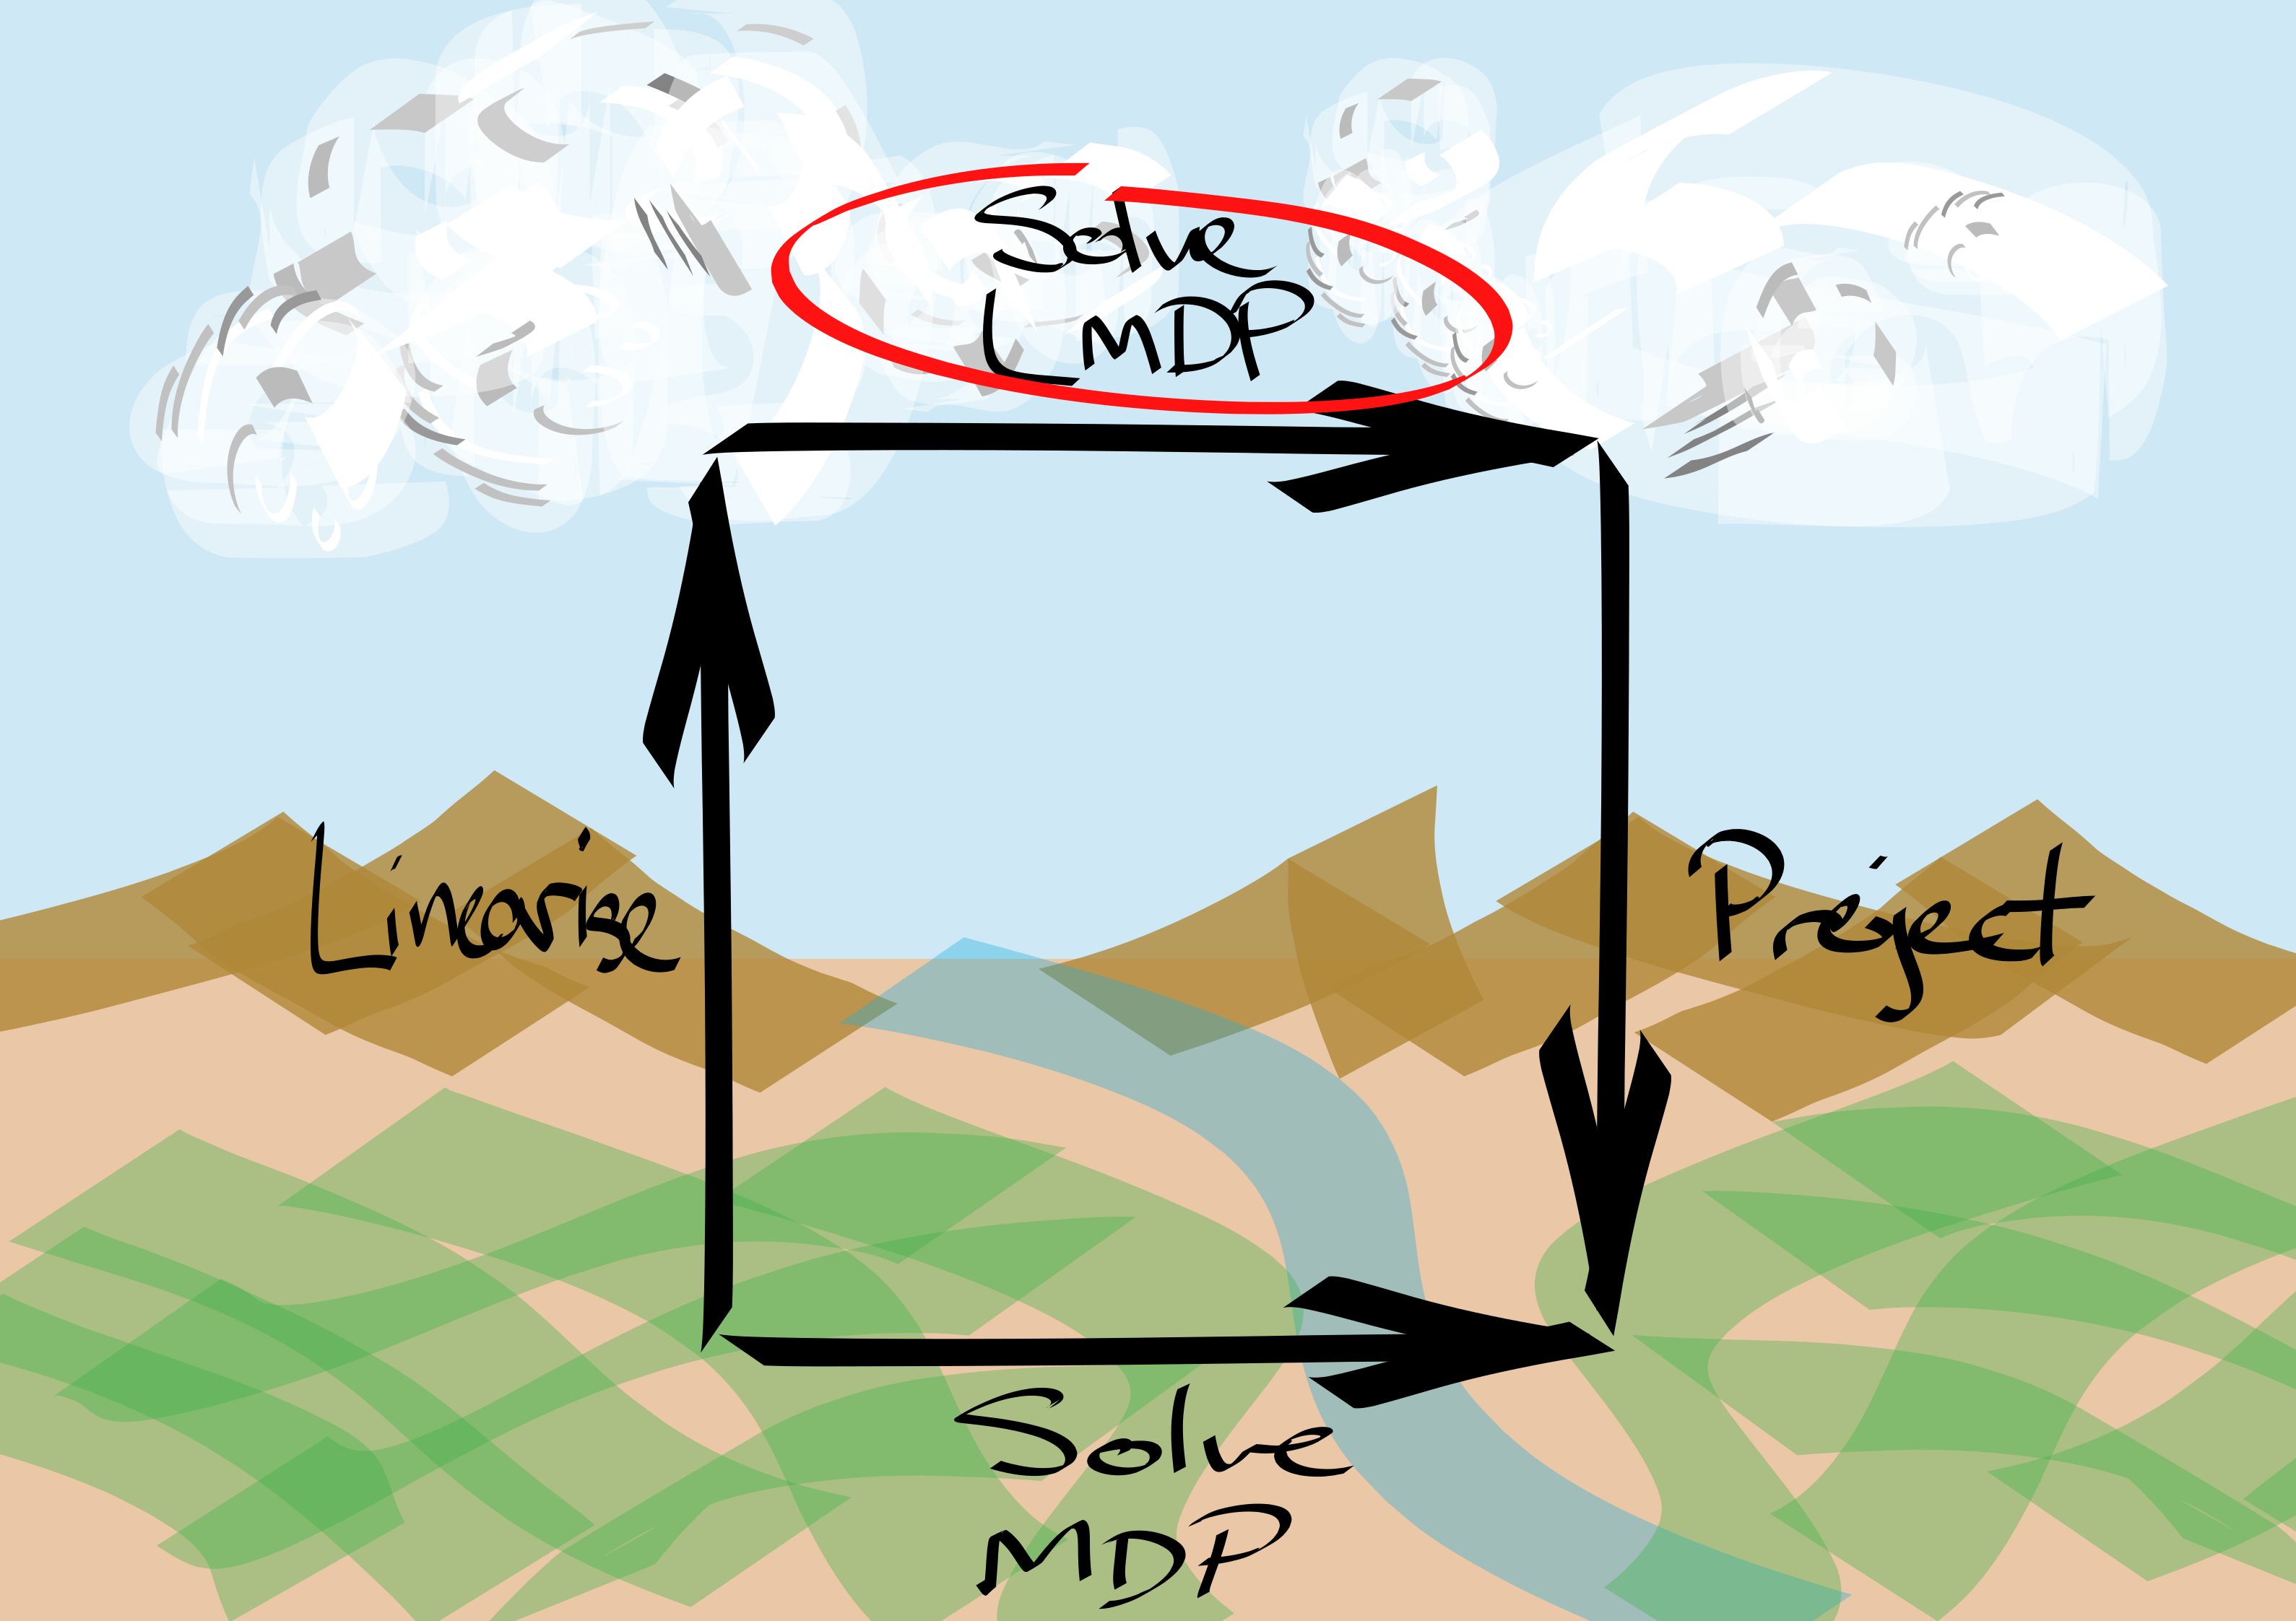
\includegraphics[width=0.6\textwidth,height=0.3\textheight]{../../pictures/drawings/abstract-representations-solve.png}
  \caption{Solving the LMDP}
\end{figure}

To build a LMDP that acts similarly to a MDP, Todorov \cite{Todorov2006} incorporate a few changes to the typical MDP setting;

\begin{itemize}
\tightlist
  \item
  allow the agent to pick actions in the space of possible transitions, which they name 'controls', $u: S \to S$.
  \item
  ensure that chosen controls are possible under the given transition function, a new reward is added.
  Controls are rewarded if they are close to the 'unconstrained dynamics', $p(s' | s)$.
  \item
  maximise the exponentiated cumulative rewards.
  $\mathop{\text{max}}_{u} \mathop{\mathbb E}_{\zeta \sim D(u)} e^{R(\zeta)}$ \cite{EricWarrenFox2016} (rather than maximizing the cumulative reward).
\end{itemize}

The intuition behind these changes seems to be; we have allowed the learner to pick an arbitrary control.
This simplifies the optimisation problem. But, now the learner might pick a control that is not possible
under the given transition function. So we incentivise controls that are close to the underlying dynamics.

\begin{displayquote}
\textit{"It is reminiscent of a linear programming relaxation in integer programming"} \cite{Todorov2009}.
\end{displayquote}

% What is the relationship to other action embedding strategies? {\color{red}!!!!!}

% Why did they need these tricks? Which ones were necessary / sufficient? !!!!!!!

% formal definition
Putting these changes together, a linear Markov decision process can be formulated as;
LMDP $=\{S, U, p, q, \gamma\}$. Where $S$ is the state space, $U$ is the space of possible controls (i.e. any transitions),
$p: S \to S$ is the unconditioned dynamics, and $q \in \mathbb R^{|S|}$ is state rewards.
Our goal is to find the control, $u: S \to S$, that gives the highest exponentiated cumulative reward $z \in \mathbb R_+^{|S|}$.

\begin{align*}
\log z_{u^{* }}(s) &= \mathop{\text{max}}_{u} q(s) - \text{KL}(u(\cdot| s) \parallel p(\cdot | s)) + \gamma \mathop{\mathbb E}_{s' \sim u(\cdot | s)} \log z_{u}(s') \tag{1}\\
u^{* }(\cdot | s) &= \frac{p(\cdot | s)\cdot z_{u^{* }}(\cdot)^{\gamma}}{\sum_{s'} p(s' | s) z_{u^{* }}(s')^{\gamma}} \tag{2}\\
z_{u^{* }} &= e^{q(s)}\cdot p z_{u^{* }}^{\gamma} \tag{3}
\end{align*}

By definition, a linearised Bellman equation is constructed as (1). After some algebra,
it can be shown that the optimal policy has the form in (2).
Most importantly! We can solve for the value of the optimal control by solving the linear equation in (3).
(see \ref{lmdp-derivation} for further explanation and a derivation of a LMDP).

\begin{displayquote}
\textsl{Let's try and understand this LMDP that has been constructed.}
\end{displayquote}

\subsubsection{The unconstrained dynamics and state rewards}

\begin{displayquote}
\textsl{What do $p$ and $q$ do?}
\end{displayquote}

Rather than state-action rewards $r: S \times A \to \mathbb R$, we have state rewards $q: S \to \mathbb R$.
How can state rewards direct behaviour? They can't, and they can. State rewards are not capable of directly giving rewards for actions taken.
Rather, the action dependent part of the reward is captured by the KL divergence between
the control and the unconstrained dynamics (this relationship is shown in \ref{unconstrained-dynamics-reward}).
But, they do implicitly direct behaviour through their presence in the exponentiated value function $z_{u^{* }}$.

While it may seem intuitive to think of the unconstrained dynamics as the expected result of using random policy
$p(s' | s) = \int_a \tau(s' | s, a)U(a|s)$ (a random walk using the transition function).
This turns out to be wrong. The unconstrained dynamics are responsible for rewarding actions.

\subsubsection{The optimal policy}

\begin{displayquote}
\textsl{What can we interpret about the form of the optimal control?}
\end{displayquote}

\begin{align*}
u^{* }(\cdot | s) &= \frac{p(\cdot | s)\cdot z_{u^{* }}(\cdot)^{\gamma}}{\sum_{s'} p(s' | s) z_{u^{* }}(s')^{\gamma}}
\end{align*}

Interpreting the equation above, the optimal control is the control that transitions to new state, $s'$, with a
probability proportional to the discounted exponentiated value of that state, $z(s)$.
That seems reasonable, and is closely related to the RL as inference framework \cite{Levinea},
which picks actions with probability proportional to their exponentiated $Q$ values.

\begin{align*}
\pi(\cdot|s) \propto e^{Q(s, \cdot)}
\end{align*}

\subsubsection{Solving for the optimal value}\label{solve-lmdp}

\begin{displayquote}
\textsl{What can we interpret about the form of the value estimate?}
\end{displayquote}

\begin{align*}
z_{u^{* }} &= e^{q(s)}\cdot p z_{u^{* }}^{\gamma}
\end{align*}

In the undiscounted case (aka first exit case), where $\gamma=1$, this turns into an eigen value
problem $z = QPz = Az$, where $Q = e^{q(s)}$. As these are linear problems, they are efficiently solvable.
Similarly, in the discounted case, the exponentiated value, $z$, is guaranteed to converge quickly \cite{Todorov2009}.

\subsection{Solving a MDP}\label{construct-lmdp-from-mdp}

\begin{figure}[h!]
\centering
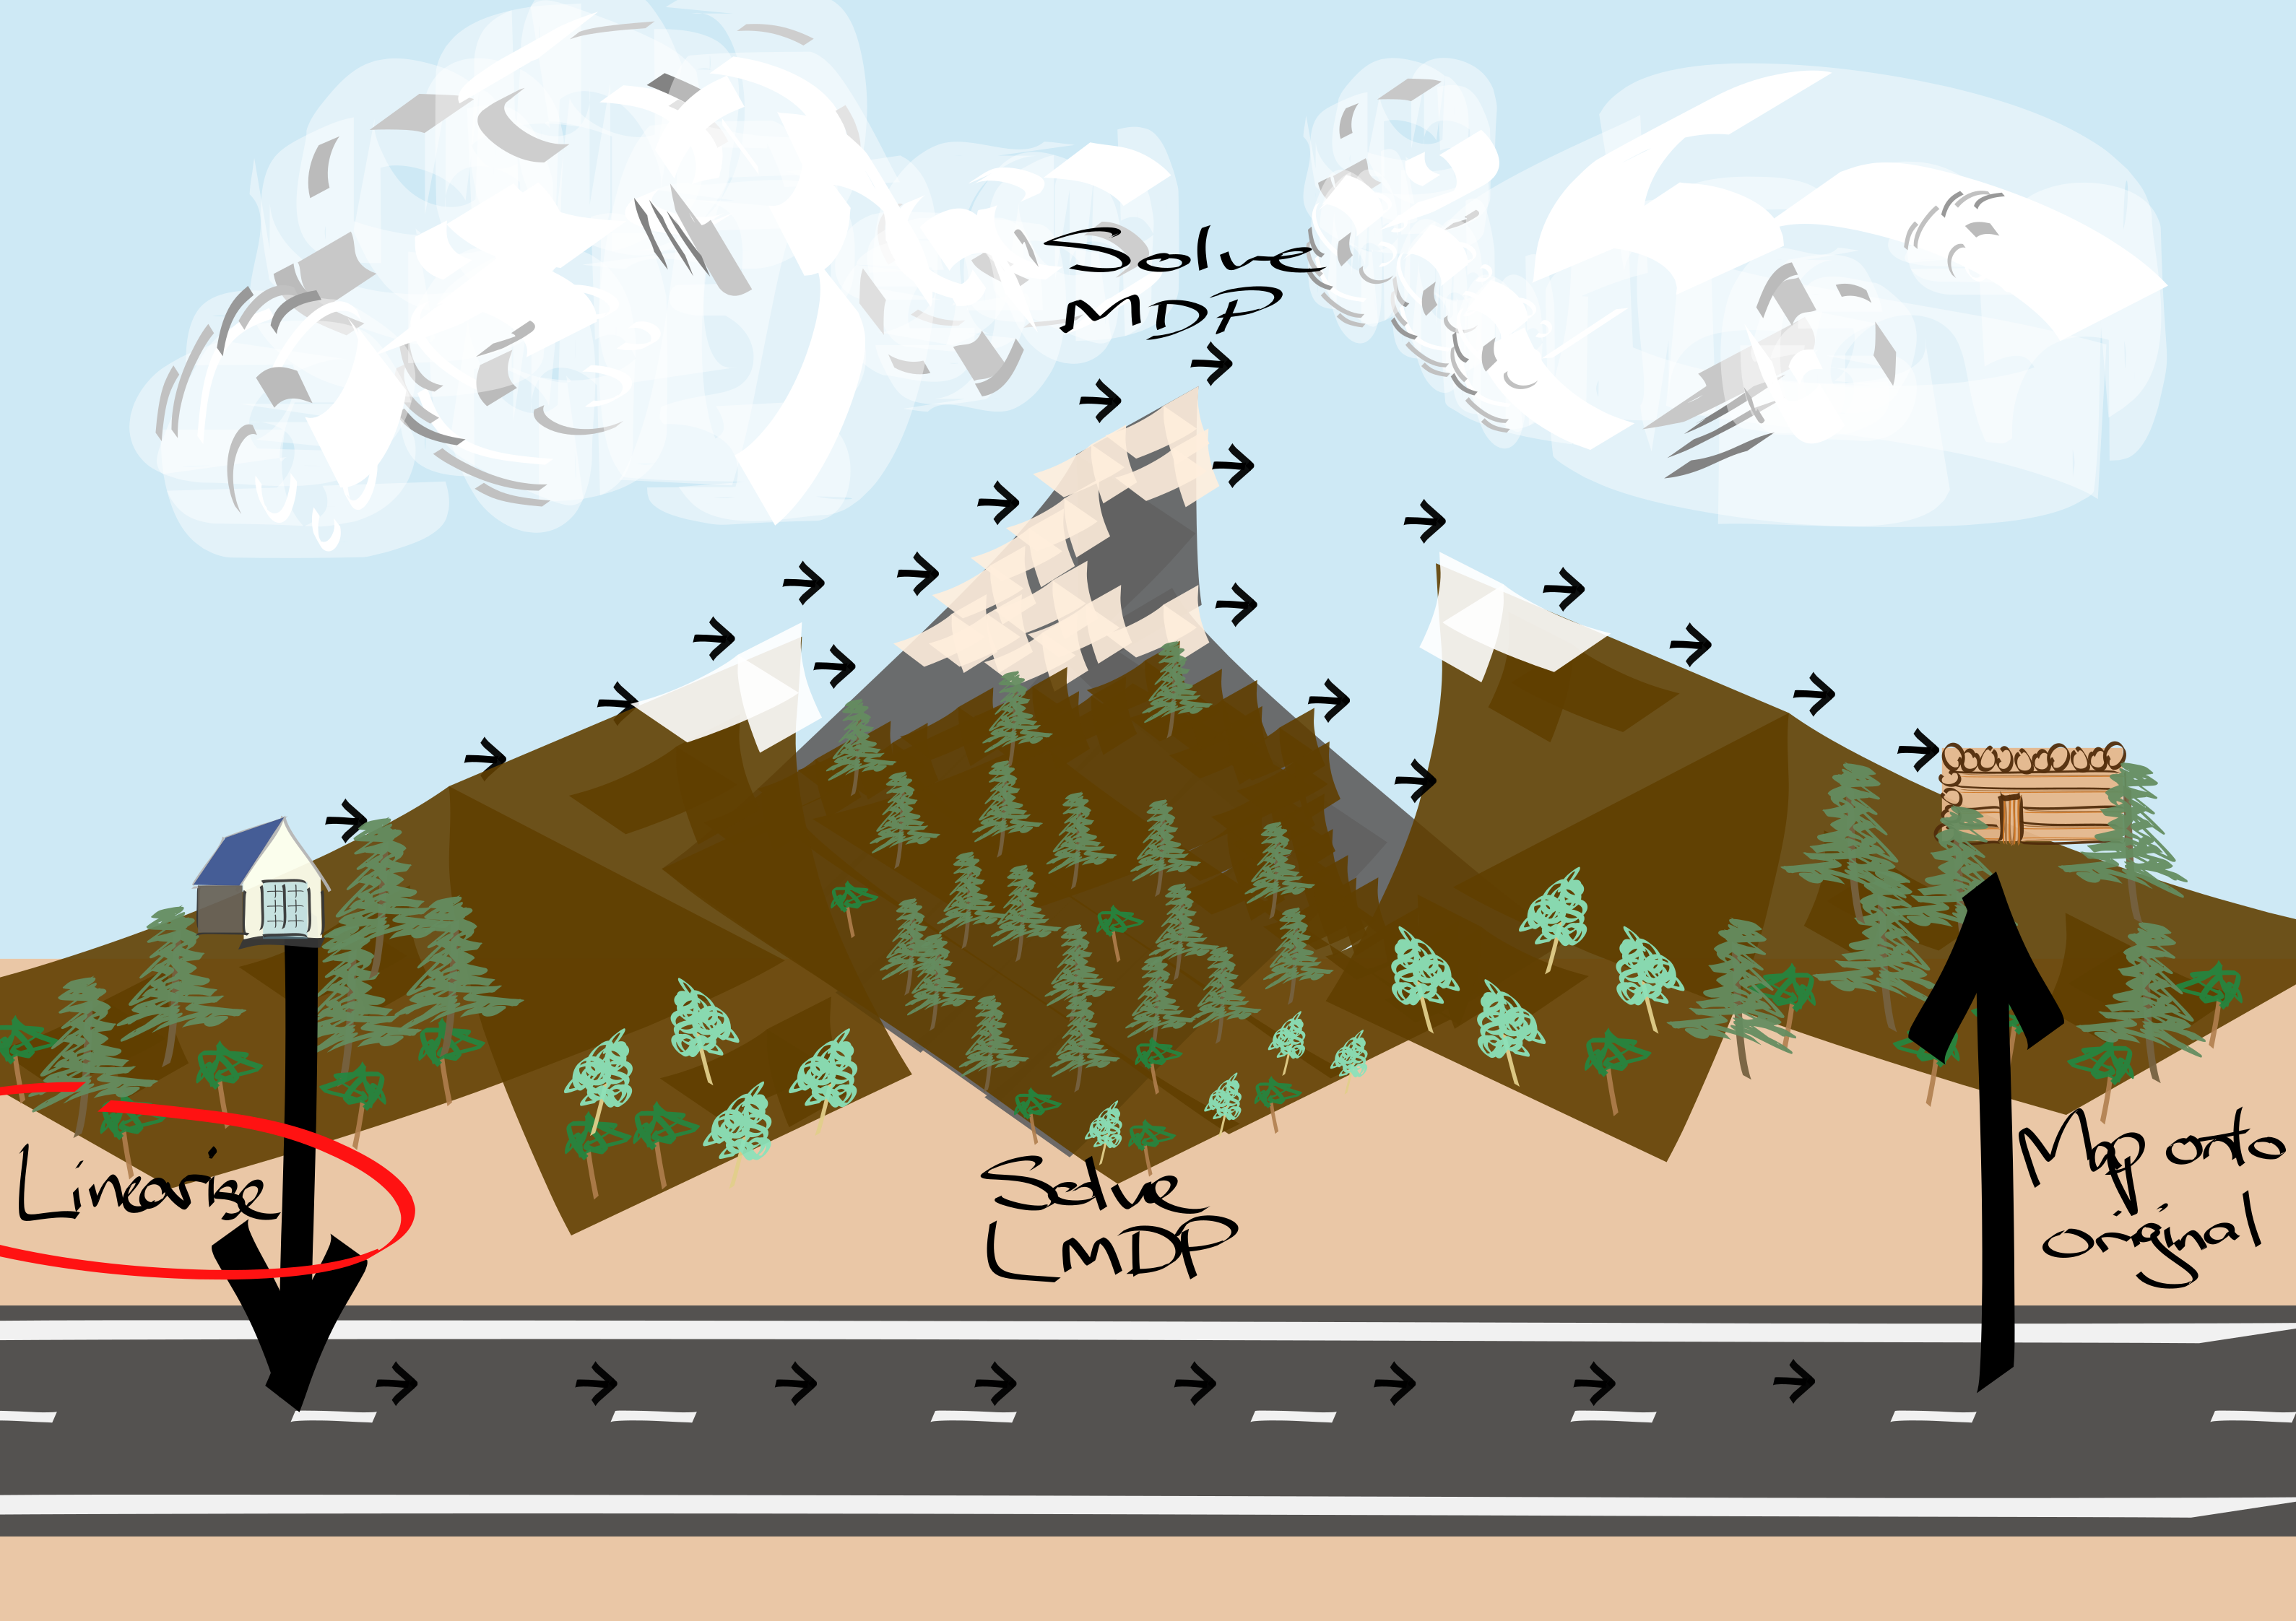
\includegraphics[width=0.6\textwidth,height=0.3\textheight]{../../pictures/drawings/abstract-representations-linear.png}
\caption{Solving a MDP}
\end{figure}

\begin{displayquote}
\textsl{So, LMDPs can be easily solved. But how does solving a LMDP help us solve a MDP?}
\end{displayquote}

We need a way to transform a MDP into a LMDP, while preserving the
`structure' of the original MDP. But what do we mean by a MDP's structure?
According \cite{Todorov2009}, the LMDP should be able to represent the same \ref{state-reward-rep} as the original MDP,
and give the the same \ref{unconstrained-dynamics-reward} was the original MDP.

\begin{align*}
\forall s, s' \in S, \forall a \in A, \exists u_a& \;\;\text{such that;} \\
\tau(s' | s, a) &= u_a(s'|s)p(s'|s) \tag{transition dynamics} \label{state-reward-rep} \\
r(s, a) &= q(s) - \text{KL}(\tau(\cdot | s, a) \parallel u_a(\cdot| s) ) \label{unconstrained-dynamics-reward} \tag{rewards}
\end{align*}

% "We do not yet have theoretical error bounds but have found the approximation to be very accurate in practice" \cite{Todorov}

So, given a reward function, $r$, and a transition function, $P$,
(from an MDP), we can use the \ref{state-reward-rep} and \ref{unconstrained-dynamics-reward}
to solve for the unconditioned dynamics $p$ and a state reward $q$.
This transformation, from $P, r \to p, q$ requires $|S| \times |A|$ computations, as for each state in the
MDP we need to satisfy constraints for each action. For a derivation and explanation see appendix \ref{mdp-Linearisation}.

However, an important condition is missing!
We should preserve the value of optimal actions (as discussed in \ref{efficient-control}).
Alternatively, we might settle for preserving the optimal policy.

\begin{align*}
\forall s, s' \in S, \forall a \in A, \forall \pi \in \Pi \\
z_{u_{\pi}}(s) = e^{V_{\pi}(s)} \label{value-preserved}\tag{value} \\
\tau(s'|s, a) \cdot \pi^{* }(a|s) = u^{* }(s'|s) \label{opt-policy-preserved}\tag{optimal policy}
\end{align*}

Where $z_{u_{\pi}}$ is the value (as evaluated by the LMDP) of the control $u_{\pi}(s'|s) = \tau(s'|s, a) \cdot \pi(a|s)$, and $V_{\pi}$ is the expected return of policy $\pi$ as evaluated by the original MDP.

It seems that Todorov hopes that the constraints \ref{state-reward-rep}, \ref{unconstrained-dynamics-reward},
will be sufficient to give \ref{value-preserved}, \ref{opt-policy-preserved}. But he does not prove it.
This is a problem that we will return to in \ref{paths}.

\subsection{Lifting the optimal LMDP policy}\label{lift-mdp}

\begin{figure}[h!]
\centering
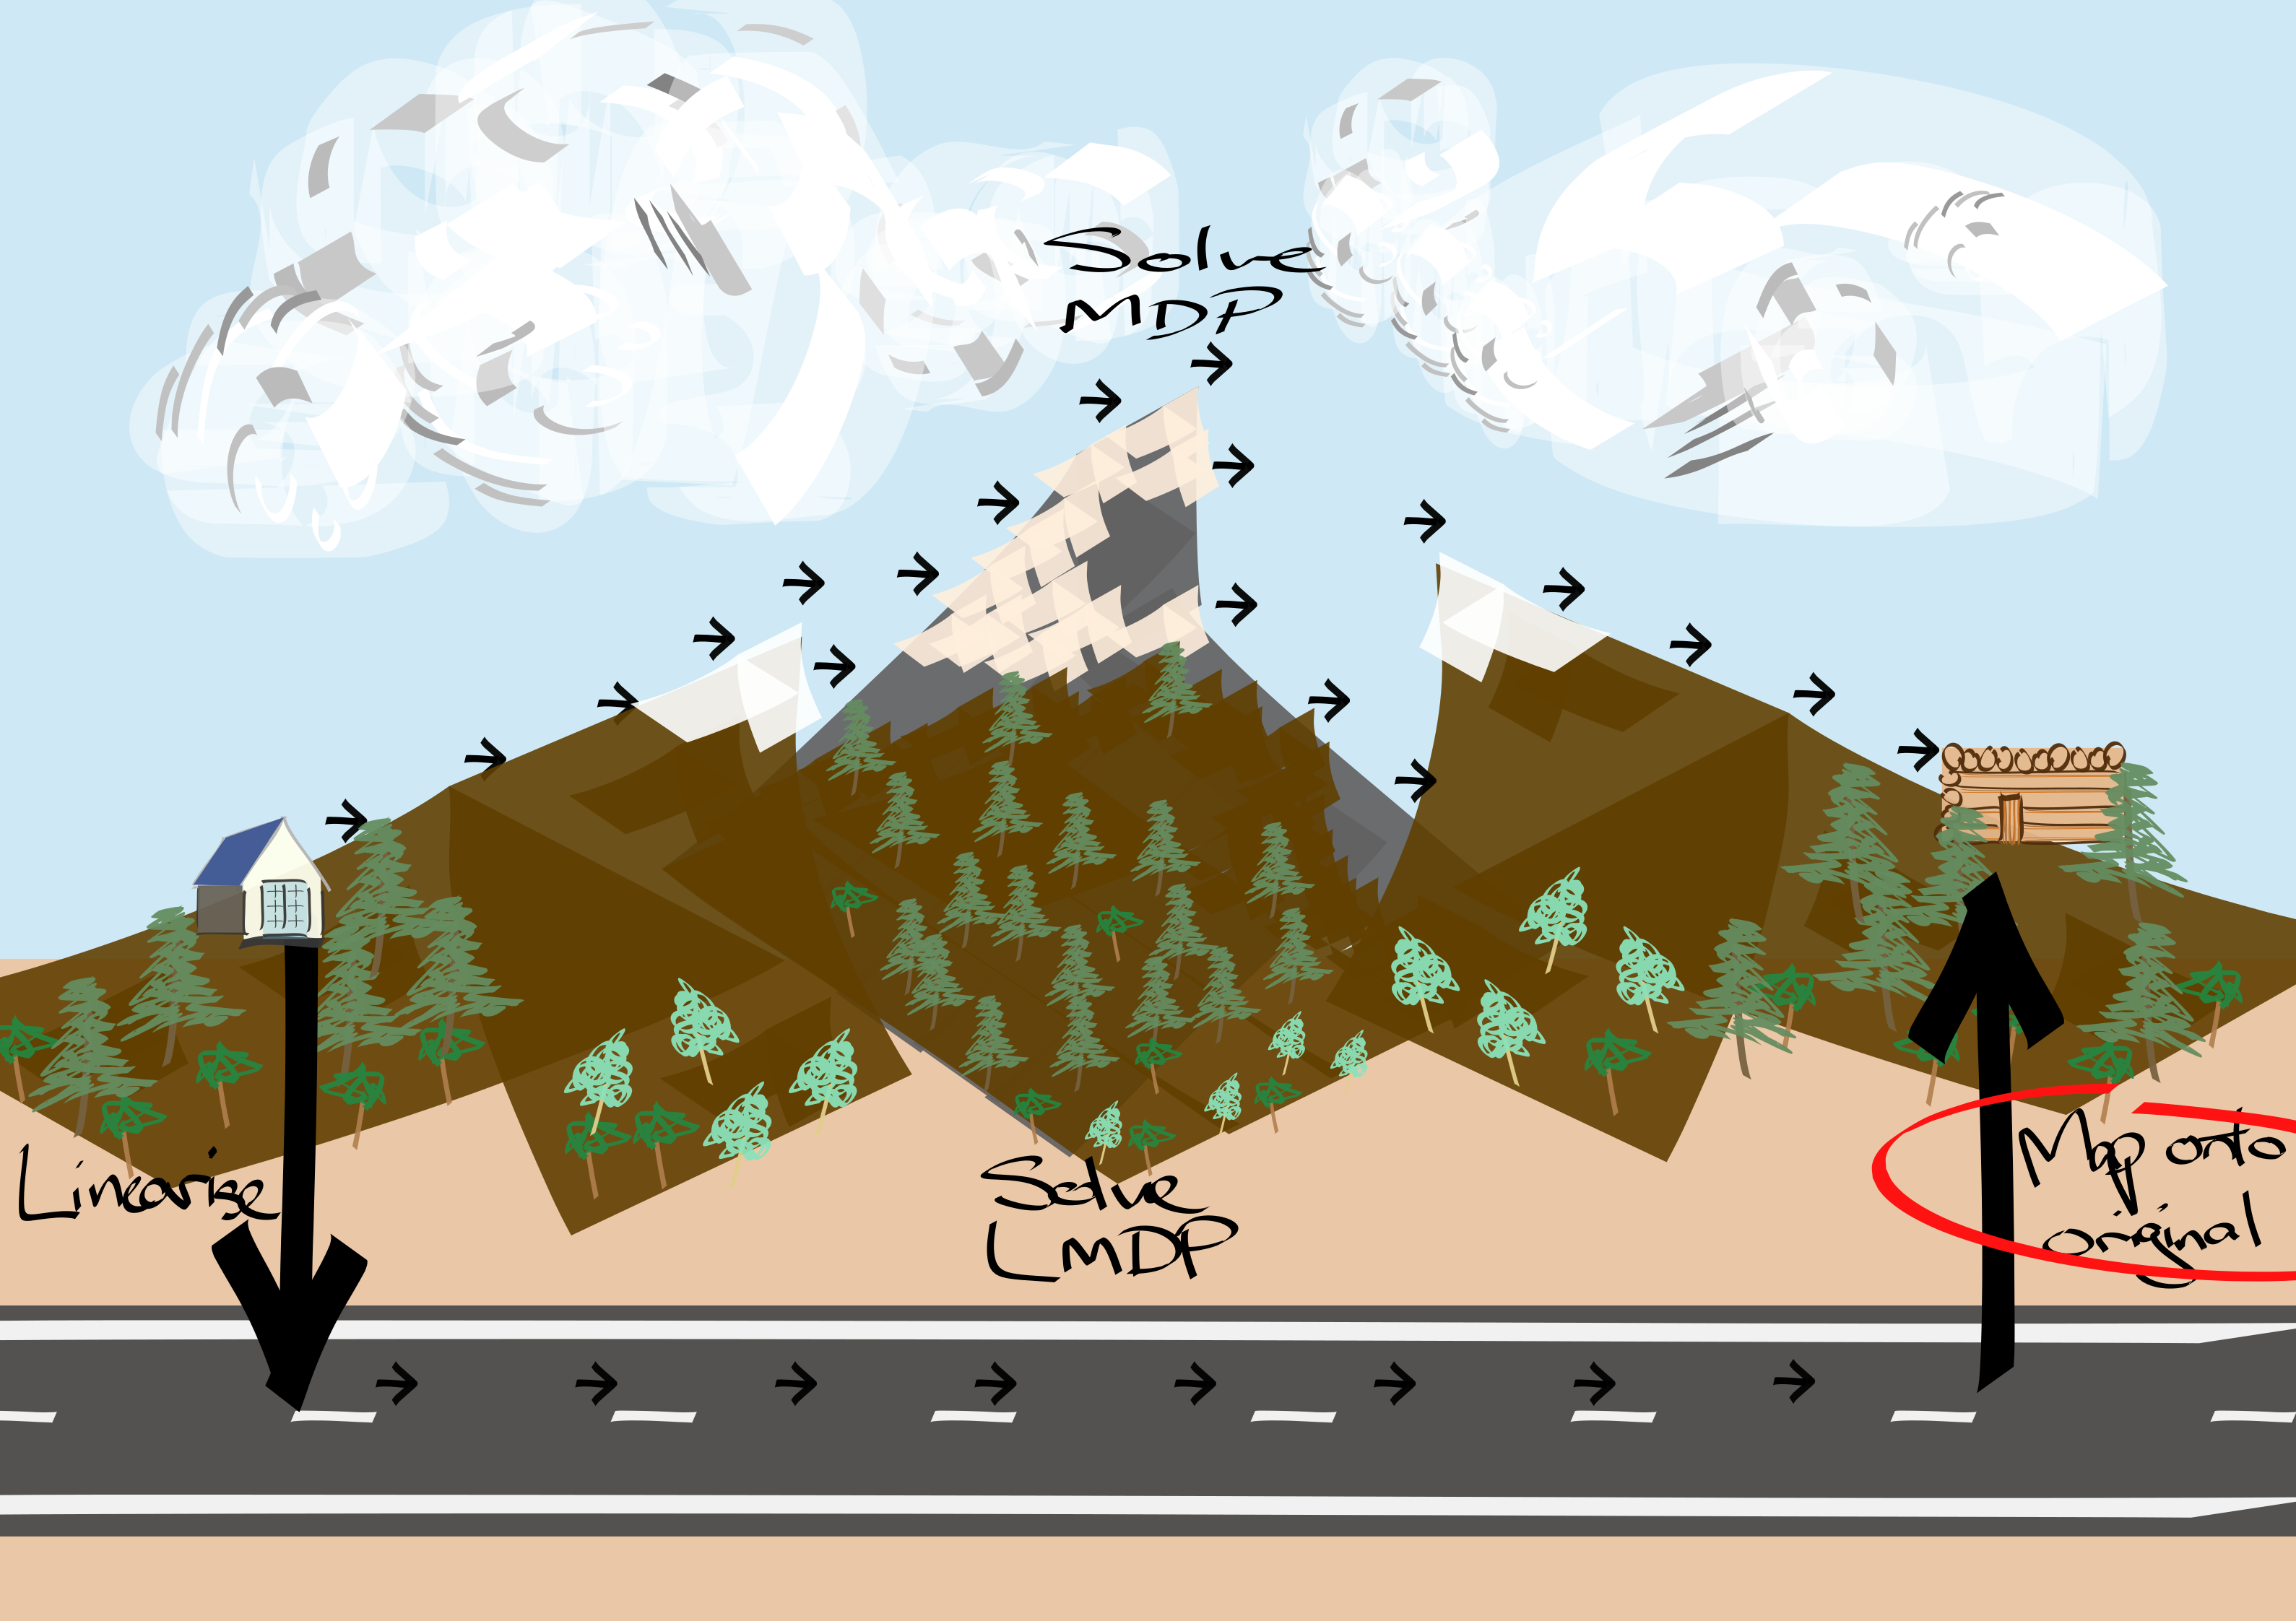
\includegraphics[width=0.6\textwidth,height=0.3\textheight]{../../pictures/drawings/abstract-representations-project.png}
\caption{Lifting the LMDP's solution to the MDP}
\end{figure}

\begin{displayquote}
\textsl{How can we use the optimal control, $u^{* }$, to construct a policy that is optimal in the original MDP, $\pi_{u^* }$?}
\end{displayquote}

The LMDP has disentangled the search for the optimal controls (solve the LMDP) (go to this or
that state) from the search for the optimal policy (how to actually
realise that control).

This decomposition is reminiscent of goal conditioned approaches to hierarchical RL.
Where a higher level agent gives goals (go to this or that state) to a lower level
agent, who must figure out how to achieve that goal \cite{Vezhnevets2017}.

This decomposition within the LMDP can be seen as the optimal control decoding
step (currently being considered). We know which
states we want to be in, the $z^{* } / u^{* }$, from solving the LMDP, but,
we do not know how to implement those controls with the actions we have available in the original MDP.
We can formulate this problem as;

\begin{align*}
\tau_{\pi}(\cdot | s) = \sum_a \tau(\cdot | s, a) \pi(a | s) \\
\pi = \mathop{\text{argmin}}_{\pi} \text{KL}\Big(u(\cdot | s))\parallel \tau_{\pi}(\cdot | s)\Big)
\end{align*}

We would hope that the knowledge of $u^{* }$ would make it easy to find the optimal actions.
But, this optimisation problem has very little structure for us to exploit.
In the worst case it has complexity $\mathcal O(|S|^2|A|)$ (which is the same as solving a MDP).

\begin{center}\rule{0.5\linewidth}{\linethickness}\end{center}

We have now built a way to solve a MDP with a LMDP.
We have a method to transform a MDP to a LMDP \ref{construct-lmdp-from-mdp}.
We can solve the LMDP \ref{solve-lmdp}.
Finally, we can lift the solution to the original MDP \ref{lift-mdp}.
Let's try it out.

\subsubsection{Optimality of solutions via LMDPs}\label{paths}

\begin{quote}
\textsl{Do these two paths lead to the same place?}
\end{quote}

One of the main questions we have not addressed yet is; if we solve the
MDP directly, or we linearise then solve then lift, do we end up in the same
place? This is a question about the sub-optimality of our abstraction \ref{near-optimal-abstraction}. Can
our abstraction approximately represent (and find) the same solutions that the
original can? We can formalise this question as the difference between the optimal values or optimal policies.

\begin{align*}
\epsilon &= \parallel Q_{\pi^{* }} - Q_{\pi_{u^{* }}} \parallel_{\infty}
\end{align*}

We answer this question using experiments, described in figures \ref{fig:ltd} and \ref{fig:opt-control}.

\begin{figure}[h!]
\centering
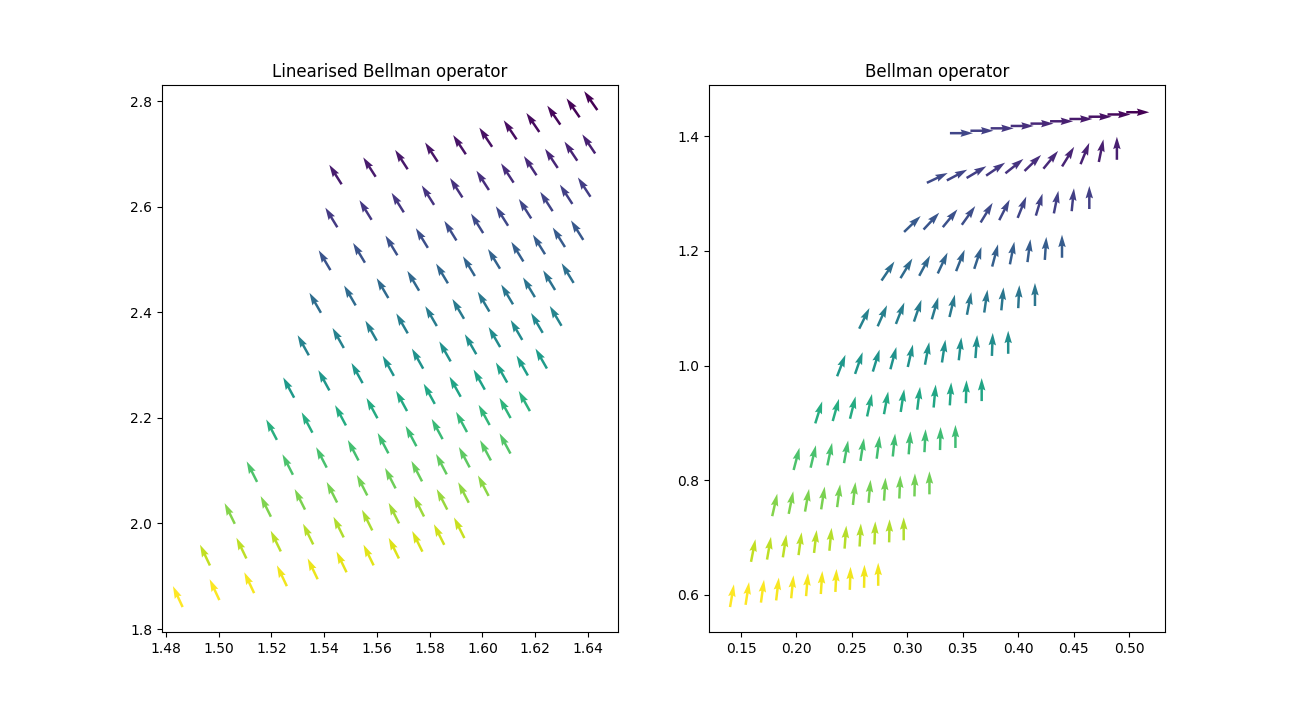
\includegraphics[width=0.75\textwidth,height=0.5\textheight]{../../pictures/figures/LBO_BO.png}
\caption{For the same MDP, shown is a comparison of the linear temporal difference operator (left), versus the true, Bellman, temporal difference operator (right). As expected, the temporal difference operator points towards the optimal value. But, the linear temporal difference operator points elsewhere.}
\label{fig:ltd}
\end{figure}

\begin{figure}[h!]
\centering
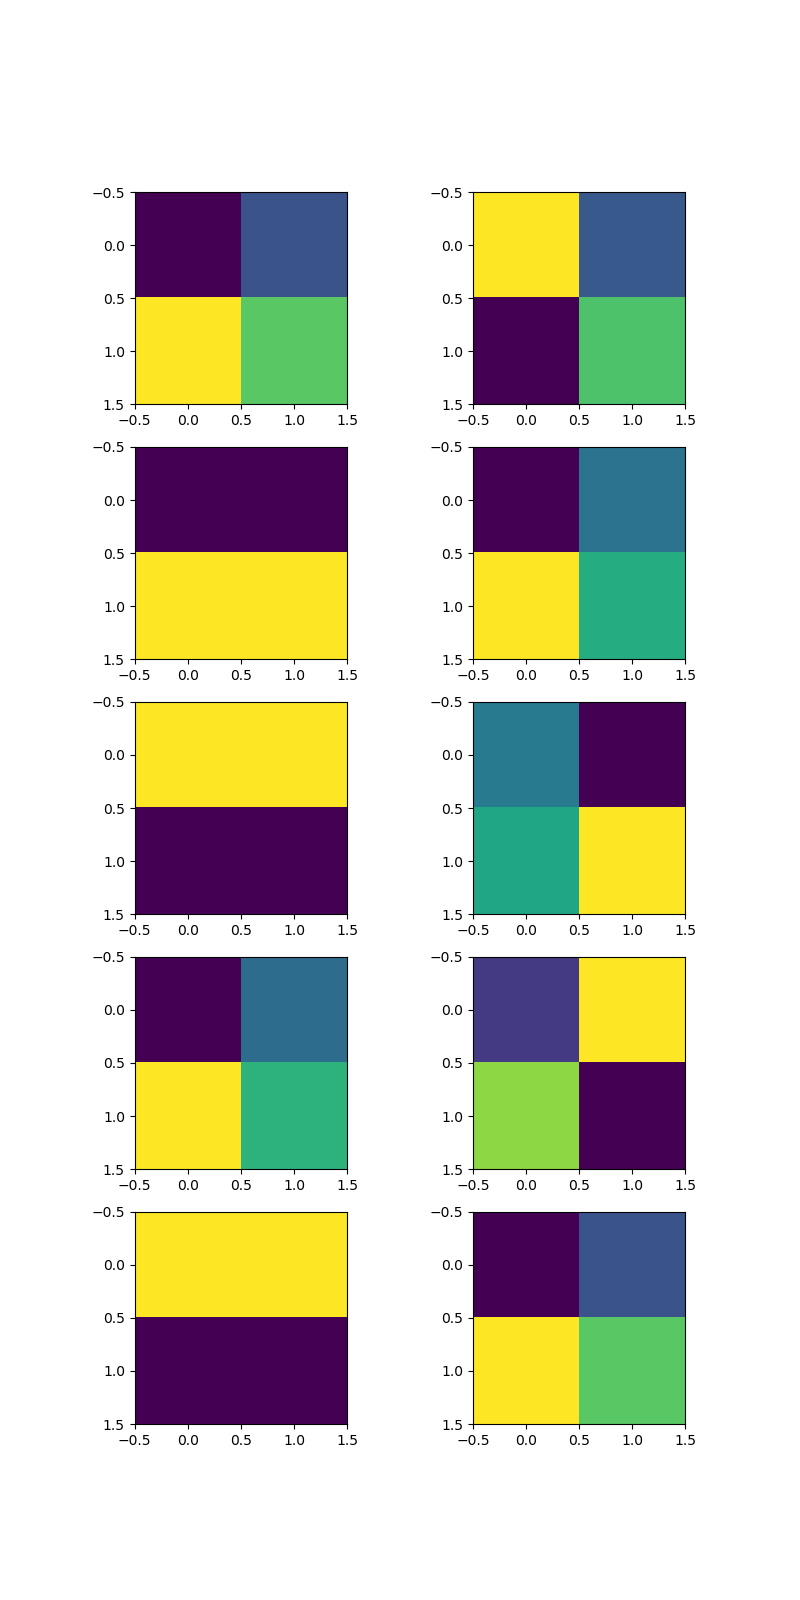
\includegraphics[width=0.5\textwidth,height=0.75\textheight]{../../pictures/figures/lmdp_mdp_optimal_dynamics.png}
\caption{A comparison between the optimal control $u^{* }(s'|s)$ (shown in the left column) and the dynamics of the optimal policy (MDP) $\sum_a \tau(s'|s, a)\pi^{* }(a|s)$ (shown in the right column). Because the optimal control, and dynamics of the optimal policy can be written as $2\times 2$ matrices, we can plot them. Yellow indicates high probability, purple indicates low probability. But the main thing to observe is that the optimal control is often not the same as the dynamics of the optimal policy.}
\label{fig:opt-control}
\end{figure}

We also investigate the sensitivity of the LMDP's optimal control given different MDPs.
The optimal control is very sensitive to the sign and magnitude of the rewards, as can be seen in \ref{fig:chain-zero} and \ref{fig:chain-pos}.

\begin{figure}[h!]
\centering
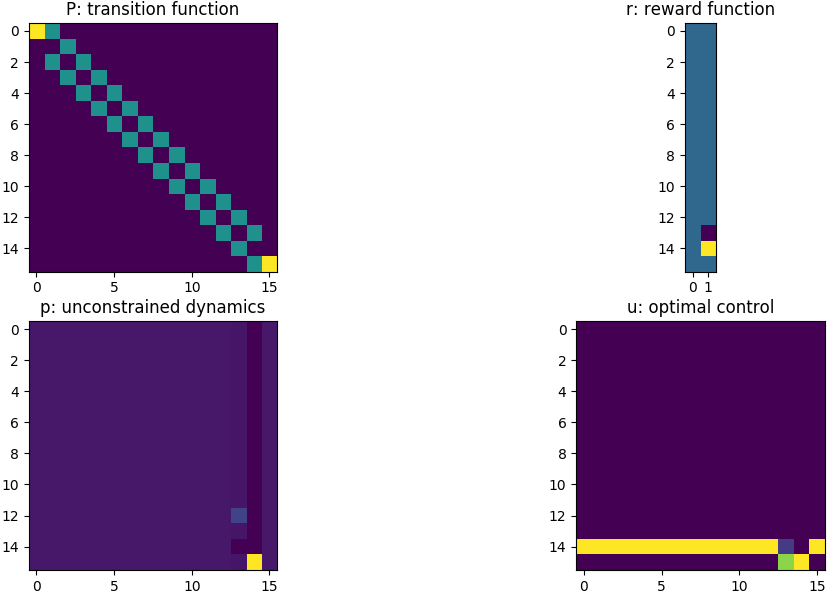
\includegraphics[width=0.65\textwidth,height=0.325\textheight]{../../pictures/figures/chain-test-zero-rewards.png}
\caption{A chain problem \cite{Sutton2018a} with zero reward on all states except the last two. A small negative reward, then a large positive one.
The optimal control to this problem is not realisable: in every state, jump to the state with positive reward.}
\label{fig:chain-zero}
\end{figure}

\begin{figure}[h!]
\centering
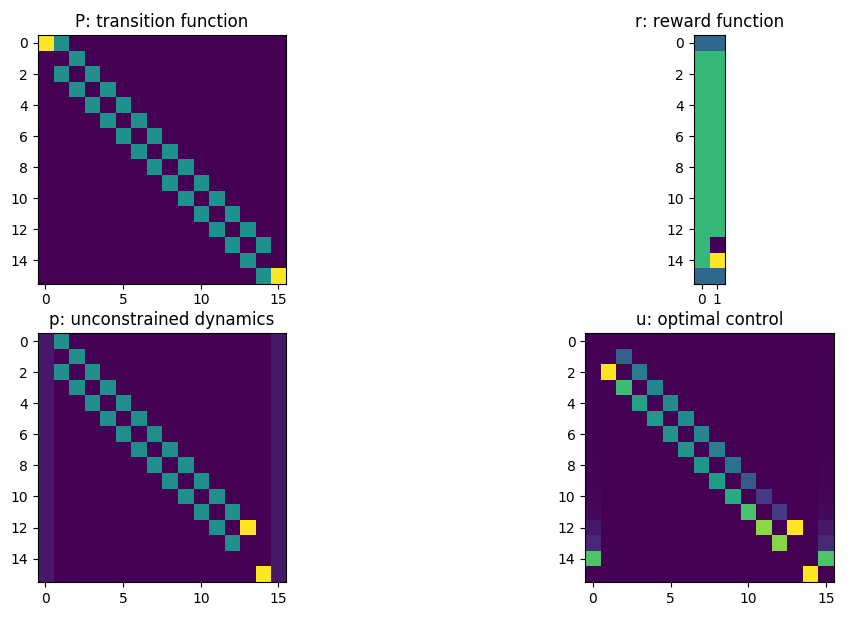
\includegraphics[width=0.65\textwidth,height=0.325\textheight]{../../pictures/figures/chain-test-pos-rewards.png}
\caption{The same chain problem as above, but with an positive reward added to all states.
We can see that the structure of the transition function has now made it into the optimal control!
The LMDP's control can be decoded into a realisable policy.}
\label{fig:chain-pos}
\end{figure}

\newpage
\subsection{Discussion}\label{lmdp-validation}

Unfortunately, Todorov \cite{Todorov2006,Todorov2009} never actually produced
any experiments that use the linear bellman equation to solve a MDP.
His experiments were with $Z$-learning, the linearised counterpart to $Q$-learning.

\begin{align*}
\tilde z(s) = e^{q(s)}z(s{'})^{\gamma} \tag{linearised bellman eqn}\\
z_{t+1}(s_i) = (1- \eta)z_{t}(s_i) + \eta\tilde z(s_i) \tag{$Z$ iteration}\\
\end{align*}

He makes this work by hand picking $q$ so that the optimisation will converge to the optimal value.
Then he evaluates the accuracy of the value estimates.
They do not give a general way of constructing $q$ from a MDP that actually works (in the sense of yielding the same optima).
Nor do they give an efficient way to map an optimal control to an optimal policy.

% \begin{figure}
% \centering
% 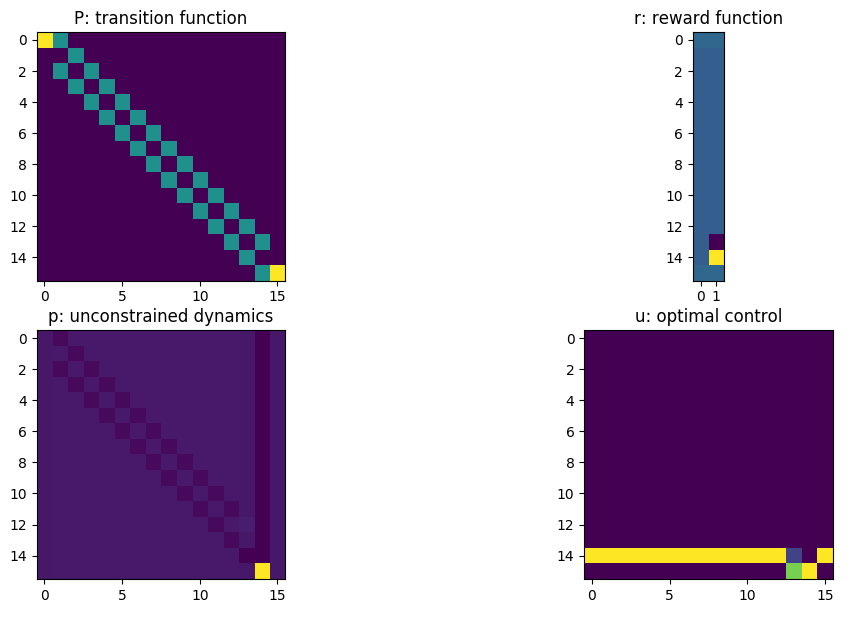
\includegraphics[width=1\textwidth,height=0.35\textheight]{../../pictures/figures/chain-test-neg-rewards.png}
% \caption{A chain problem with negative rewards applied to all states.
% Again, the structure of the transition function is missing.}
% \end{figure}

Because there are no benchmarks that we can validate our implementation on,
there is some doubt about whether I implemented the LMDP correctly. While the
LDMP solution strategy does occasionally pick the correct optimal policy, more often than not,
its outputs are seriously wrong.

\subsubsection{Linearity in MDPs}

Todorov's formulation of LMDPs does not seem to allow a MDP to be to reliably embed a LMDP.
Despite this, it might still be possible to construct a linear MDP given different assumptions.

Let's reconsider Jin et al.'s approach \cite{Wang}: construct a MDP where the value is a
linear function of a state-action representation and of a policy embedding.
It is important to note that, not every (policy) embedding can be realised as a policy, so to constrain the search dynamics properly
we must use the Bellman equation.

And this captures the essence of the problem. We need the Bellman equation for efficient search, but it is not linear in the policy.
So, we can linearise a MDP, but we will lose the ability to use the Bellman equation to guide the search for the optimal policy.

% Refs \cite{Todorov2006,Todorov2009,Zhong,Zhonga,Dvijotham,Wozabal}
% Linearise around the optimal policy. But how does that tell us how to act when not at the optimal policy?

\newpage
\section{Symmetric abstractions}\label{symmstric-abstractions}


% Reasonably well understood how symmetric abstractions can improve computational complexity.
% But, want to understand how they effect sample complexity.

% symmetry is cool
Symmetry is a concept from pure mathematics, which has found major success in physics, ...
(why has it found such success in physics? beauty, compression, ... Occam's razor)
But what do we mean by symmetry?

% example


% occam's razor
Occam's razor is a core idea behind much of statistics, ML and science. Simple
hypotheses should be preferred as the are more likely to be right. This intuition
can be viewed a little more formally through a Bayesian perspective.

% symmetry and occams razor
How does symmetry relate to simplicity?

% how can symmetry help? more concretely
But, why do we care about symmetry?
\begin{displayquote}
We want the ability to identify symmetries in state-actions-rewards (/values) and use that knowledge to share rewards (/values) between 'similar' state-actions.
\end{displayquote}
It gives us a way to find 'simple' hypotheses that fit the data.
Imagine we knew that a learning problem was symmetry in some sense, for example ...
How might we exploit this knowledge to learner more efficiently?
Reduce variance, generalise in more 'intelligent' ways.

% but. discovery
But.

% relation to abstraction
???

% related work on complexity / occam's razor
This ability is currently lacking in the ML tool kit. There has been much work done
to

%  why do we care?
For sample efficiency!! Inductive bias. Generalise in the right way without making observations.

\subsubsection{Definition}

?!?!
The most useful starting point. Finite groups.

A group is a set, $G$, together with an operation $\circ$ (called the group law
of $G$) that combines any two elements $a$ and $b$ to form another element.
To qualify as a group, the set and operation, $(G, \circ)$, must satisfy four requirements known as the group axioms:

\begin{itemize}
	\tightlist
	\item \textbf{Closure:} For all $a, b \in G$, the result of the operation $a \circ b$ is also in $G$.
	\item \textbf{Associativity:} For all $a,b,c \in G$, $(a\circ b) \circ c = a\circ (b\circ c)$.
	\item \textbf{Identity element:} There exists and element $e\in G$ such that, for every element $a\in G$, the equation $e\circ a = a\circ e = a$ holds.
	\item \textbf{Inverse element:} For each $a \in G$, there exists an element $b \in G$, commonly denoted $a^{−1}$, such that $a \circ b = b \circ a = e$.
\end{itemize}

\subsection{Symmetries for RL}\label{mdp-homomorphism}

Which types of symmetry can exist in RL problems?
% How hard is it to find these symmetries?
% Are some harder than others?

\begin{figure}[h!]
	\centering
	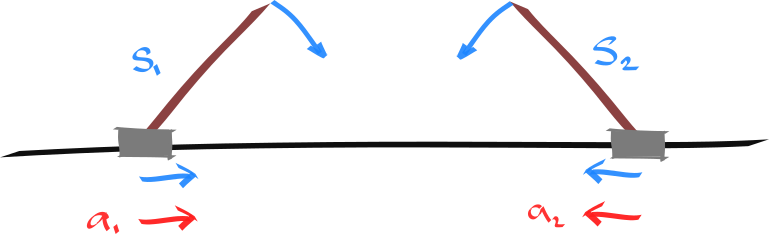
\includegraphics[width=1\textwidth,height=0.25\textheight]{../../pictures/drawings/cart-pole-mirror.png}
	\caption{Two mirror symmetric states of a cart pole.}
\end{figure}

% Need to show this is actually a symmetry, isomorphic to $S_2$?!?

These two objects are symmetric about a mirror plane (Need to draw).
Symmetric because there exists $f$ such that ...

% Want symmetry for efficient exploration / sample efficiency. !!!!
% Rather than picking actions; randomly, to minimise uncertainty, to ...?
% We want to pick actions to help us identify symmetries in the MDP.
% How does this help us increase the sample efficiency?
%
% If we are using something like neural counts. How does it generalise it density estimates!?
% Want symmetries!!!

\vspace{5mm}

As pointed out in \ref{abstraction}, the notion of an abstraction is captured by a homomorphism.
So, what would it look like if we had a MDP homomorphism?

What does it preserve?!?!

\cite{Ravindran2002}

$\mathcal H: \mathcal M\to \mathcal M$.

\begin{align}
P(f(s')|f(s), g_s(a)) = \sum_{s''\in [s']_f} P(s''| a, s) \\
r(f(s), g_s(a)) = r(s, a)
\end{align}


To be done.

\begin{itemize}
\tightlist
  \item temporal symmetries
  \item approximate symmetries (algorithm and complexity)
  \item inference of symmetries under uncertainty (algorithm and complexity)
  \item complexity measure / inductive bias
\end{itemize}

\subsection{Exploitation}

\begin{displayquote}
\textit{Once have discovered a symmetry, how might we exploit that knowledge?}
\end{displayquote}

\subsubsection{Exploiting symmetry for efficient control}

% Simple and well demonstrated.

Model minimisation. (are there any alternatives?)

...\cite{NARAYANAMURTHY}

\subsubsection{Exploiting symmetry for efficient inference}

\cite{Chen2019}
\ref{symmetry-inference}

\subsubsection{Exploiting symmetry for efficient exploration}

\cite{Holtzen2019}

Want to demonstrate this.
{\color{red}TODO max ent + abstraction experiments}

\subsection{Discovery}

% This is about generalising using an inductive bias towards symmetry.

Symmetry is a stricter notion of similarity. How can it be discovered?

Relationship to disentanglement. \cite{Higgins2018} which makes a lot of sense because ...

Connection to causal hierarchy. Cite Pearl. Association, intervention, counterfactuals.
Also recently noted by \cite{Caselles-Dupre2019}, ... where they assume that
the group actions are the actions of the RL environment.
This doesn't really make sense. Also, will miss many symmetries like ???

A couple parts. Discovery of symmetries, exploration of the knowledge of symmetries.

Unsupervised discovery. Not much success yet. Only when using some kind of supervised signal.

\cite{Ho2019a, Lim2019, Cubuk2018, Cubuk2019}
Discover which symmetries apply to a given domain, and at what magnitude.
The optimisation problem becomes one of picking the probability of each op and its magnitude.
There is a small set of ops (aka symmetries) that are given:
\textit{Identity, AutoContrast, Equalize, Rotate, Solarize, Color, Posterize, Contrast,
	Brightness, Sharpness, ShearX, ShearY, TranslateX, TranslateY.}
Uses validation error as a reward for learning.


\subsubsection{Inferring symmetries from experience}

% How easy is it to solve this symmetry inference problem?

% HOW?!

What does this buy us? If have sufficient data to tell us that $x$ and $y$ are
similar, say that they are mirror images of each other.
As an unsupervised pre-training step. Then apply and share labels and learn more quickly?
What else can $x$ tell us about $y$?

\cite{Yang2019}

Or end to end? As we get more certain that x and y are similar, we more strongly
encourage their symmetry through one of the methods outlined above.
Is it possible (/easier) to learn that x and y are similar (in terms of their labels) before (accurately) learning their labels.



Want to have an inductive bias towards simpler symmetries. But, how can we do this without needing to represent all possible symmetries?
A solution rejection sampling??


%
% - What about symmetries that are products of subgroups? $S = Z_2 \times Z_3$?
% Are they easier to infer?
% - Within the same $n$. Is there a notion of more or less complex group structures??
% - Need to show that NNs dont have the right symmetric inductive bias. They dont generalise. !!!

% Examples

% - Knowing that; range $= [0,360)$, and $0, 45, 90, 135, 180$, all are similar. I guess that we are in cyclic group $8$ and therefore $225, 270, 315$ are also similar. Key is that I know that $0, 45, 90, 135, 180$ are related by $0+0, 0+45, 0+45+45, 0+45+45+45, 0+45+45+45+45$.
% - Cart pole. $V^{\pi(s, a)}(s') = V^{\pi(-s, -a)}(-s') \forall s'$.


\subsubsection{Invariants}

Symmetries can be uniquely characterised by their invariants \cite{PeterOlver1999}.
What are the interesting invariants of MDPs? And how do they ???
But, what does this symmetry imply about other quantities of interest for RL?

Invariance, $f(g(x)) = f(x)$, equivariance, $f(g(x)) = g(f(x))$.

In general we want to know;

\begin{itemize}
	\tightlist
	\item We have $n$ different 'symmetries'. But are they really different?
	\item Which symmetries share some invariants?
	\item Which invariants uniquely characterise this symmetry?
\end{itemize}

With this knowledge, we could identify symmetries via their invariants!?!
We can observe invariant properties. (not clear to me how you observe a symmetry!?)

We briefly explore this in \ref{game-invariants}.


\subsubsection{Inductive bias towards seeing symmetry}

% WANT GENERALISATION!

The problem is the cost of inferring symmetry

Guess that things are symmetrc, despite observing they are not.

\begin{align}
P(\tau, r| \theta)
\end{align}

Clip to nearest symmetric abstraction.

Have a prior belief that MDPs are sampled from $M \sim ???$.


\subsection{Thompson sampling} \label{thompson-sampling}

{\color{red}TODO need to introduce this framework}

SARSA plus thompson sampling. Does this really work? Want to test.

\begin{algorithm}
	\caption{Thompson sampling}
	\begin{algorithmic}[1]

		\Procedure{TS}{$\gamma$}
		\State $\pi_t \sim \mathcal U(\Pi)$
		\While{not converged}
		\State $\tilde P, \tilde r \sim P_{\theta}(\cdot)$
		\State $Q_{t+1} =  r + \gamma P Q_t$ \Comment{Bellman operator}
		\State $\theta = \nabla_{\theta} P_{\theta}(P, r)$ \Comment{Max likelihood}

		\EndWhile
		\State \algorithmicreturn{ $\pi$}
		\EndProcedure

	\end{algorithmic}
\end{algorithm}

The way we parameterise the distribution over possible models (/ MDPs), $\theta$, has implicit inductive biases about the true structure of the model.
A way to add explicit inductive biases is via importance (/ rejection) sampling.

We can encourage the model to be more symmetric!?
How much computation does this cost?

But. How can we construct the distribution? We want to be able to take samples
from it.

Ok. Great we have this inductive bias. But it doesnt help exploration in the way I want it to...
The parameters we have learned are close to being symmetric in some way. So the complexity measure alters the likelihoods and makes the symmetric version the most probable.
How does this help exploration? More likely to sample the true model / a symmetric one. Need to be able to exploit this symmetry.

This solves the efficient inference problem. Not efficient exploration... How can we get both?
Sample an abstraction then lift it to the original MDP?!


Thompson sampling from estimates of similarity / symmetry.
\begin{enumerate}
	\tightlist
	\item Keep estimate of similarity. $\chi(x_i, x_j)_{t+1} = \chi(x_i, x_j)_t + ?$
	\item Construct distribution over likely abstractions $P(x_i = x_j) \propto e^{\chi(x_i, x_j)_t}$. $\mathcal F = P(f|\chi_t)$
	\item Sample an abstraction. $f\sim \mathcal F$
	\item Reduce the MDP $M' = f(M)$
\end{enumerate}


For now just assume we have an accurate estimate of the model.
What does acting optimally wrt the reduced model mean for exploration and convergence??


% How to reason about the tradeoff between symmetry and fitting the data!?.

\section{Action abstractions}


\epigraph{
A green leaf, is too far, out of reach,
What you want, is in front, take the steps.

You move your first leg up You move your second leg left ... You move your eleventh leg up You move your twelfth leg right

Many legs burden the act,
Unless coordinated in abstract.

The abstract words in this new language,
Must be as few as we can manage.

"left", "right", "forward", "backward"

This time, the act is rather brief,
"forward", to reach the tasty leaf.
}{\textit{The writer and poet: Alex Telfar}}


Action abstraction is possibly the least explored type of abstraction.
There exists a lot of work seeking state abstraction (refs), and heirarchical (temporal) abstraction (refs)
but, this has only recently been some work ...

\subsection{Interfaces}

The intution is.
People can generalise / adapt between different action spaces.

\begin{itemize}
\tightlist
\item
  Might be teleported to a new environment? (new state space, same
  action space)
\item
  Might have to drive a new vehicle (same state space, new action space)
\end{itemize}


Utility?
- Adapt to broken limbs
- To new ?

% ref sergey levine meta adaptation limb paper!?

\begin{figure}
\centering
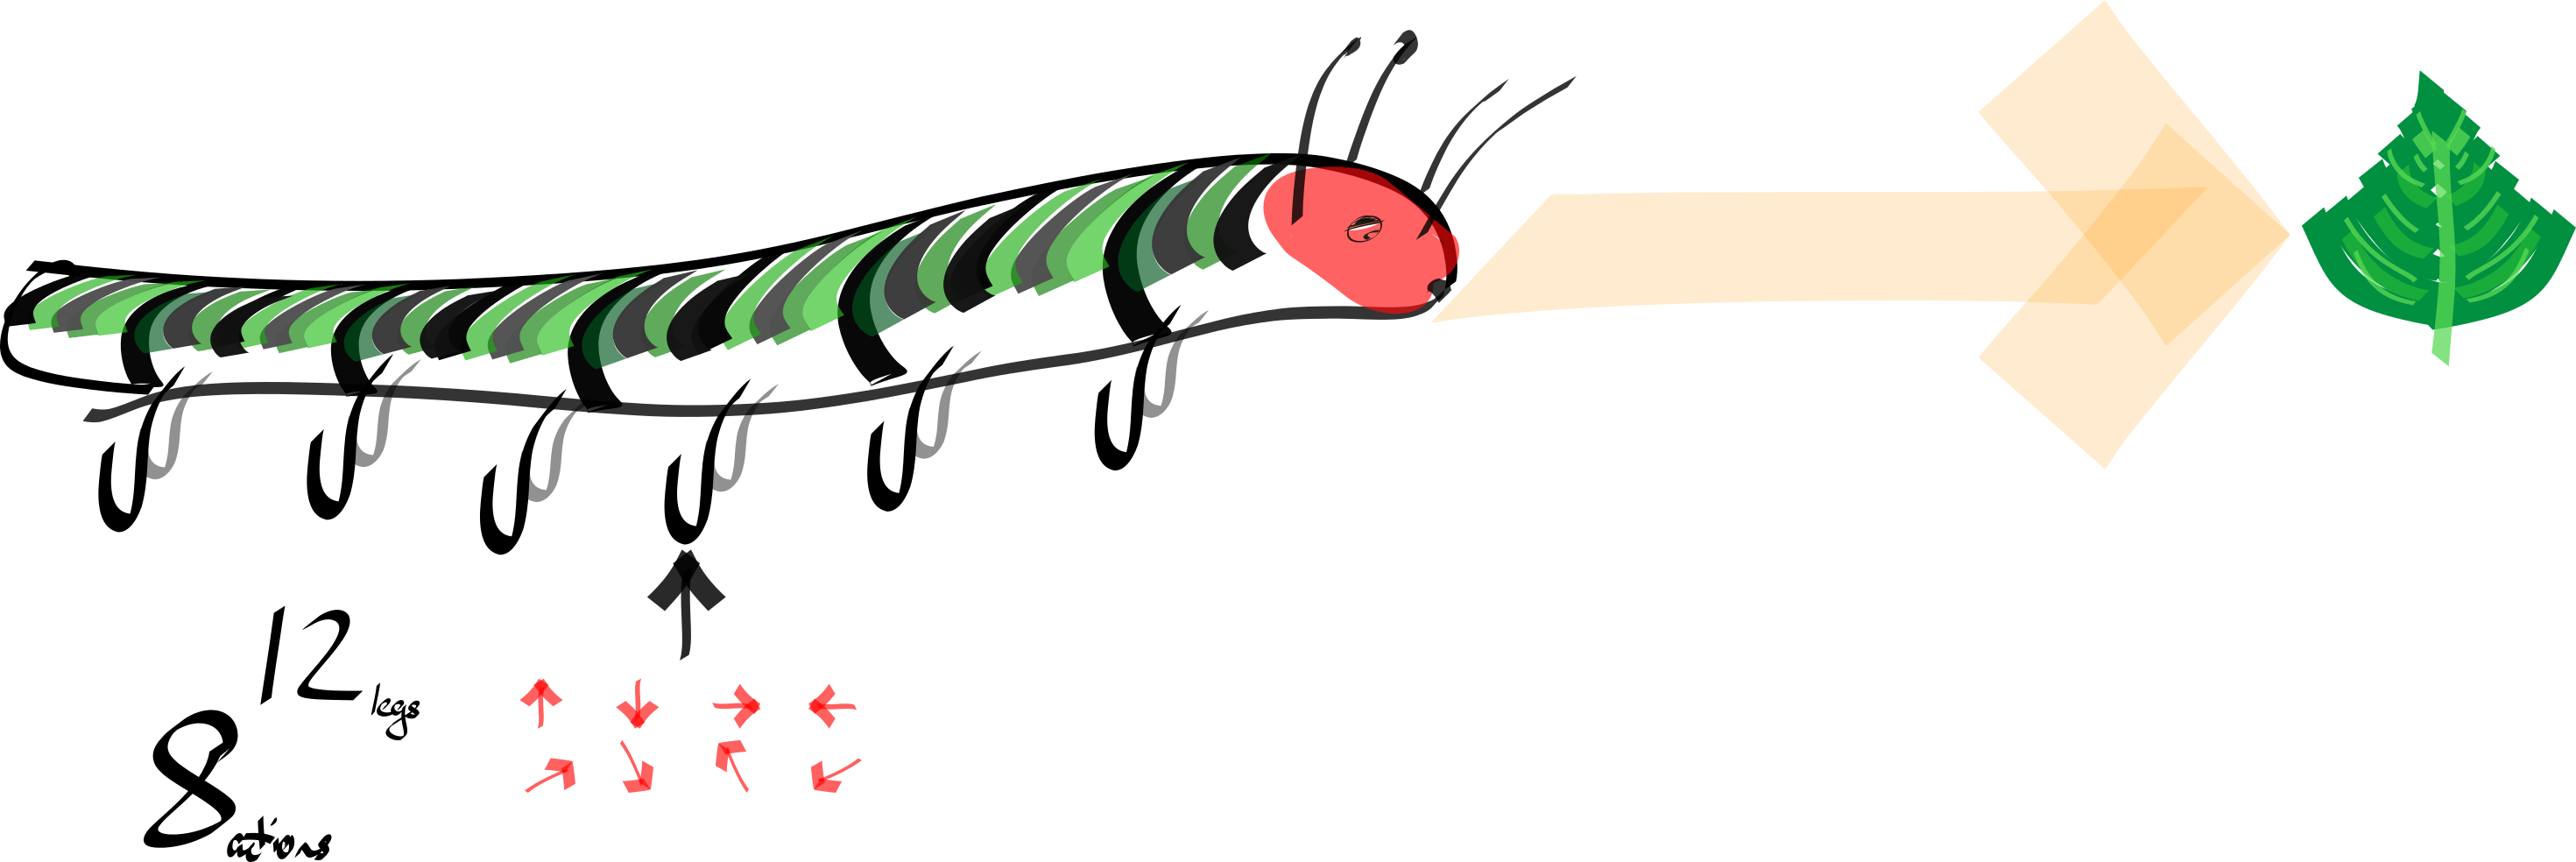
\includegraphics[width=\textwidth,height=0.25\textheight]{../../pictures/drawings/hungry-caterpillar.png}
\caption{Consider a hungry caterpillar. It wants to move towards the leaf. But this is a complicated task! Move your 3rd leg up, your 7th leg down, 11th lag slignly forward, etc...}
\end{figure}


\begin{figure}
\centering
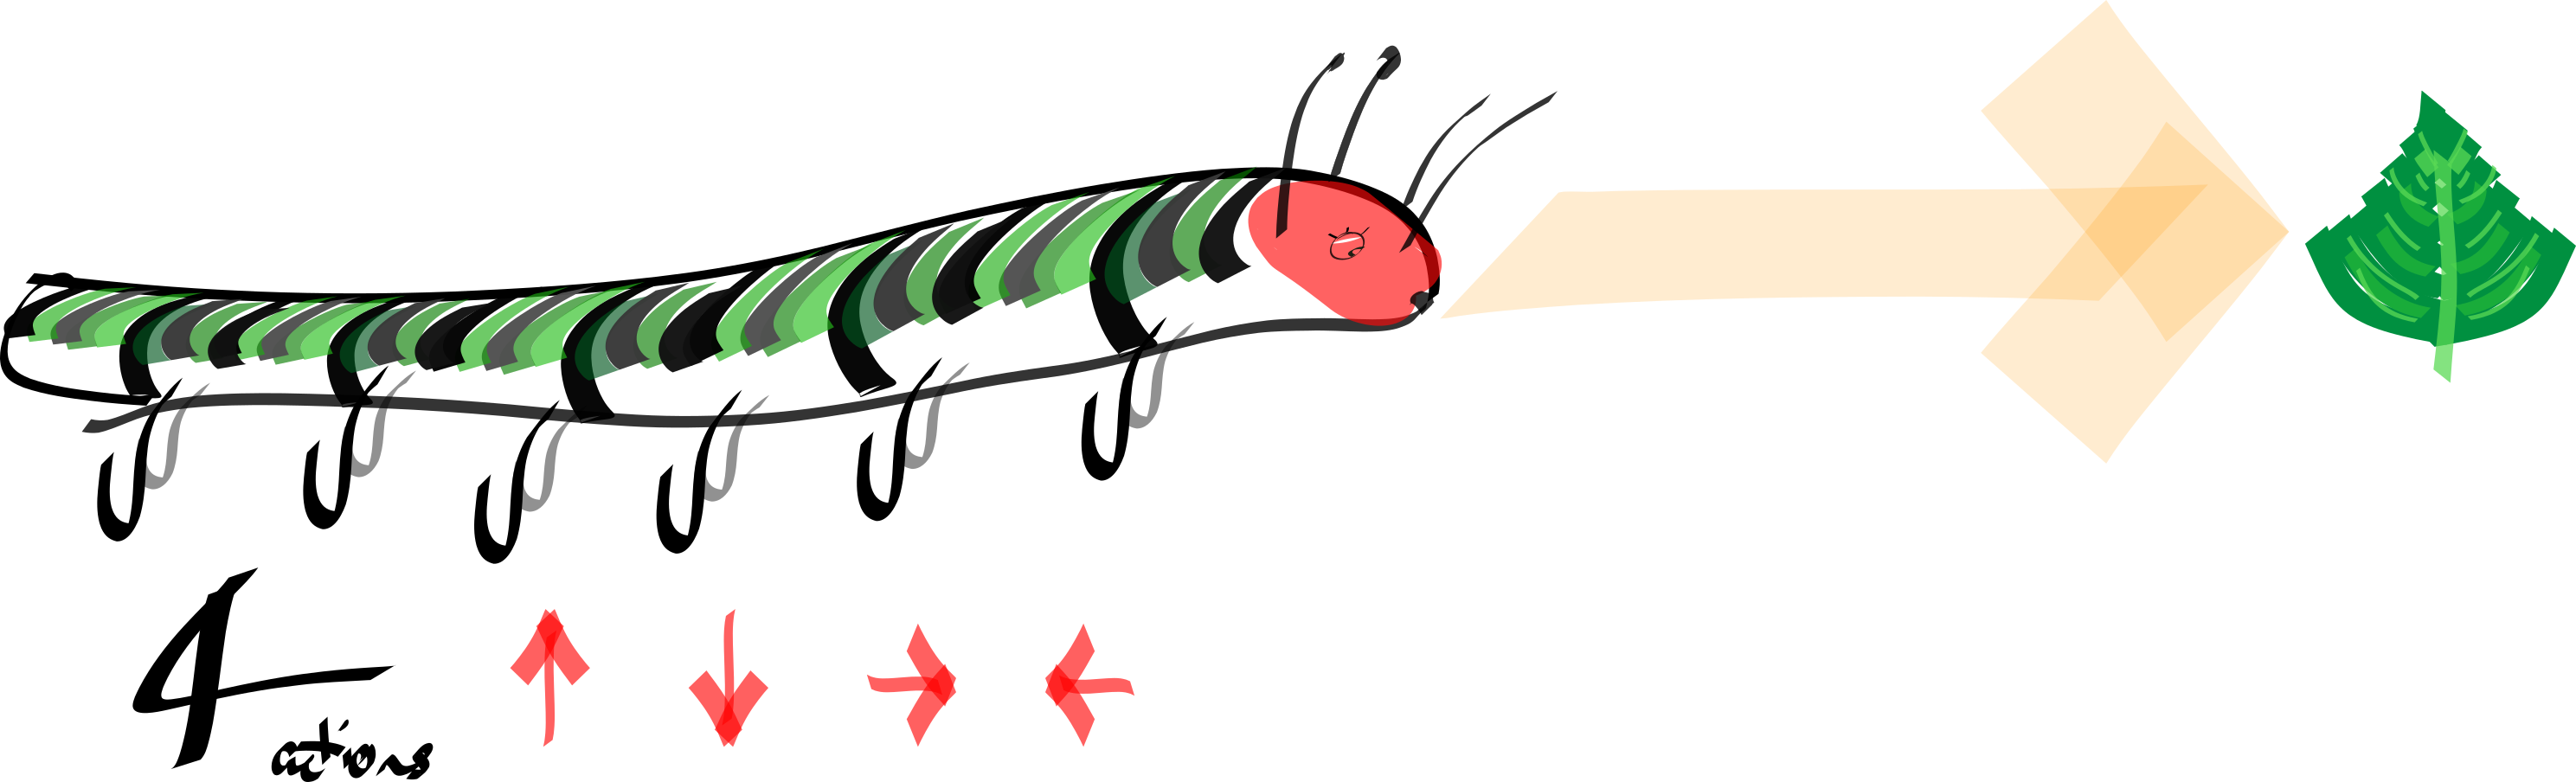
\includegraphics[width=\textwidth,height=0.25\textheight]{../../pictures/drawings/full-caterpillar.png}
\caption{But, what if it could specify actions in another way? Rather than specifying leg movements, it could pick a direction to move, which would specify a program of leg movements.}
\end{figure}


% \begin{figure}
% \centering
% \includegraphics[width=0.5\textwidth,height=0.5\textheight]{../../pictures/figures/discrete-interface.png}
% \caption{The optimisation dynamics of value iteration versus parameterised value iteration.}
% \end{figure}


\subsection{Related work}

\cite{Nagabandi2019}


\chapter{Related work}

How do the topics considered in this thesis relate to the work done in the wider scientific community? Which work uses similar tools, which works build on the same foundations, which works have the same goals?

\hypertarget{related-work}{%
\section{Related work}\label{related-work}}

\hypertarget{mdps}{%
\paragraph{MDPs}\label{mdps}}

Dynamic programming, linear programming, \ldots{}?

\[
Q^{\pi}(s_0, a_0) = r(s_0, a_0)
+ \gamma \mathop{\text{max}}_{a_1} \mathop{\mathbb E}_{s_1\sim p(\cdot | s_0, a_0)} \Bigg[ r(s_1, a_1)
+ \gamma \mathop{\text{max}}_{a_2} \mathop{\mathbb E}_{s_2\sim p(\cdot | s_1, a_1)} \bigg[r(s_2, a_2)
+ \gamma \mathop{\text{max}}_{a_3} \mathop{\mathbb E}_{s_3\sim p(\cdot | s_2, a_2)} \Big[
\dots \Big] \bigg] \Bigg]
\]

\hypertarget{hrl}{%
\subparagraph{HRL}\label{hrl}}

Temoral abstractions of actions.(how does this related to a
decomposition of rewards) Ok, so we wany a multiscale representation?
Understanding how actions combine (this is necessary knowledge for HRL?)

Reasons to do HRL??? (want to verify these claims - and have refs for
them)

\begin{itemize}
\item
  credit assignment over long time periods (learning faster in one env)
\item
  exploration
\item
  transfer
\item
  To learn action abstractions they must capture info about the model.
  How much harder is it to learn action abstractions in model-free vs
  model-based settings?
\item
  Reward as a function of a subspace of the state space. (this is
  important for learning abstract representations and actions!?)
\item
  What do cts linear heirarchical actions look like!? and their loss
  surface!?
\item
  HLMDPs \cite{Saxea}
\item
  Modulated policy heirarchies \cite{Pashevich}
\item
  Model free representations for HRL \cite{Rafati}
\item
  \href{https://blog.aqnichol.com/2019/04/03/prierarchy-implicit-hierarchies/}{Prierarchy:
  Implicit Hierarchies}
\item
  Options
\item
  Near optimal representation learning for heirarchical RL \cite{Nachum2018}
\end{itemize}

Relation to pretraining / conditioning?

\begin{center}\rule{0.5\linewidth}{\linethickness}\end{center}

Why does Heirarchy (sometimes) work so well in reinforcement learning?

The authors claim that the benefits of HRL can be explained by better
exploration. However, I would interpret their results as saying; ``for
2D environments with walls, larger steps / actions result in greater
explration''. But what if the walls were replaced by cliffs? I imagine
this algorithm would do a lot worse!?

They also seem to misunderstand the main problem with HRL, discovery.
Once you have discovered a nice set of abstracted actions / a
representation, then yeah, you get faster reward propagation, better
exploration, \ldots{} etc.

\hypertarget{dynamic-programming}{%
\paragraph{Dynamic programming}\label{dynamic-programming}}

What is it? Memoized search. Why should we care?

\hypertarget{model-based-rl}{%
\subsection{Model-based RL}\label{model-based-rl}}

Pros and cons.

Model-based learning can be bad\ldots{} There may be many irrelevant
details in the environment that do not need to be modelled. A model-free
learning naturally ignores these things.

The importance of having an accurate model!

For example, let \(S\in R^n\) and \(A\in [0, 1]^n\). Take a transition
function that describes how a state-action pair generates a distribution
over next states \(\tau: S \times A \to \mathcal D(S)\). The reward
might be invariant to many of the dimensions.
\(r: X \times A -> \mathbb R\), where \(X \subset S\).

Thus, a model mased learner can have arbitrarily more to learn, by
attempting to learn the transition function. But a model-free learner
only focuses on \ldots{}

This leads us to ask, how can we build a representation for model-based
learning that matches the invariances in the reward function. (does it
follow that the invariances in reward fn are the invariances in the
value fn. i dont think so!?)

Take \(S \in R^d\) and let \(\hat S = S \times N, N \in R^k\). Where
\(N\) the is sampled noise. How much harder is it to learn
\(f: S \to S\) versus \(\hat f: \hat S \to \hat S\)?

https://arxiv.org/pdf/1903.00374v3.pdf https://arxiv.org/abs/1907.02057

\hypertarget{representation-learning-and-abstraction}{%
\subsection{Representation learning and
abstraction}\label{representation-learning-and-abstraction}}

The goal is to find a representation that decomposes knowledge into its
parts.

Another way to frame this is: trying to find the basis with the right
properties.

\begin{itemize}
\tightlist
\item
  sparsity,
\item
  independence,
\item
  multi scale,
\item
  locality/connectedness
\item
  ???
\end{itemize}


Types of abstraction for RL. Abstraction for efficient;

\begin{itemize}
\tightlist
\item
  exploration, [Learning latent state representation for speeding up exploration](https://arxiv.org/abs/1905.12621)
\item
  optimal control,
\item
  ???,
\end{itemize}


\subsection{Heirarchical reinforcement learning}


\chapter{Final remarks}\label{C:con}

\section{Summary}

While there do exist some tools for analysing abstractions for RL, we need better ones.
There are many unanswered questions (below), but, most importantly,
there is no well defined way to evaluate abstractions in general. {\color{red} doesnt quite work}

Linear Markov Decision Problems attempt to preserve the space of transition dynamics and the rewards.
But, they failed to preserve the value of the optimal actions, and thus cannot
guarantee performance in general. Ultimately, this was because the Bellman equation is non-linear.

We develop a measure of symmetry, and use it to give reinforcement learners a preference towards symmetry, a prior.
Our results did not show any advantage by using this prior, but due to computational and temporal\footnotemark constraints,
we were unable to make any conclusions.
% Symmetry attempts to preserve, ...?

\footnotetext{Temporal constraints meaning: A masters is a finite amunt of time.}

\newpage
\section{Future work}

There is a large amount of future work to be done if we want to:

\begin{displayquote}
\textit{understand how abstractions can increase the efficiency of reinforcement learning.}
\end{displayquote}

Our exploration of \textbf{Abstractions} in \ref{abstraction-rl}, raises a few fundamental questions;

\begin{itemize}
	\tightlist
	\item What is the advantage, if any, of \textit{state and action abstraction} versus \textit{state-action abstraction} \ref{exploit-abstraction-rl}?
	\item Of the two approaches to temporal abstraction, \textit{goal-like} and \textit{option-like} temporal abstraction, is one strictly better that the other? If not, then in which cases does \textit{goal-like} temporal abstraction perform better?
	\item Are the facets of evaluation presented in \ref{eval-abstractions} necessary and / or sufficient for 'efficient' performance of an abstraction in practice?
	\item Do many, or even all, abstractions of interest to RL live in the family defined in \ref{similar-classes}?
	\item Is there a difference between trajectory based similarity measures (that set the similarity $\chi(x, x')$ to be built from distances between the cumulants $D(c(x, \pi), c(x', \pi))$, rather than expected discounted cumulants $D(\mathcal C(x, \pi), \mathcal C(x, \pi))$)?
	\item What is the trade off (between computation and approximation error) of approximating $\int_{\pi \in \Pi}f(\pi)$ with $B \subset \Pi, \; \int_{\pi \in B}f(\pi)$?
	% How large does $X$ need to be to get a reliable estimate? Can we pick $X$ in intelligent, or random ways.
	\item What is necessary (rather than sufficient - which is proved in existing work) for the preservation of Bellman equation's ability to guide search? Can we weaken the requirements to: preserving the ordering of the value of optimal actions (rather than their absolute values as in existing work)?
\end{itemize}

Similarly, our results on \textbf{LMDPs} \ref{lmdp-validation} leave a few questions unanswered;

\begin{itemize}
	\tightlist
	\item In which cases does the LDMP give the right solution?
	\item What are the properties that make a MDP easily solvable (via LDMPs)?
	\item Can easily solvable MDPs (via LDMPs) be easily identified?
\end{itemize}

Finally, our results on \textbf{symmetric abstractions} \ref{symmetric-abstractions} leave a few questions unanswered;

\begin{itemize}
	\tightlist
	\item What is the (computational) efficiency of rejection sampling for symmetry biased distributions, and how does it scale with dimension? And how much data (sample efficiency) does that computation buy?
	% \item Rather than rejection sampling, use Metropolis-hastings. To allow to scale to higher dimensions.
	\item What happens if we use our measure of symmetry \ref{measure-symmetry} as a regulariser (as it is differentiable)?
	\item Invariants ...
	\item How can representations of states (or state-actions or ...) be ordered or structured? And how does this structure reduce the combinatorial space of possible symmetries?
	\item What is the cost of discovering temporal symmetries? How does this cost scale with the length of time? Can we amortize this cost by building symmetries from smaller symmetries in shorter sequences?
	% \item Run more rigorous experiments...
\end{itemize}

% % % % % % % % % % % % % % %
% Q: Number of integer factors as a function of n???
% Q: Efficiency of rejection sampling.
% Q: Relation to Lyapanov dynamics. Sampling distributions with gradient descent!??!
% Q: Proximity to symmetric states. How does this change as d increases?
% Q: Is there an advantage to building your temporal abstraction from k=n first, then to k=n+1.
% Q: Metro hastings. == RL?!? Pick transitions to help estimate a distribution?
% Q: With increasing k, does the topology of temporal abstractions always get coarser?



%%%%%%%%%%%%%%%%%%%%%%%%%%%%%%%%%%%%%%%%%%%%%%%%%%%%%%%

% and of course book style knows about backmatter
% \backmatter caused problems with appendices :-(
% and of course report style doesn't
%%%%%%%%%%%%%%%%%%%%%%%%%%%%%%%%%%%%%%%%%%%%%%%%%%%%%%%


\bibliographystyle{ieeetr}
% \bibliographystyle{acm}
\bibliography{mendeley}

\appendix

\chapter{MDPs}

\section{Tabular MDPs}\label{vf-neumann}

It is possible to derive the value functional in another, possibly more enlightening way. But it takes a little more work. It requires a result from real analysis, the Neumann series. Which is simply the generalisation of a geometric series to contractive linear operators, such as a matrix.

\begin{align*}
r &\in (-1, 1) \\
(1-r)^{-1} &= \lim_{n\to \infty} \sum_{i=0}^n r^i \tag{Geometric series}\\
T &\in \mathbb X^k: \det(T) \in (-1, 1) \\
(I-T)^{-1} &= \lim_{n\to \infty} \sum_{i=0}^n T^i \label{eq:neumann}\tag{Neumann series}
\end{align*}

We can expand the recursion in the Bellman equation to get an \eqref{eq:inf-series}. We can then use the \eqref{eq:neumann} (by setting $T=\gamma \tau_{\pi}$) to give the nice analytic form of the value functional.

\begin{align*}
V &= r_{\pi} + \gamma \tau_{\pi} V \tag{Bellman eqn}\\
V &= r_{\pi} + \gamma \tau_{\pi}\big( r_{\pi} + \gamma \tau_{\pi} V\big) \\
V &= r_{\pi} + \gamma \tau_{\pi}\Big(r_{\pi} + \gamma \tau_{\pi}\big( r_{\pi} + \gamma \tau_{\pi} V\big)) \\
&= r_{\pi} + \gamma \tau_{\pi}r_\pi + \gamma^2 \tau_{\pi}\tau_{\pi}r_{\pi} + \gamma^3 \tau_{\pi}\tau_{\pi}\tau_{\pi}V \\
&= \sum_{t=0}^{\infty} \gamma^t\tau_{\pi}^tr_{\pi} \label{eq:inf-series}\tag{infinite series} \\
&= \big( \sum_{t=0}^{\infty} \gamma^t\tau_{\pi}^t \big) \cdot r_{\pi}\\
&= (I-\gamma \tau_{\pi})^{-1} r_{\pi} \tag{value functional}\\
\end{align*}

This proof is more satisfying because we can more clearly see the nature of the value functional. It is a closed form of the infinite sum of discounted future rewards.


\section{Policies in high dimensions}\label{high-D-policies}

Let's \textit{try} to gain intuition about the space of policies in higher dimensions.
For each state, we have a distribution (on a simplex), over the possible actions.

Imagine what the geometry of the space of policies in the two state, two action MDP. A policy tells us which actions should be taken when in a given state. Therefore, there will be \(|A| \times |S|\) entries in the policy. However, because the policy returns a distribution over actions, the true dimensionality of the policy is \((|A| -1) \times |S|\). Which in the two state, two action case equals 2D.

\begin{figure}[h]
\centering
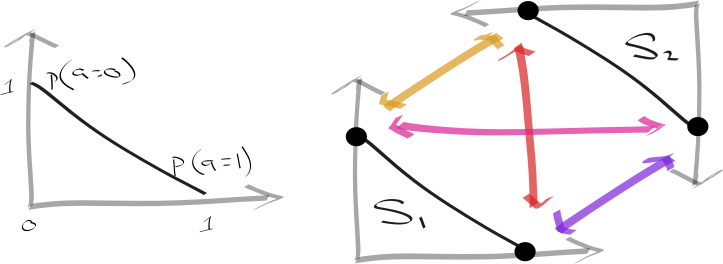
\includegraphics[width=1\textwidth,height=0.20\textheight]{../../pictures/drawings/2-state-2-action-simplices.png}
\caption{(left) Given that you are in state, $s$, we have a simplex over two actions $\{a_1, a_2\}$.
(right) The policy must describe distributions over actions for each state,
so the policy space must describe the $|S|$ possible combinations of distribution over actions.}
\end{figure}

\begin{figure}[h]
\centering
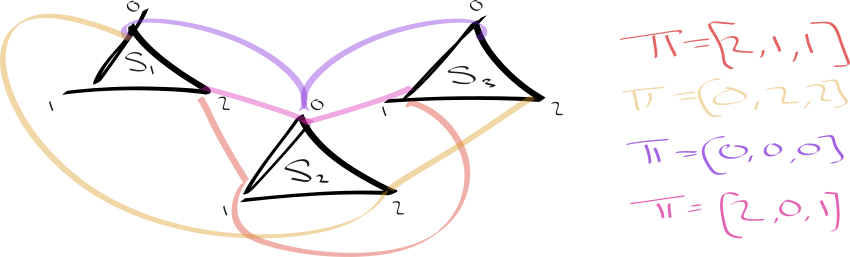
\includegraphics[width=1\textwidth,height=0.25\textheight]{../../pictures/drawings/3-state-3-action-simplices.png}
\caption{Here we are visualising the policy space of a three state, three action, MDP.
For each state, we must specify a distribution over actions.}
\end{figure}

\newpage

\section{Other properties of the polytope} \label{polytope-extras}



\subsection{Distribution of policies}

A potentially interesting question to ask about the value polytope is how the
values (of the policies) are distributed. we can calculate this
density analytically by using the probability chain rule:
\(p(f(x)) = \mid \det\frac{\partial f(x)}{\partial x}\mid^{-1}p(x)\).
Where we set \(f\) to be our value functional and \(p(x)\) to be a
uniform distribution over policies. Thus we have;

\begin{align}
p(V(\pi)) = |\det \frac{\partial V(\pi)}{\partial \pi}|^{-1} \cdot p(\pi) \tag{density}
\end{align}

\begin{figure}
\centering
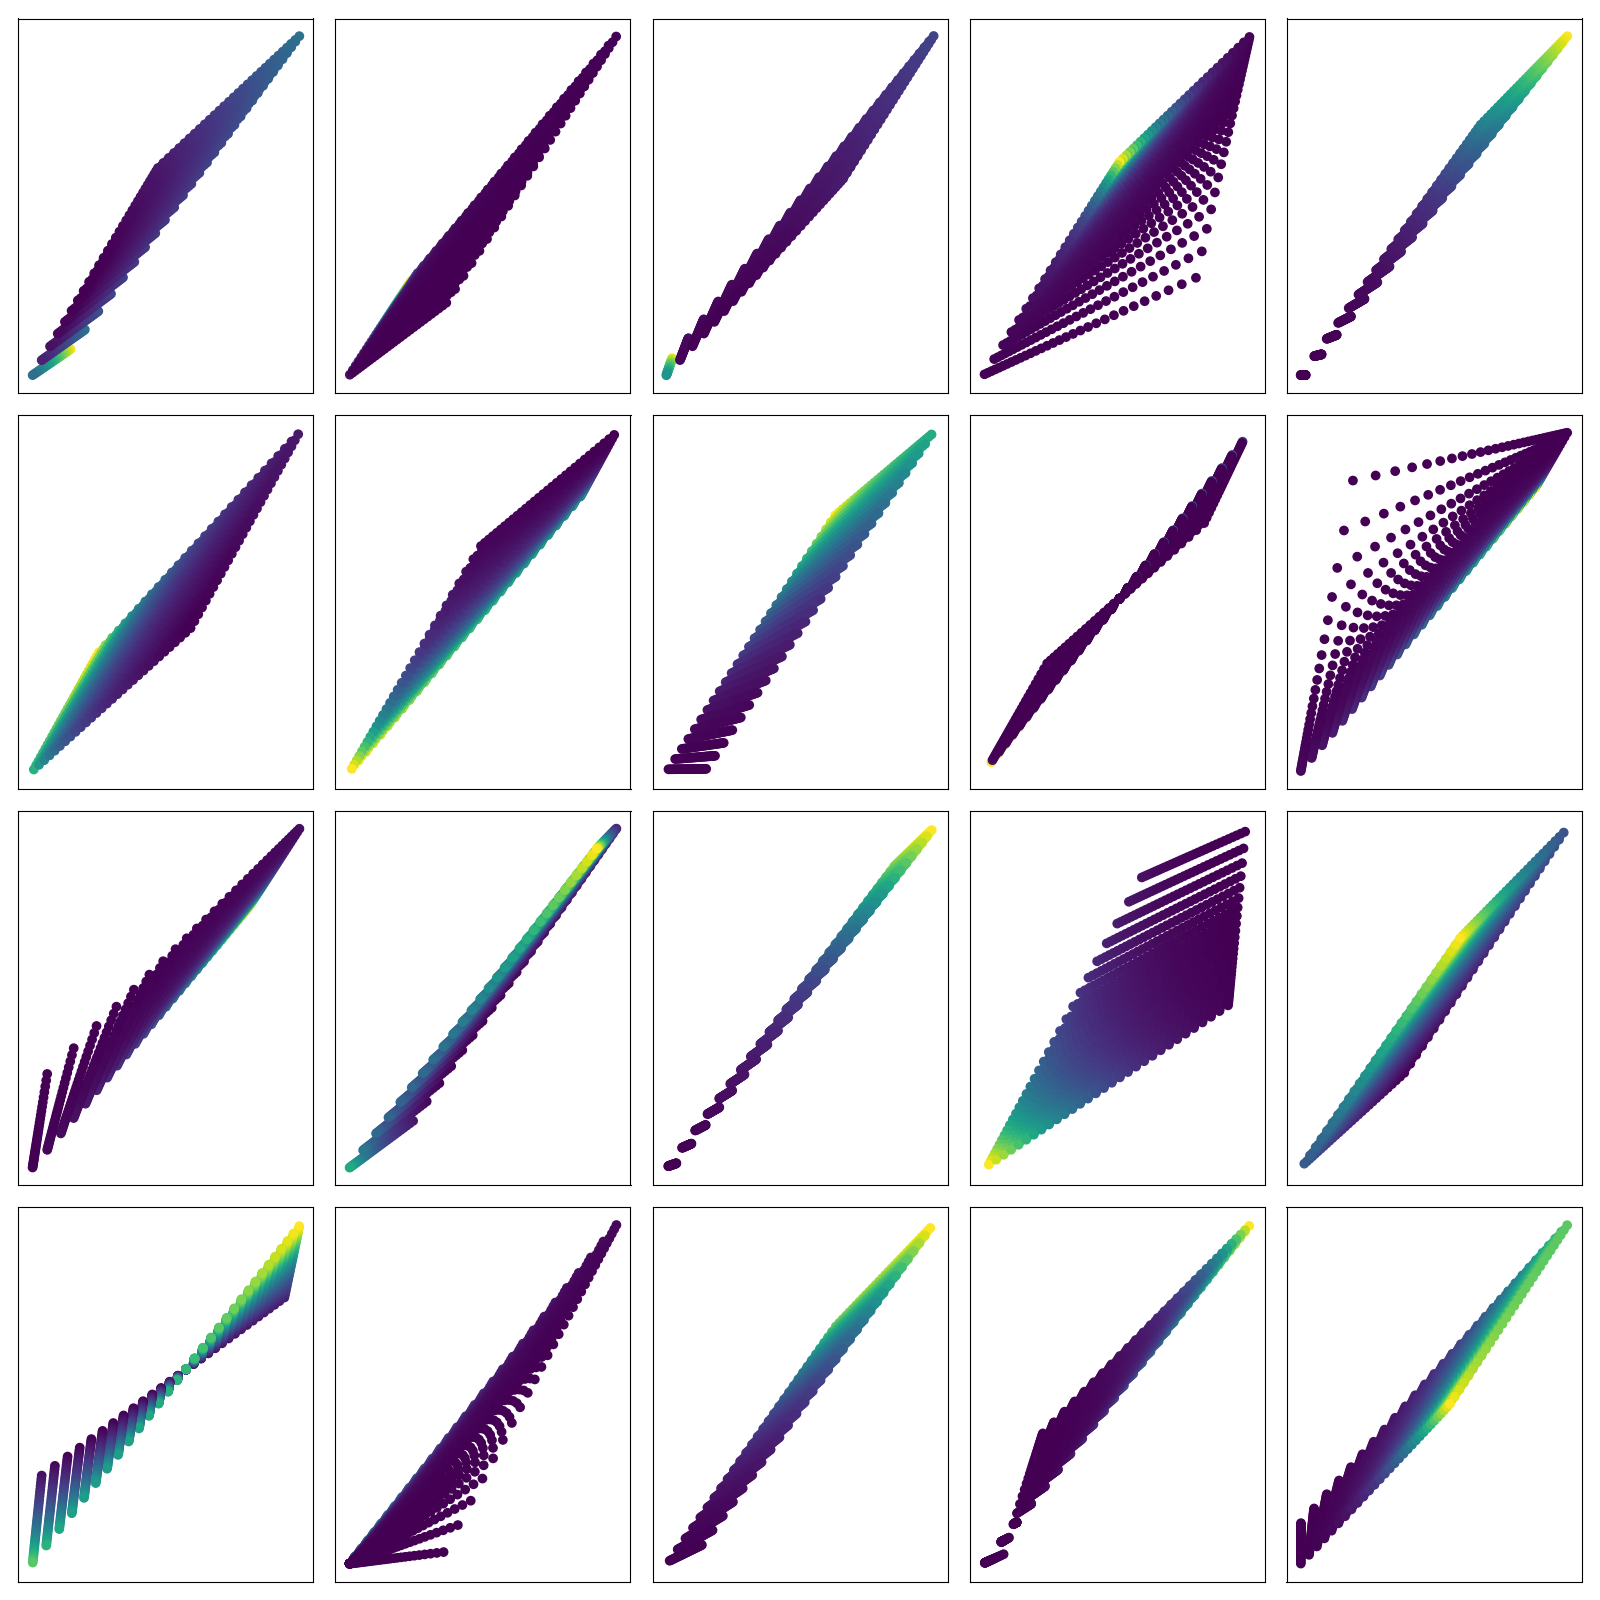
\includegraphics[width=1\textwidth,height=1\textheight]{../../pictures/figures/polytope_densities.png}
\caption{Here we have visualised the value polytope for 2-state 2-action MDPs. They are colored by the likelihood of
each value under a uniform distribution over policies.
Lighter color is higher probability.}
\label{fig:density}
\end{figure}

As we can see in \ref{fig:density}: for some polytopes, there is high density around the optimal policy.
In other polytopes, many of the policies are far away from the optimal policy.

Consider the expected suboptimality of our MDP, which tells us how far away the
optimal policy is from the 'center of value' of the polytope.

\begin{align*}
\mu_M(s) &:= \mathop{\mathbb E}_{\pi\sim\Pi}\Big[V_M^{\pi}(s) \Big]\\
\epsilon^{* }(M) &= \mathop{\text{max}}_s V_M^{\pi^{* }}(s) - \mu(M)(s)
\end{align*}

This suggests that MDPs with low expected suboptimality, $\epsilon^{* }(M)$, are easier to solve than other MDPs.
This is because we can simply sample a random policy which is likely to be close to the optimal policy
(or we could sample many policies and pick the best, which would, with high probability, be close(r) to the optimal policy).

\vspace{5mm}

\textbf{Open problem}\footnotemark: If an MDP has sub-optimality,  $\epsilon^{* }(M)$,
then it is possible to find a $\epsilon$ optimal policy with $\{\}$ samples.

\footnotetext{Open problem* of dubious interest.}

Where $\epsilon = \mathop{\text{max}}_s V^{\pi^{* }}(s) - V(s)$.

\vspace{5mm}

However, this strategy will not scale to higher dimensions.
As we increase the state size or action size, the chance that there is high
density near the optimal policy (or a randomly sampled MDP) decreases with rate proprtional to $|A|^{|S|}$.

% \textbf{Experiment:} Correlate the properties of \(P, r\) with entropy.
% Or find derivative wrt \(P, r\). What properties of \(P, r\) yield
% easily solvable MDPs?

\subsection{Discounting}

Another question you may have is: \textit{how does the shape of the polytope depend on the discount rate?}
Given an MDP, we can vary the discount rate from \(0\) to \(1\) and visualise
the shape of the value polytope.

\begin{figure}
\centering
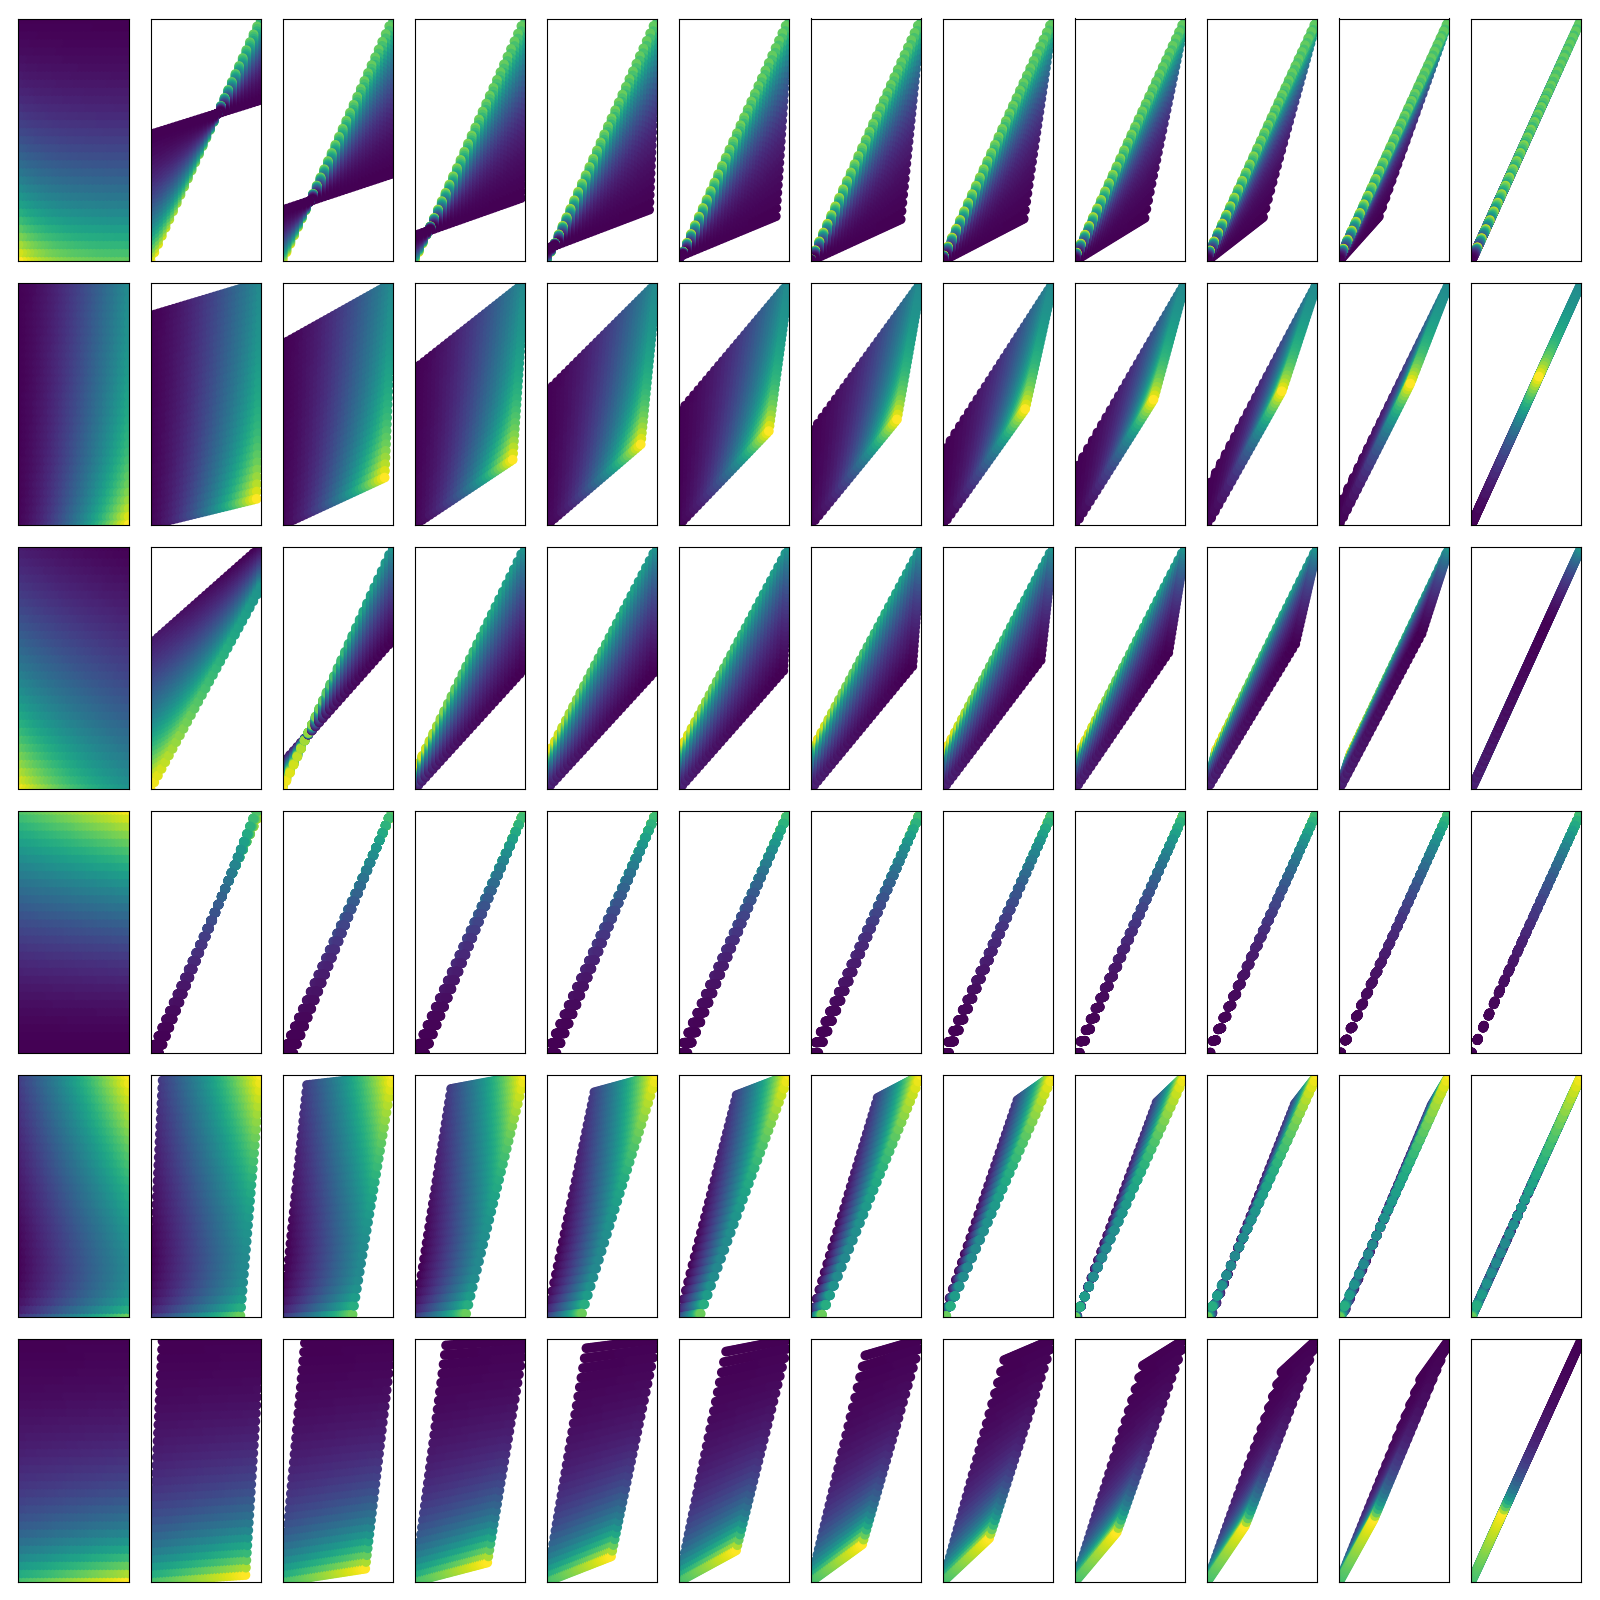
\includegraphics[width=1\textwidth,height=1\textheight]{../../pictures/figures/discounts.png}
\caption{Here we have visualised the value polytope for 2-state 2-action MDPs. The
rows show how their value polytopes change with changes in discount rate, ranging linearly from 0 (left), to 1 (right).
The color map is represents the density of policies, as in \ref{fig:density}.}
\label{fig:polytope-discounts}
\end{figure}

As we can see in \ref{fig:polytope-discounts}. As the discount rate tends to $1$,
all the policies are projected into a 1D space. (is this 1D for 2D problems. is it always 1D?)

\subsection{Derivation of derivative}

We want to derive the derivative of the value functional. Here we go.

\begin{align*}
V(\pi) &= (I − \gamma \tau_{\pi})^{−1}r_{\pi} \tag{value functional}\\
&= (I − \gamma \tau\cdot \pi)^{−1}r\cdot \pi \\
\frac{\partial V}{\partial \pi} &= \frac{\partial}{\partial \pi}((I-\gamma \tau_{\pi})^{-1} r_{\pi}) \\
&= (I-\gamma \pi \tau)^{-1} \frac{\partial \pi r}{\partial \pi}+   \frac{\partial (I-\gamma \pi \tau)^{-1}}{\partial \pi}\pi r\tag{product rule} \\
&= (I-\gamma \pi \tau)^{-1} r + -(I-\gamma \pi \tau)^{-2} \cdot -\gamma \tau\cdot \pi r\\
&= \frac{r}{I-\gamma \pi \tau} + \frac{ \gamma \tau\cdot \pi r}{(I-\gamma \pi \tau)^2} \tag{rewrite as fractions}\\
&= \frac{r(I-\gamma \pi \tau) + \gamma \tau \pi r}{(I-\gamma \pi \tau)^2} \tag{common demoninator}\\
& = \frac{r}{(I-\gamma \tau \pi)^2} \tag{cancel}
\end{align*}

\newpage
\section{Model search} \label{model-iteration}

As noted in \ref{search-spaces-mdps}, we can search through policy space or value
space, each with their own structure.
There is a third search space we could consider, the model parameters.

However, this problem is not a control problem like the search for values or policies.
This is an inference problem, we are trying to infer the model parameters.
Once we know these parameters, we can apply control.
In general, this is known as model-based RL.

We could search through models ($\tau, r$) using supervision from next step prediction.
This is a common approach to model-based RL \cite{Wang2019a}.
Rather, we consider using the value estimation error to guide the search for model parameters.

\begin{align}
\tilde P^{* }, \tilde r^{* } = \mathop{\text{argmin}}_{\tilde \tau, \tilde r} \int_{\Pi} \parallel V_{\tau, r}(\pi)-V_{\tilde \tau, \tilde r}(\pi) \parallel_\infty
\end{align}

\begin{figure}
\centering
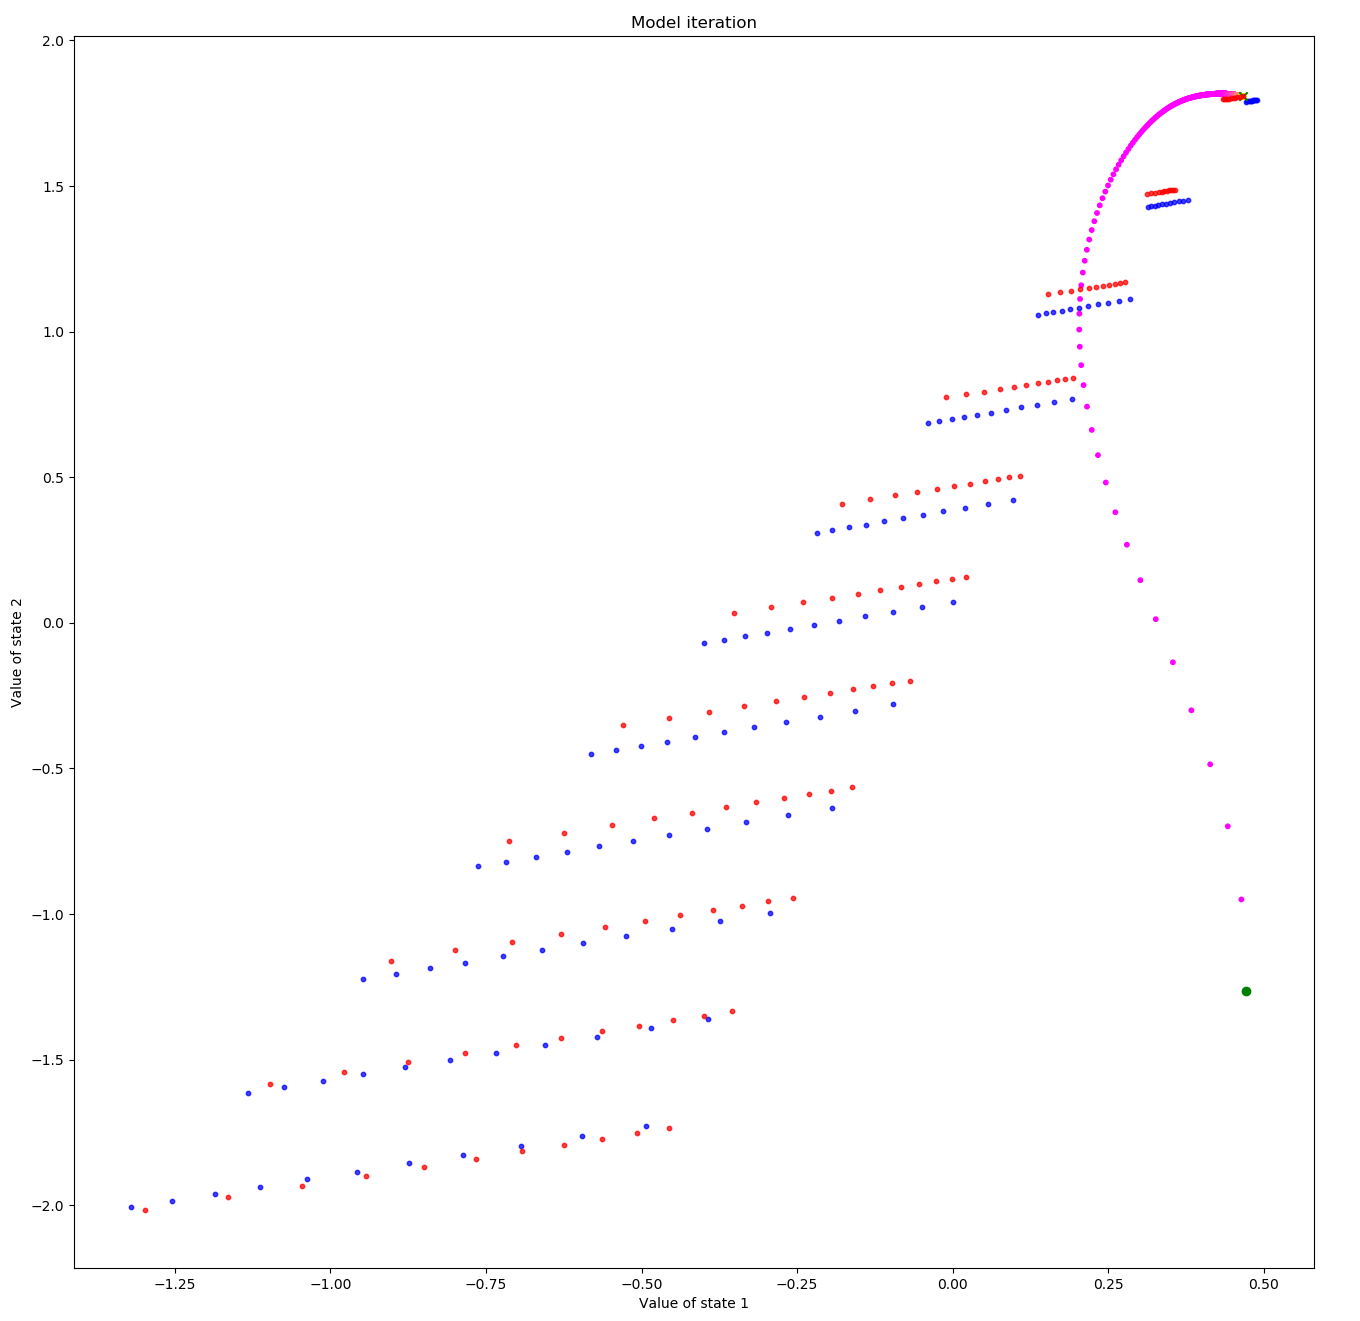
\includegraphics[width=1.0\textwidth,height=0.8\textheight]{../../pictures/figures/model_iteration.png}
\caption{Model iteration applied to a 2-state, 2-action MDP.
Blue shows the value of policies when evaluated under the true model, $\tau, r$,
and Red shows the estimated value of policies when evaluated under the learned model at convergence, $\tilde \tau, \tilde r$.}
\end{figure}

There is a main advantage and some disadvantages to this framework.
The advantage is that this approach focuses its resources only on 'relevant' features of the model.
The disadvantages are that it requires many policy evaluations (from the environment),
and many estimates of a policy's value (simulated evaluations).

\subsection{Relevant features of the model}

Model iteration via value prediction error only focuses on 'relevant' features of the model \footnotemark.
Relevant in the sense that they are useful for accurately predicting state values.

\footnotetext{Model free approaches to RL also focus on 'relevant' features, however, they do not explicitly represent the underying model.}

Consider a problem where the reward is only determined by the first feature of the state.
We can add arbitrarily many extra features. A model-based learner that learns through next step prediction will attempt to
accurately predict all of these features. This unnecessarily spends resources.

More formally; let the state space but a subset of the reals $S \subset \mathbb R^d$.
And construct a reward function that is only dependent on the first feature of the state space, $r(s, a) = f(s^0, a)$.
While the transition function is constructed so that, there exists a $k$ dimensional subspace (that includes the first feature)
that is independent of the other $d-k$ features, $\tau(s'|s, a) = [g_1(s^{0:k}, a), g_2(s^{k:d}, a)]$.

An example with this structure, could be the addition of $d-k$ 'noise' features,
that play no part in the transition dynamics, but only describe inessential features
(such as features that describe the positions of leaves on a windy day).

% \subsection{Jokes}
%
% This is just a less intelligent reinvention of Thompson sampling for MDPs.
% No it isnt?!? They use

\subsection{Policy evaluations}

We receive $V_{P, r}(\pi)$ from the environment. But we want to minimise the number
of these calls to the environment, as it can be expensive to evaluate a policy with high accuracy.

Also, for each iteration of $\tilde \tau_t, \tilde r_t$, we need to estimate the
value of many policies, $\forall \pi; V_{\tilde \tau_t, \tilde r_t}(\pi)$. This requires lots of compute.

Rather than integrating over all policies (thus requiring us to evaluate all of them),
we only need the deterministic policies. As, Bellamare et al. 2019 show that \textit{"the maximal approximation error
measured over all value functions is the same as the error measured over the set of extremal vertices [aka deterministic policies]"}\cite{Bellemare2019b}.
However, this still requires us to evaluate $|A|^{|S|}$ policies, and to simulate $T |A|^{|S|}$ policies. \footnotemark

% maybe a connction to compressed sensing?!
\footnotetext{It should be possible to use off policy estimation techniques to further reduce the required samples / compute. But we leave this for future work.}

\newpage
\section{Visualising higher dimensional MDPs}\label{graph-vis}

So this value polytope works well for 2D. And could be extended to 3D. But, what about higher dimensions?

\begin{displayquote}
  \textit{"To deal with a 14-dimensional space, visualize a 3-D space and say 'fourteen' to yourself very loudly. Everyone does it."} Geoff Hinton
\end{displayquote}

Is there intuition we might gain from visualising optimisation on MDPs with the
number of states and / or actions being greater than 3?

How to construct them? Decompose the value of a policy as a convex combination
of the values of the deterministic policies.

\begin{align*}
  \alpha(\pi) = \mathop{\text{argmin}}_{\alpha \in \Delta^n} \parallel  V(\pi) - \sum_i (V(\pi_i) \cdot \alpha_i ) \parallel_2^2 + H(\alpha)
\end{align*}

The entropy term ensures we prefer convex combinations with lower entropy.
% Properties of the graphs / graph signals?
\newpage

\begin{figure}[!h]
\centering
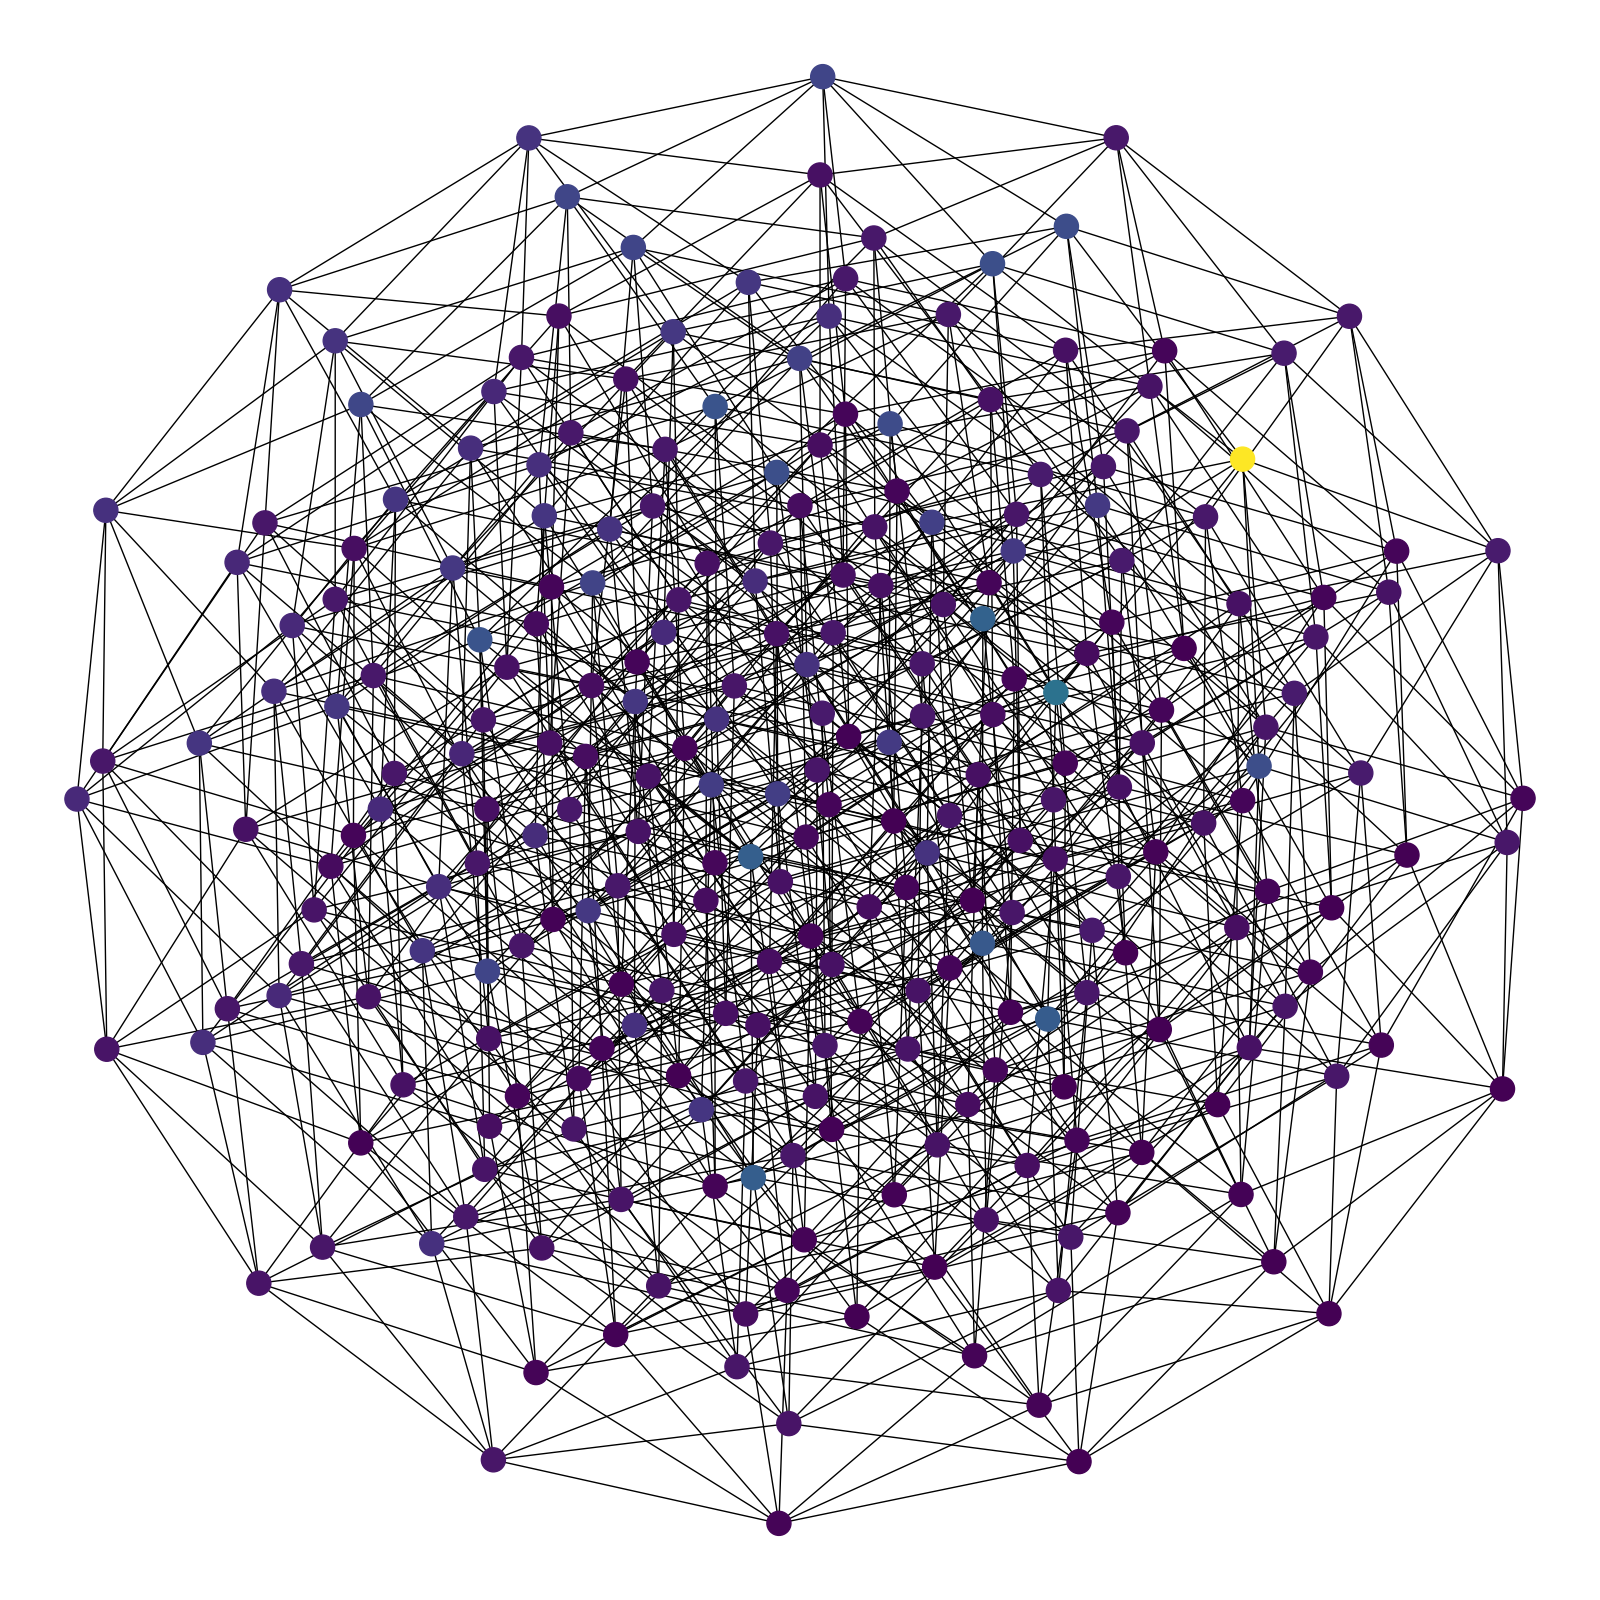
\includegraphics[width=0.5\textwidth,height=0.3\textheight]{../../pictures/figures/discrete-graph.png}
\caption{PI bounces between the nodes of the graph.
So the search of the optimal policy using PI can be visualised as the walk along a graph.
Note: the current policy is shown in yellow (close to the top right).}
\end{figure}

% As each node is a deterministic policy.
% Thus policy iteration is equivalent to finding the shortest path on a XX connected policy graph.

\begin{figure}[!h]
\centering
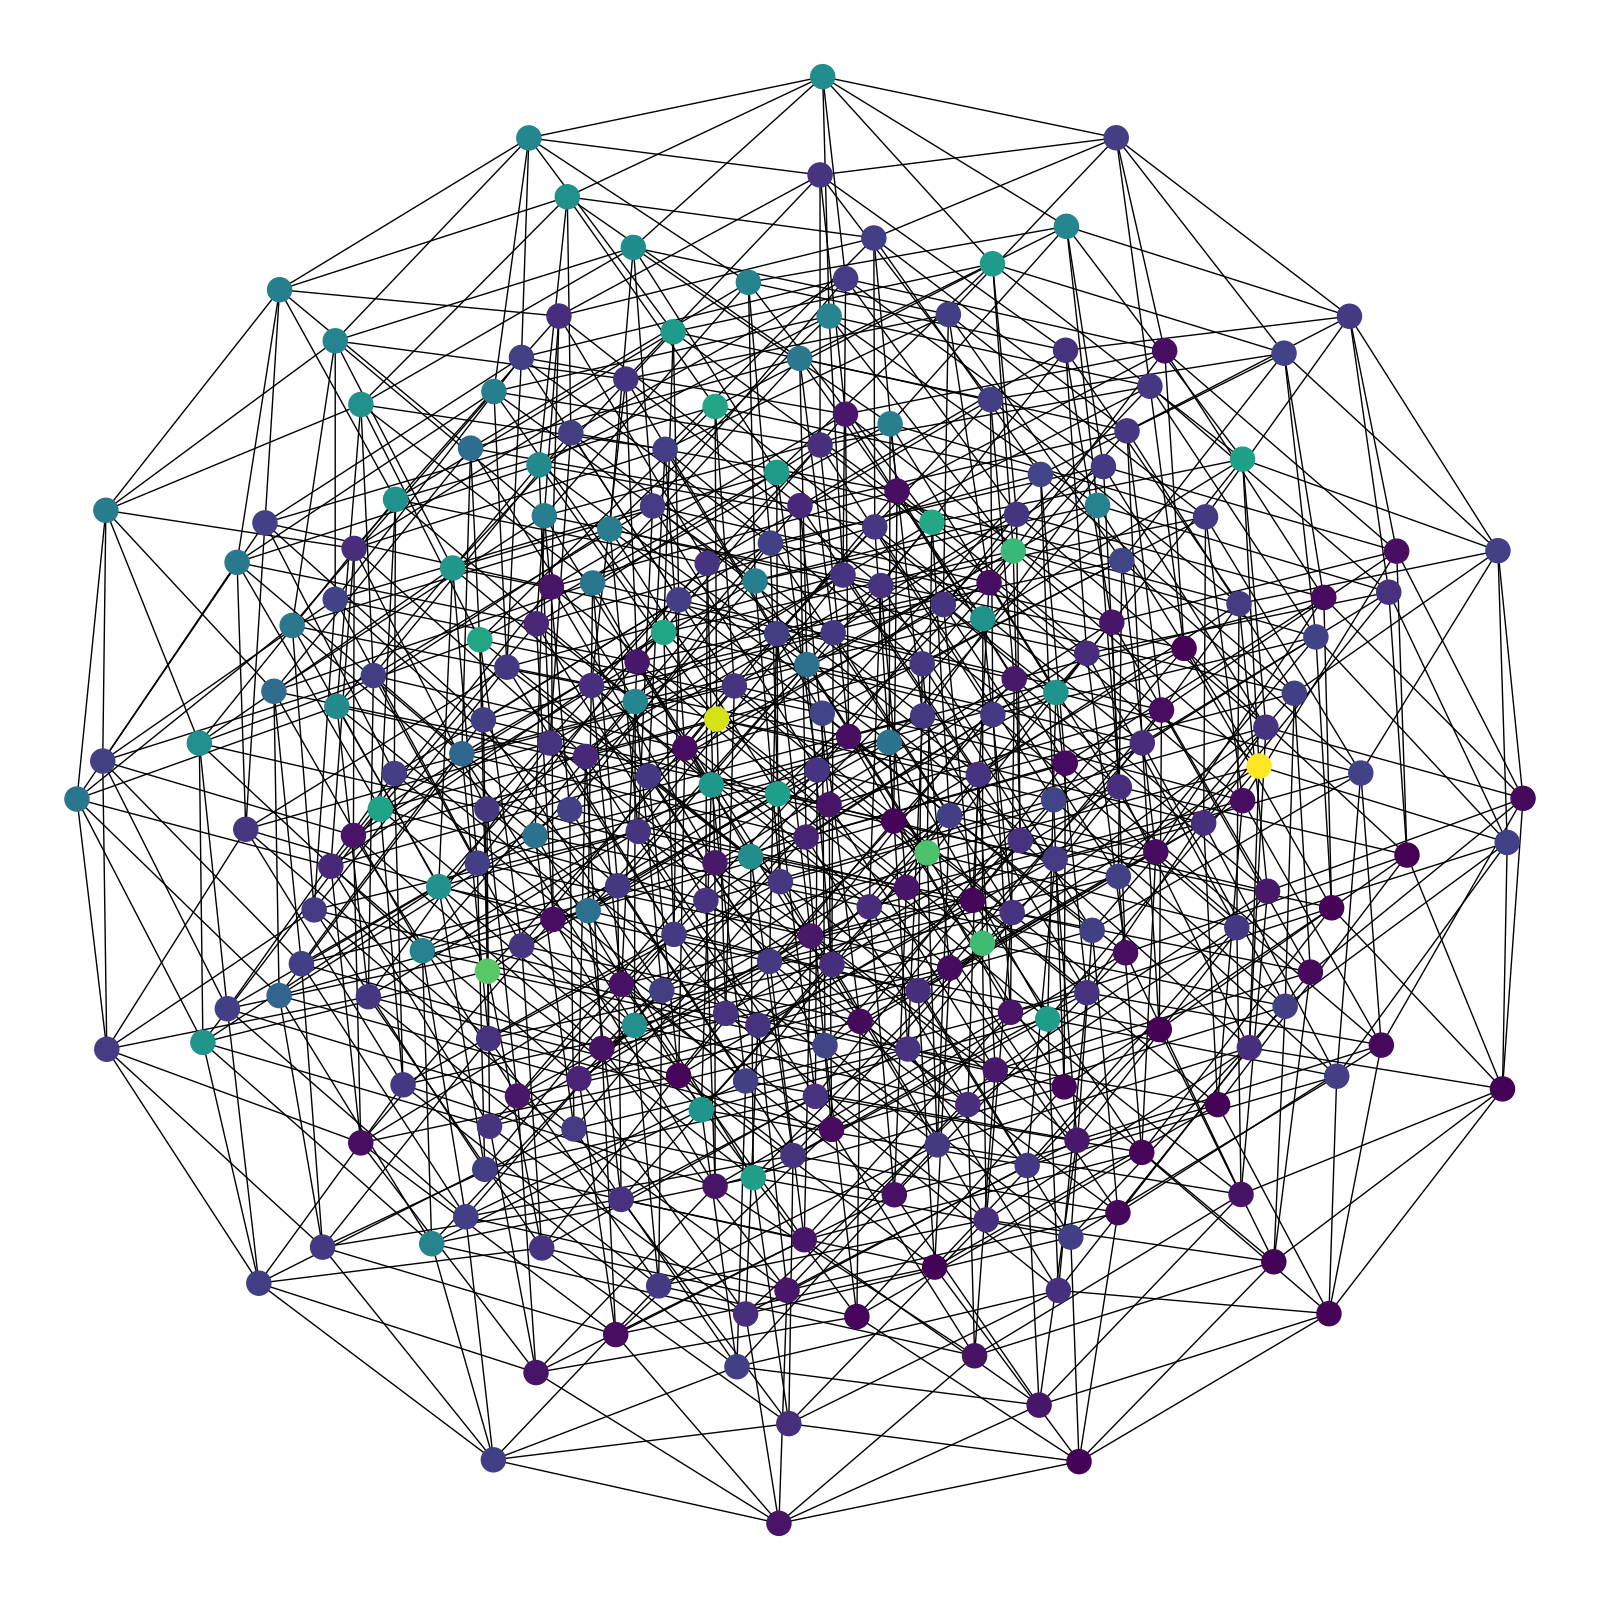
\includegraphics[width=0.5\textwidth,height=0.3\textheight]{../../pictures/figures/interior-graph.png}
\caption{Policy gradient traverses through non-deterministic policies.
So the search of the optimal policy using PG can be visualised the dynamics of a graph signal.}
\end{figure}


\newpage
\section{Deep policy gradients}\label{ss-extras}

From the search spaces section \ref{search-spaces-mdps}, we are left wondering;

\begin{itemize}
\tightlist
\item In which spaces can we (efficiently) calculate gradients?
\item In which spaces can we do convex optimisation?
\item In which spaces does momentum work (well)?
\end{itemize}

Currently, the most successful deep RL approaches are variants of policy gradient methods \cite{Mnih2016,Schulmanb}.
Despite their efficacy in practice, we still don't have a good understanding of
how policy gradient methods combine with deep learning methods to give performant agents.

A key feature of deep learning is over parameterisation (among the other features;
hierarchies, non-linearity, smoothness, locality). There has been recent work
attempting to understand the effect of overparameterisation \cite{Arora2018}.

Here we explore the effects of;
\begin{itemize}
\tightlist
  \item overparameterising the policy and then using policy gradient methods to find the optimally policy.
  \item reparameterising the loss function, thus yielding some ither space to search through.
\end{itemize}

% \begin{figure}[!h]
% \centering
% 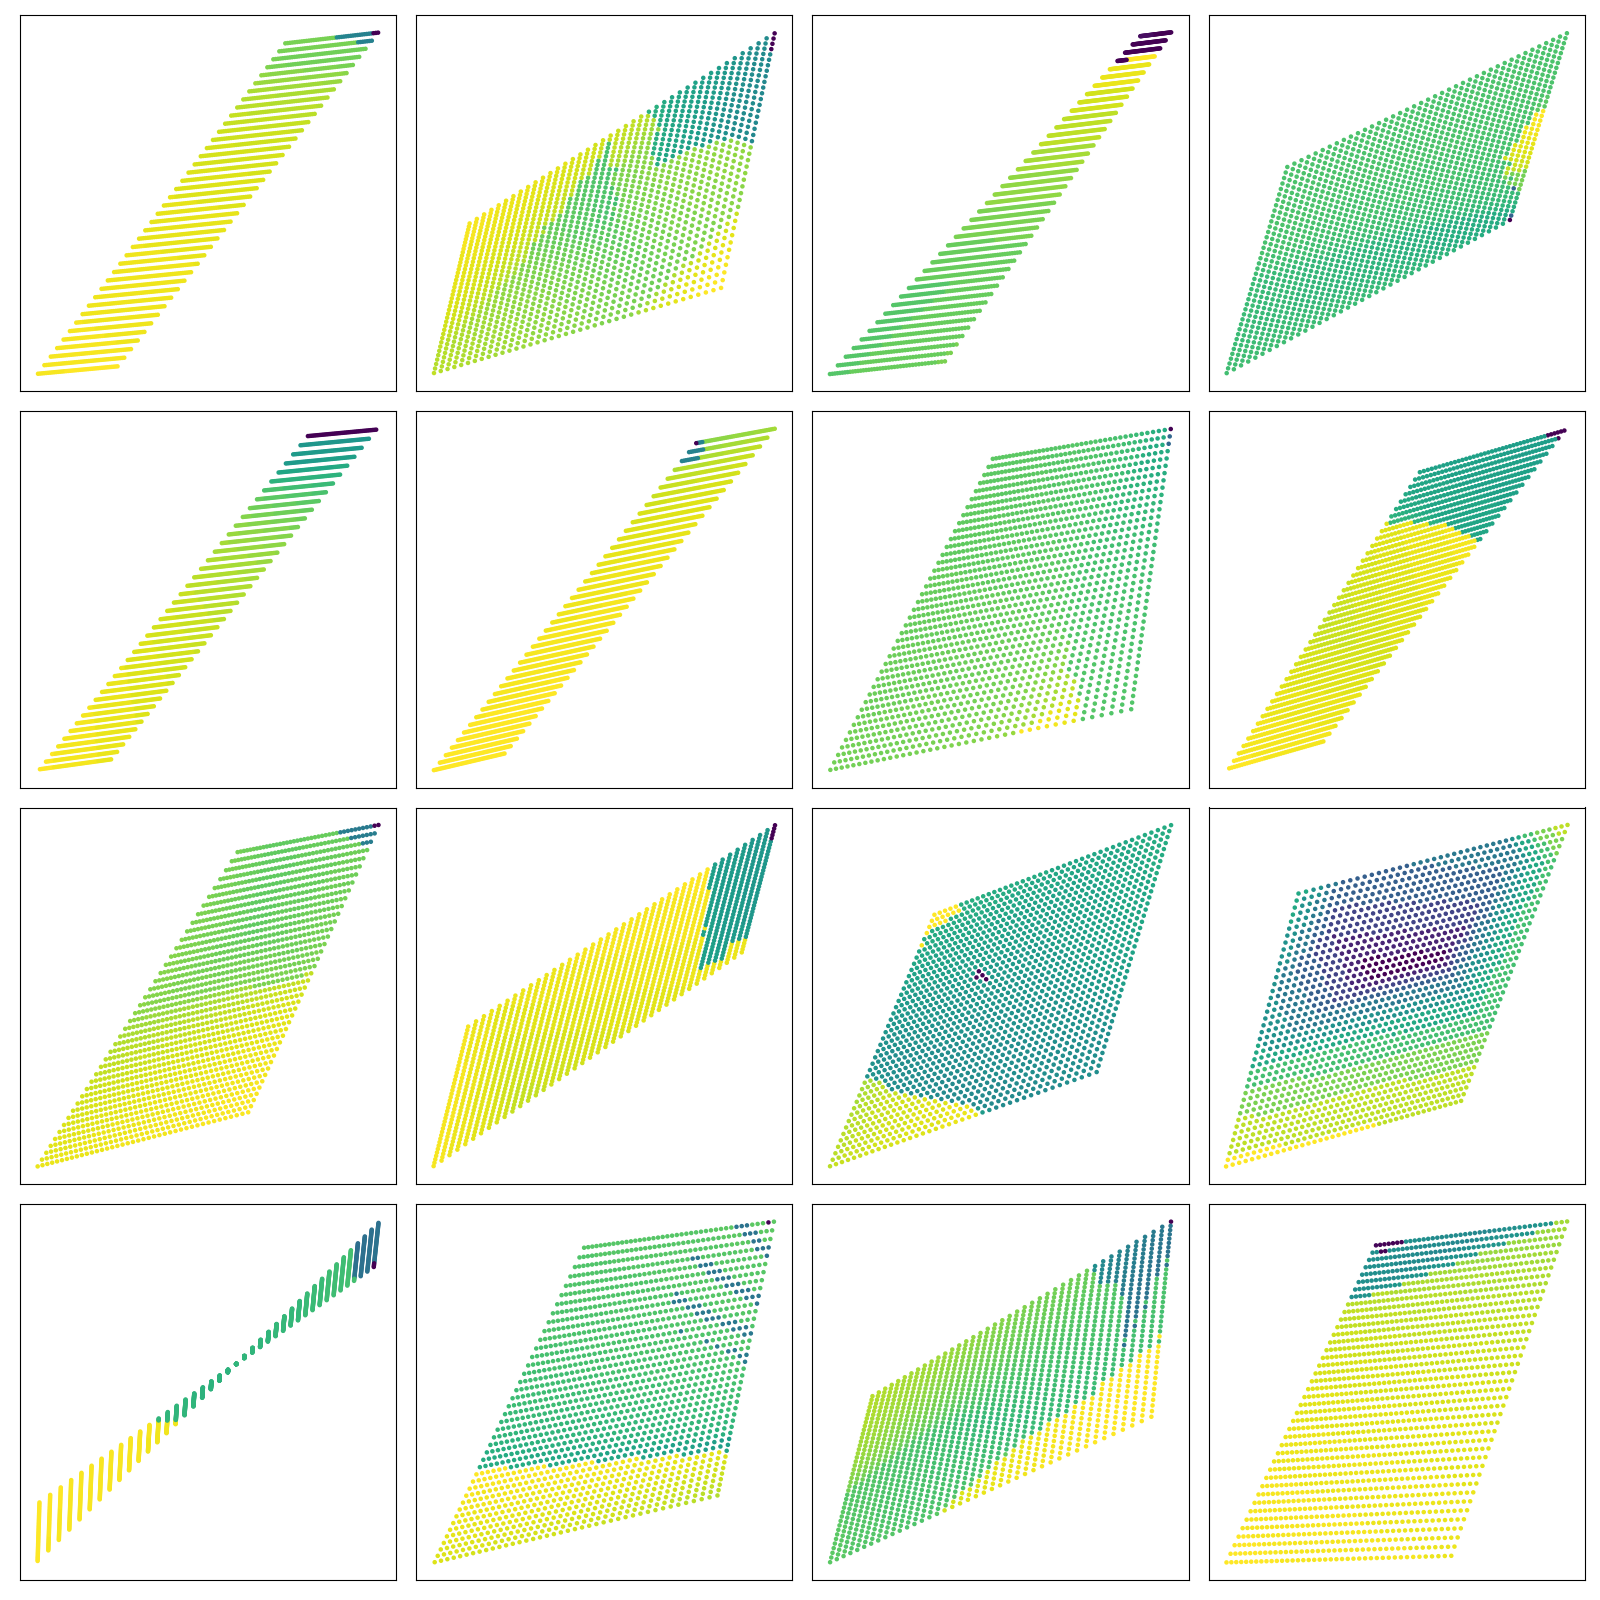
\includegraphics[width=1\textwidth,height=1\textheight]{../../pictures/figures/mvi-iterations.png}
% \caption{Above you see: various MDPs where the value of each policy is colored
% by the number of iterations it took to converge to the optimum policy. Yellow is many iterations, purple is few iterations.}
% \end{figure}


% {\color{red}TODO. need to include some plots of vanilla PG}

\subsection{Overparameterisation}

Recently there has been work investigating the properties of overparameterised search spaces.
Arora et al. 2018 \cite{Arora2018} prove that overparameterisation yields acceleration, however,
their explanation of the acceleration is not entirely convincing (as it requires first order assumptions).

More applied to RL, we want to know: how does overparameterisation effect the search for optimal policies?

In figures \ref{param-compare-sgd} and \ref{param-compare-sgd} we can see that
parameterisation can yield vastly different training trajectories\footnotemark to gradient descent,

\footnotetext{Is there are any advantages to certain types of trajectory?}

{\color{red}TODO regnerate ims and fix captions}

\begin{figure}
\centering
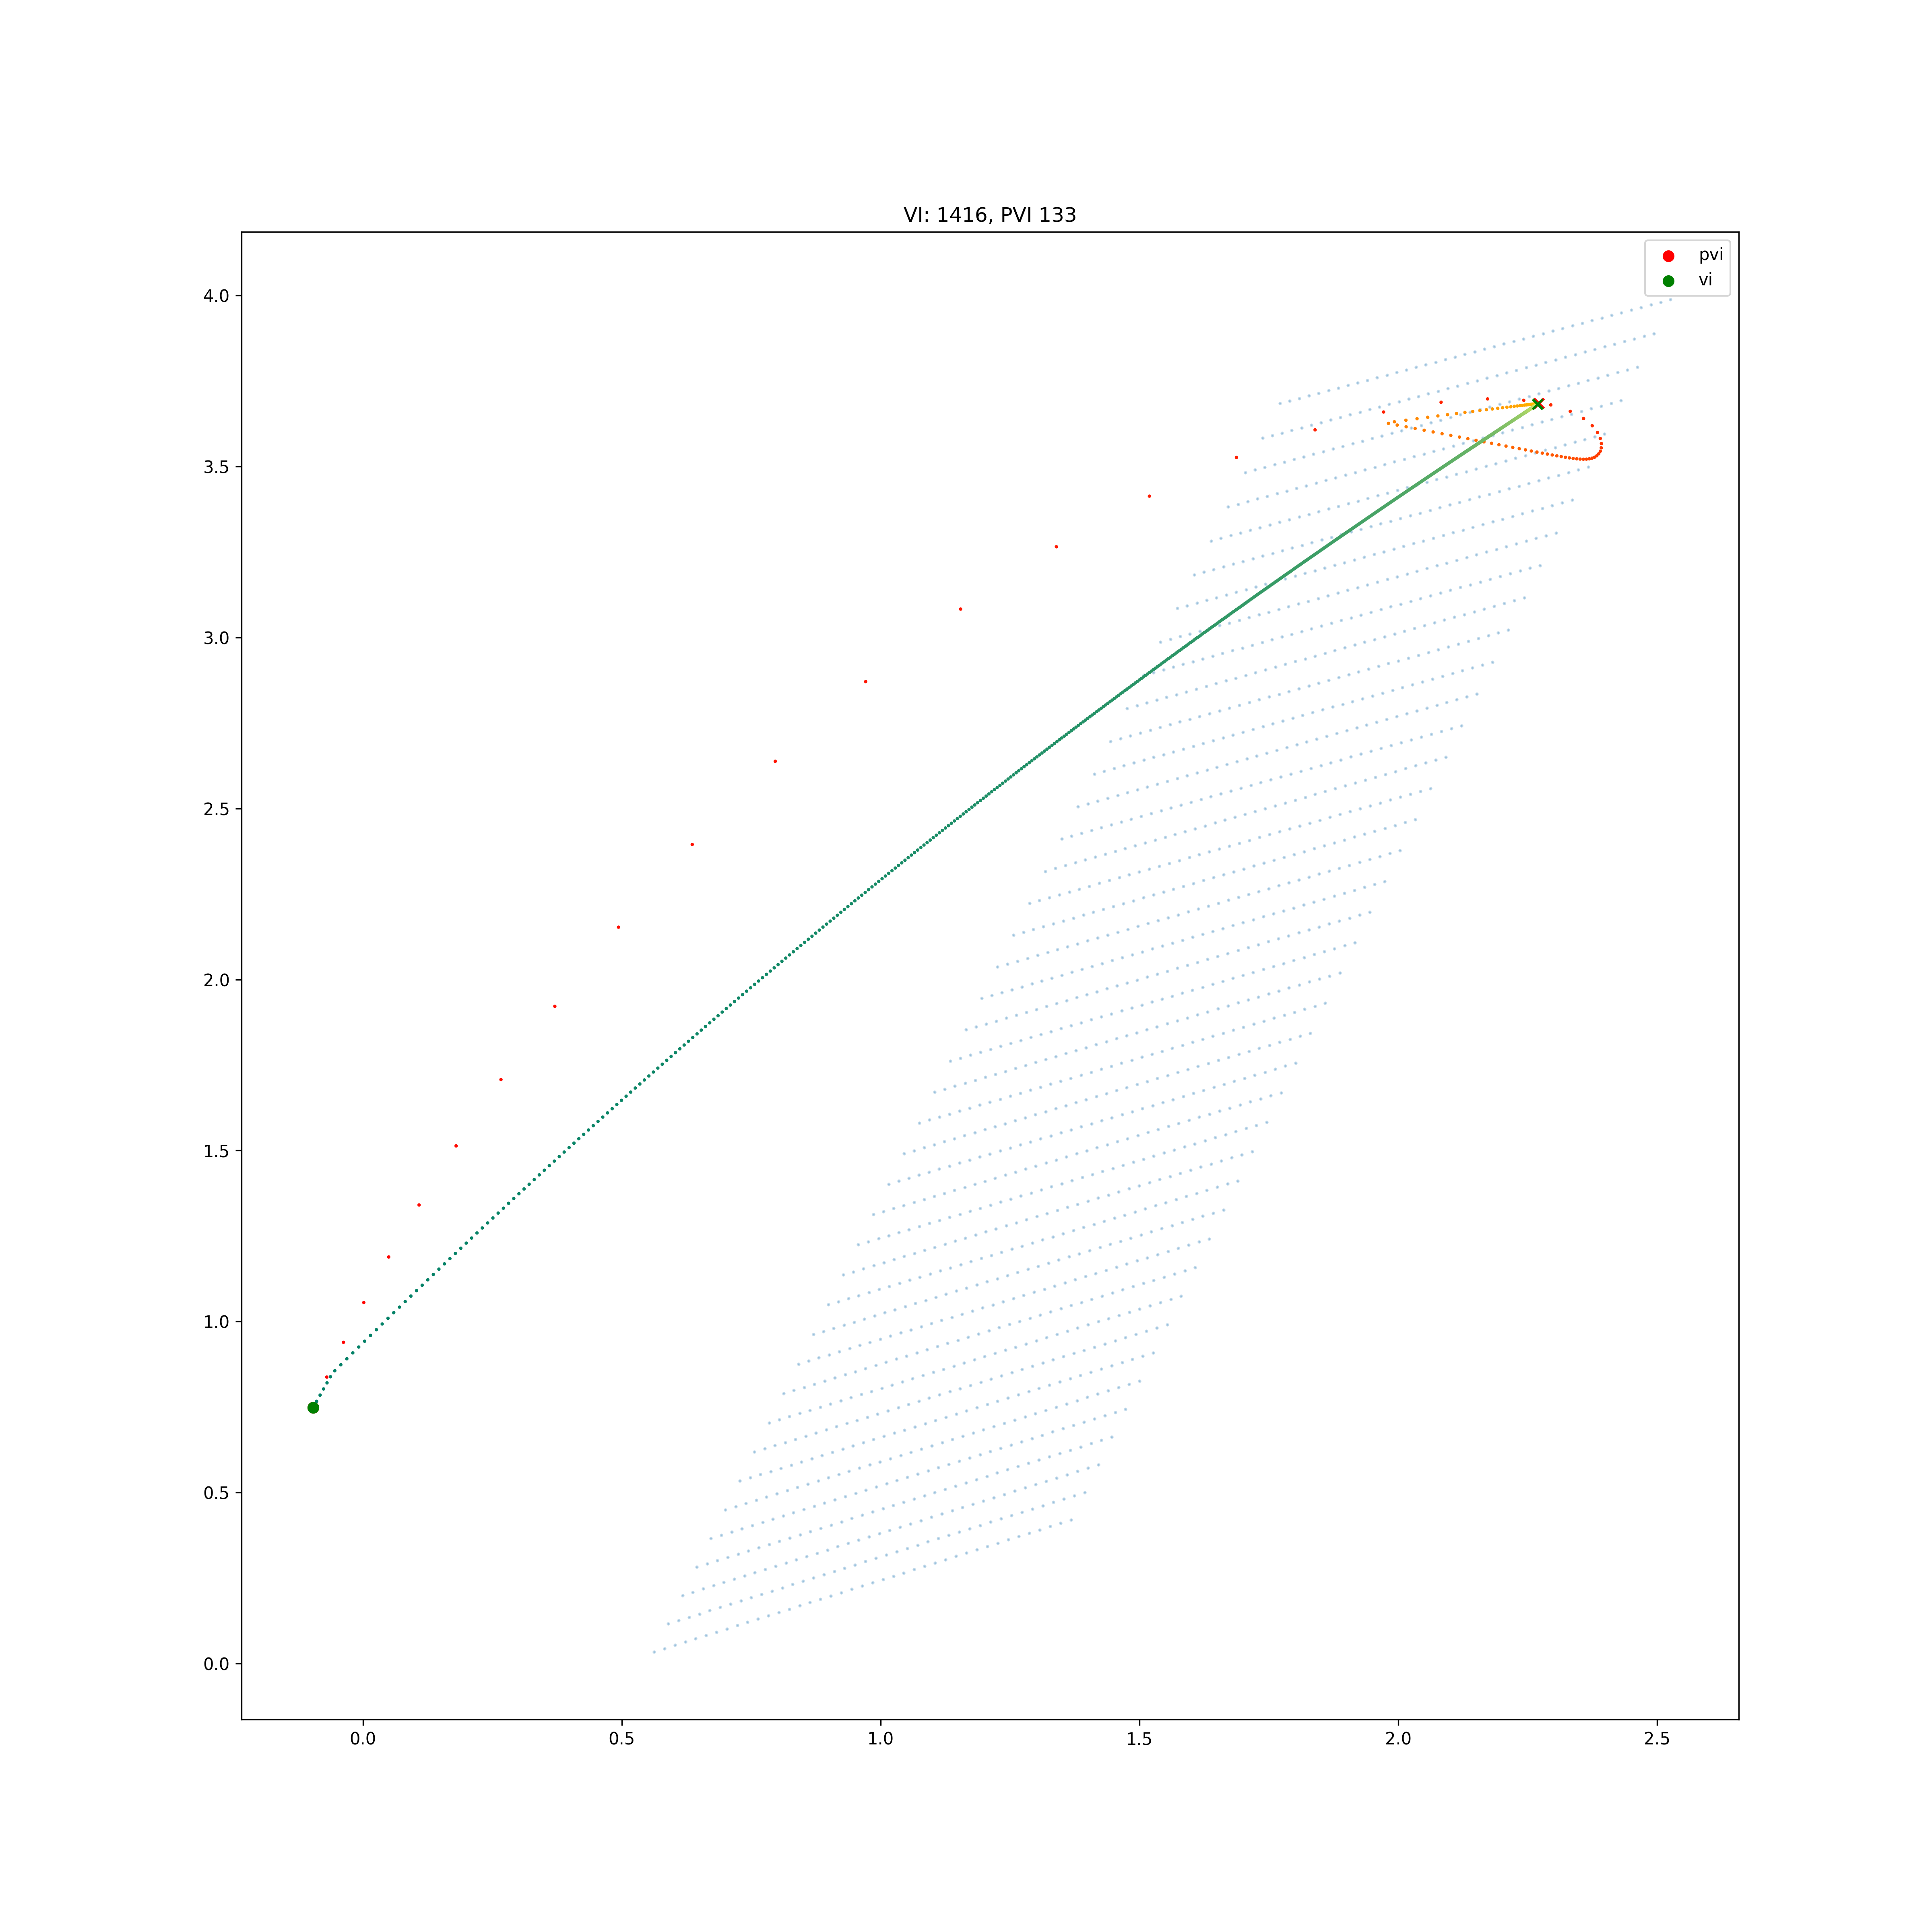
\includegraphics[width=1.0\textwidth,height=0.5\textheight]{../../pictures/figures/vi-vs-pvi.png}
\caption{The optimisation dynamics of value iteration versus parameterised value iteration.
Green is SGD's trajectory, and orange is }
\label{param-compare-sgd}
\end{figure}

\begin{figure}
\centering
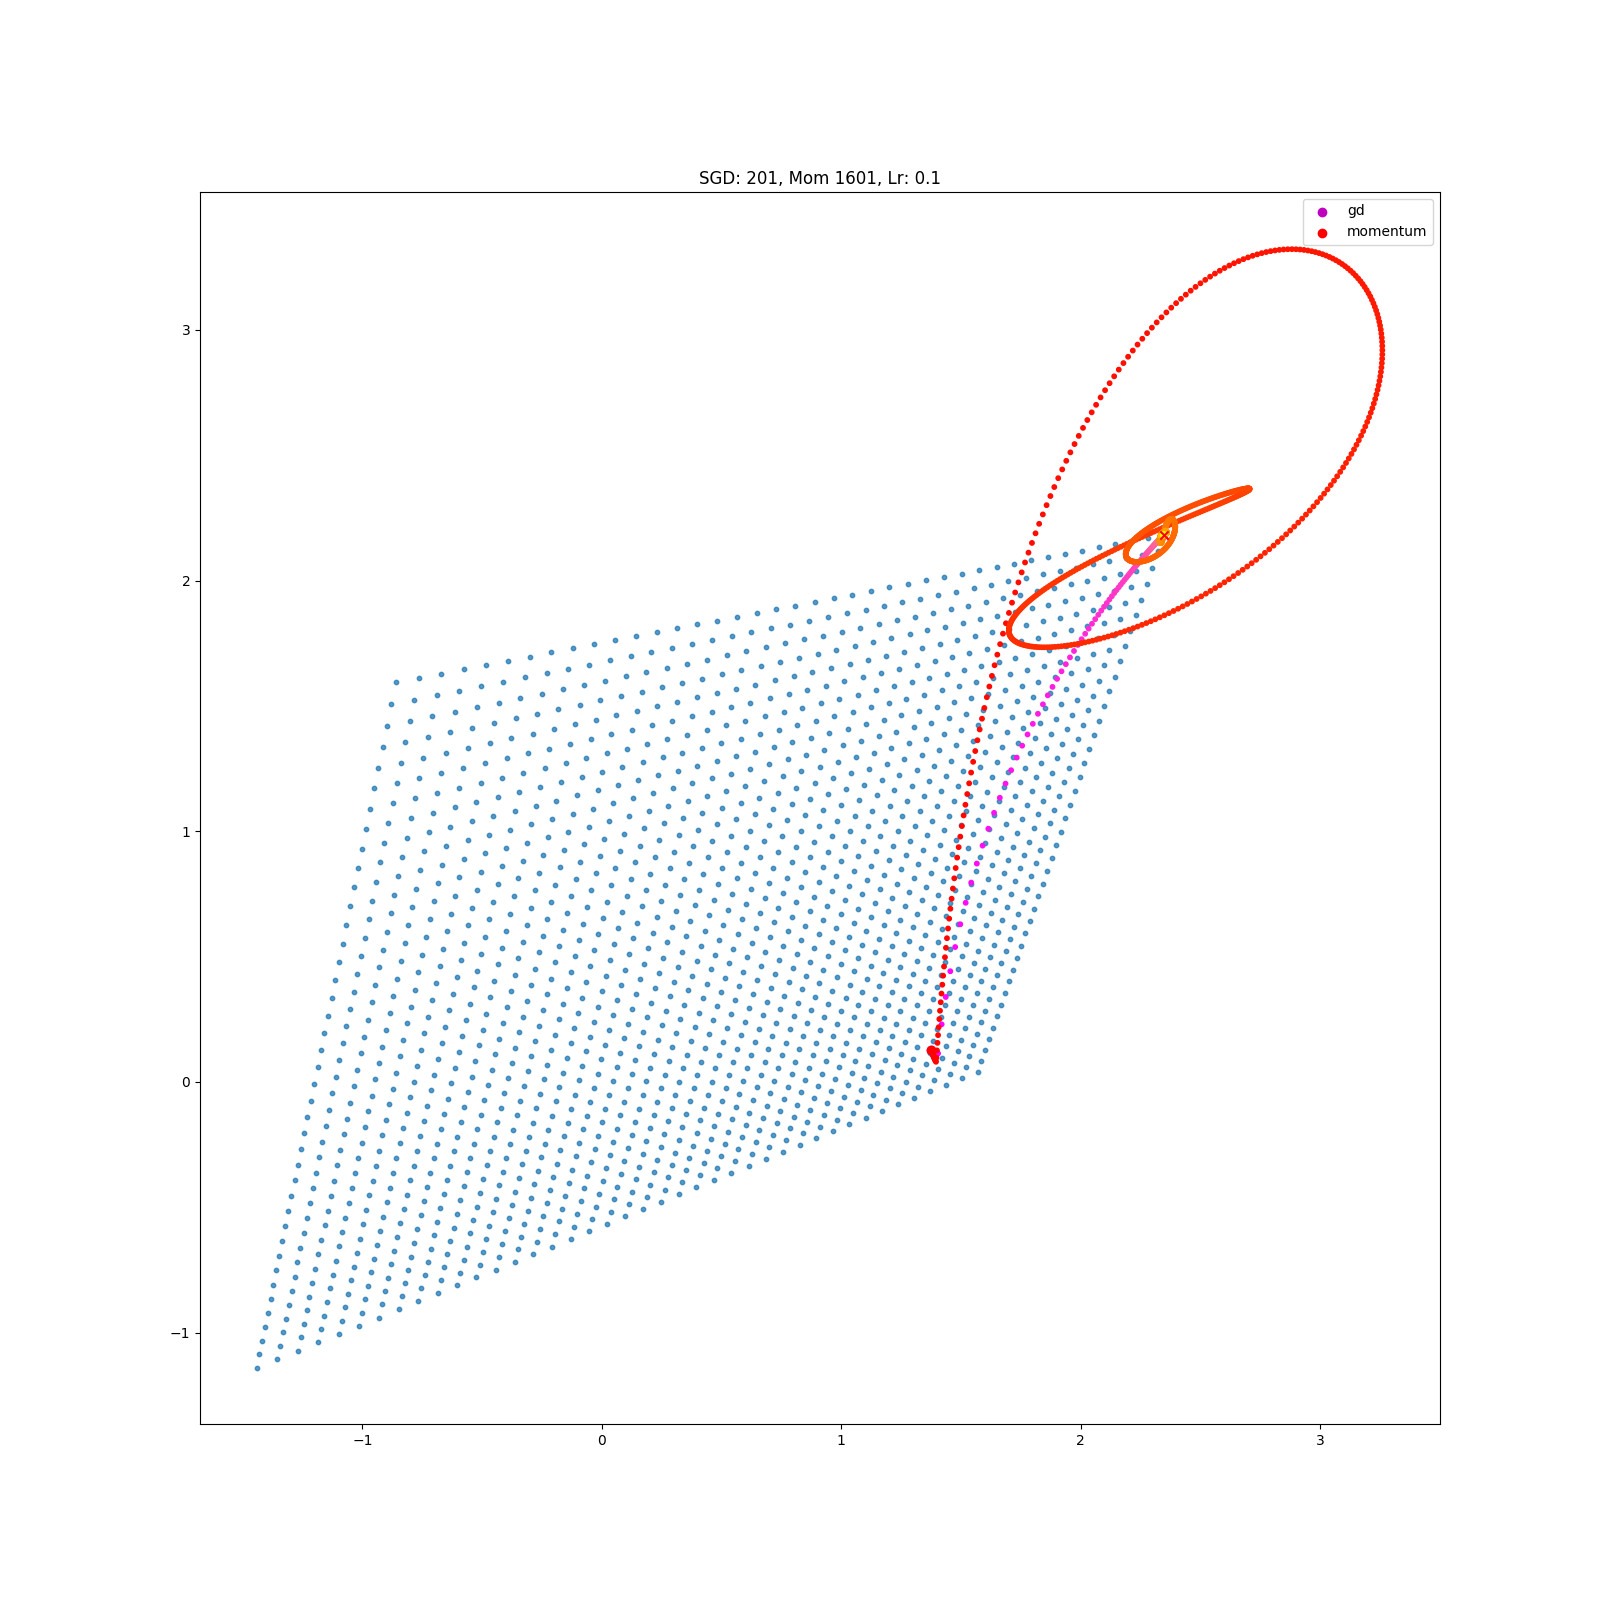
\includegraphics[width=1.0\textwidth,height=0.5\textheight]{../../pictures/figures/vi_sgd-vs-vi_mom_01.png}
\caption{The optimisation dynamics of value iteration versus value iteration with momentum.
Green is SGD's trajectory, and orange is momentum's trajectory.}
\label{mom-compare-sgd}
\end{figure}

In \ref{fig:iteration-complexity} we can observe that there can be sharp boundaries
between neighboring policies. A kind of phase transition, between the optimal policy being easy to find, and not.
(despite the fact that the we started from neighboring points).

\begin{figure}
\label{fig:iteration-complexity}
\centering
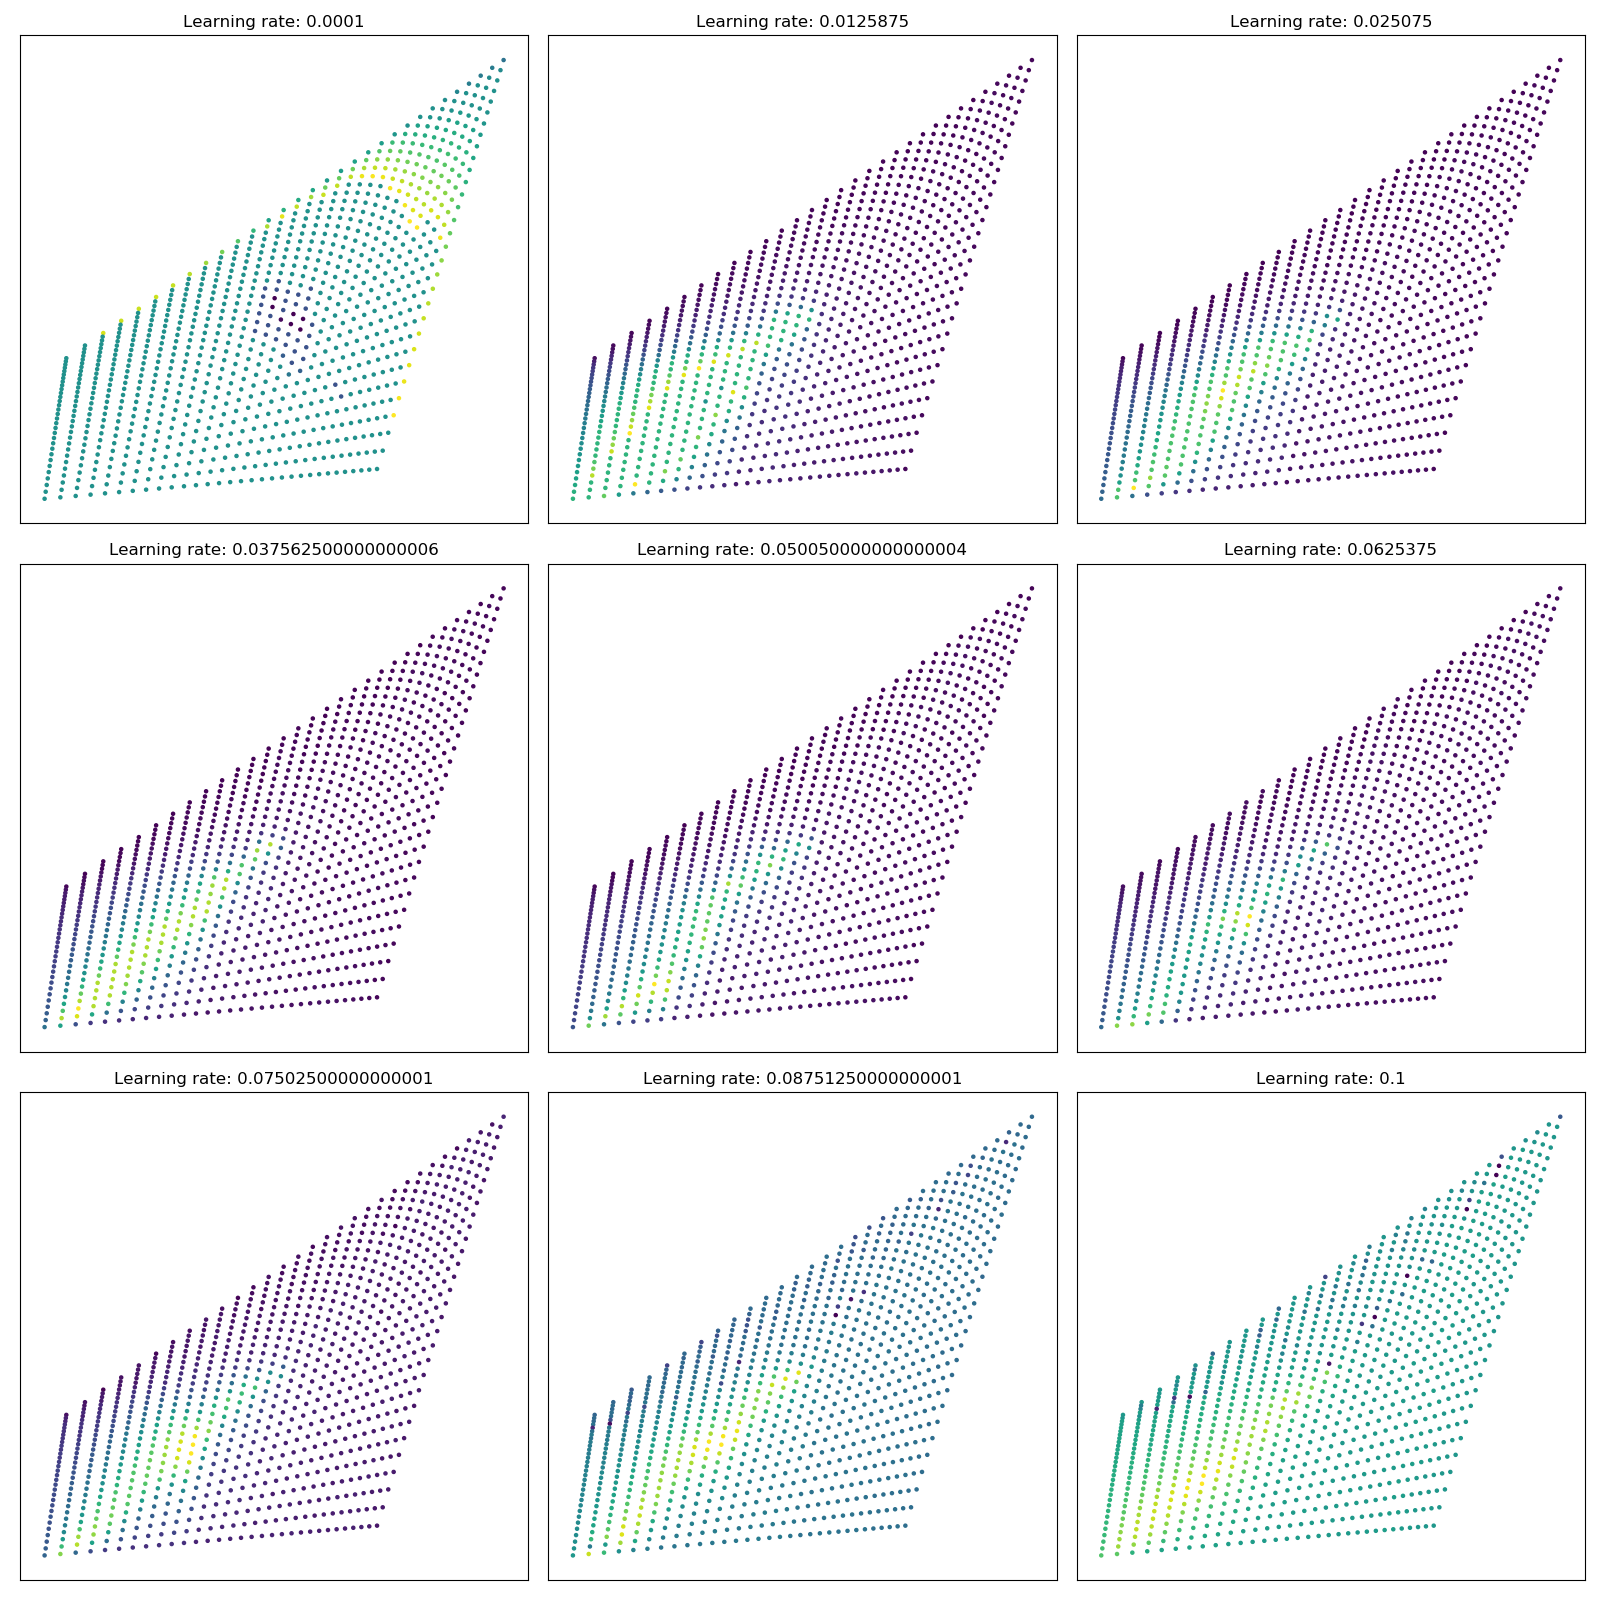
\includegraphics[width=1.0\textwidth,height=1.0\textheight]{../../pictures/figures/iteration-lr-0.png}
\caption{Here we have visualised the value polytope a 2-state, 2-action MDP.
These value polytopes are colored by the iteration complexity (many iterations - yellow, few iterations - purple) of parameterised policy gradients.
Each polytope was generated using a different learning rates.}
\end{figure}


% In which spaces can we get the most information? (e.g. low variance gradients)
% In which spaces to we have access to reliable guidance (e.g. large magnitude gradients)?
% SNR

% \cite{Brandfonbrener2019} consider the same setting, with an additional simplification. In the cts limit. No step sizes / learning rate.
% Obviously this simplification is not realistic. As in our experiments we see divergence with a overparameterised linear model.

% If we overparameterise the search space, then we can move between solutions in new ways. We can `tunnel' from A to B, without crossing C.
%  insert pic / prove
%
% Every point (in output space) is closer, when measured in the distance in parameter space needed to be traveled.
% insert pic / prove

\newpage
\subsection{Reparameterisation}

% Its effect on topology and acceleration.

{\color{red}Not sure if I should include this section. Very early stage...}

\begin{displayquote}
  \textsl{If we are allowed to arbitrarily pick our optimisation space, which should we pick?}
\end{displayquote}

Here we raise the question: should, and if so, how can, we rationally pick the
search space given knowledge of the loss function and likely starting points?

Consider the simple convex problem;

\begin{align*}
  x^{* } = \mathop{\text{argmin}}_{x} x^2
\end{align*}

We can pick some other space, $Z$, that we want to search in. And we can map $Z$ on to $X$ using $f: Z \to X$.

\begin{align*}
  z^{* } &=\mathop{\text{argmin}}_{z} f(z)^2 \\
    x^{* } &= f(z^{* })
\end{align*}

If we pick some simple functions for $f$. What happens? Well, if $f$ is non-linear
then we lose the guarantees convergence of convex search. However, what is gained?

\begin{figure}[h!]
\centering
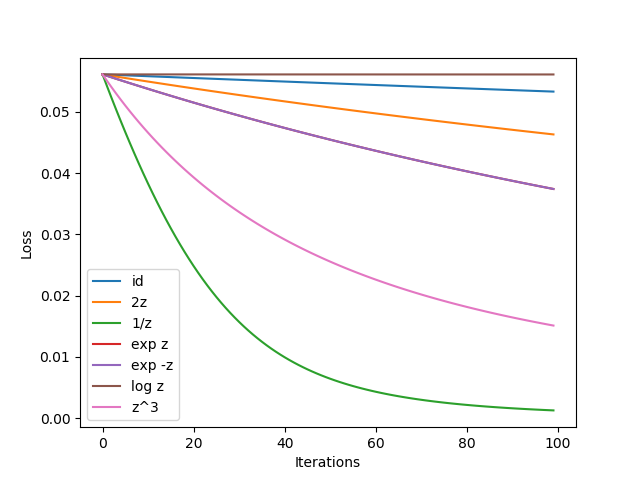
\includegraphics[width=0.7\textwidth,height=0.35\textheight]{../../pictures/figures/reparam-ce-04.png}
\caption{The iteration complexity of different initialisations and different learning rates.}
\end{figure}

\begin{figure}[h!]
\centering
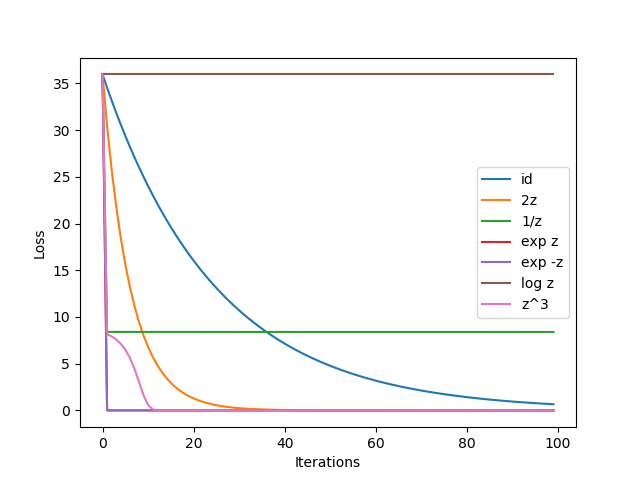
\includegraphics[width=0.7\textwidth,height=0.35\textheight]{../../pictures/figures/reparam-mse-04.png}
\caption{The iteration complexity of different initialisations and different learning rates.}
\end{figure}

When $z$ is the parameters of a deep neural network, the search space has certain properties: for example it's euclidean.
An alternative could be to search through a hyperbolic space, yielding 'hyperbolic neural networks' (explored by \ref{Ganea2018}).

\chapter{Abstraction}

\section{Similarity}

\subsection{Pairing abstractions with similarity measures}

% we have a similarity measure and a way to allow the learner to use it. now ...

Want to remove unimportant structure, while keeping the structure that allows us
to exploit the bellman equation (and thus more efficient search).

Different abstraction spaces support different similarity measures.
State similarity based on value fails in rather simple settings.
But works with state-action abstractions!?

Weaker notions of similarity.
\begin{itemize}
\tightlist
  \item Preserving the ordering of policies. Rather than their absolute value.
  \item Preserving ordering of value. $\phi(s) > \phi(s') \implies Q_{\pi}(s, a) > Q_{\pi}(s', a)$
  \item Preserving the neighbourhoods of policies and their values.
  \item ?
\end{itemize}


\section{LMDPs}

\subsection{LMDP solutions}\label{lmdp-derivation}

% Pick $a \in A$, versus, pick $\Delta(S)$. $f: S\to A$ vs $f:S \to \Delta(S)$.

In the original Todorov paper \cite{Todorov2009}, they derive the LMDP equations for minimising a cost function. This maximisation derivation just changes a few negative signs around.
% Although there is also a subtle change in the interpretation of what the unconstrained dynamics are doing. (??? explain)

\begin{align*}
V(s) &= \mathop{\text{max}}_{u} q(s) - \text{KL}(u(\cdot| s) \parallel p(\cdot | s)) + \gamma \mathop{\mathbb E}_{s' \sim u(\cdot | s)} V(s') \tag{1}\\
\\
&= q(s) + \mathop{\text{max}}_{u} \bigg[ \mathop{\mathbb E}_{s' \sim u(\cdot | s)} \log(\frac{p(s' | s) }{ u(s' | s)}+\gamma \mathop{\mathbb E}_{s' \sim u(\cdot | s)} \big[V(s')\big] \bigg] \tag{2}\\
\log(z_{u^{* }}(s)) &= q(s) + \mathop{\text{max}}_{u} \bigg[ \mathop{\mathbb E}_{s' \sim u(\cdot | s)} \log(\frac{p(s' | s) }{ u(s' | s)}+\mathop{\mathbb E}_{s' \sim u(\cdot | s)} \big[\log(z_{u^{* }}(s')^{\gamma})\big] \bigg] \tag{3}\\
&= q(s) + \mathop{\text{max}}_{u} \bigg[ \mathop{\mathbb E}_{s' \sim u(\cdot | s)} \log(\frac{p(s' | s)z_{u^{* }}(s')^{\gamma} }{ u(s' | s)} ) \bigg] \tag{4}\\
G(s) &= \sum_{s'} p(s' | s) z_{u^{* }}(s')^{\gamma} \tag{5}\\
&= q(s) + \mathop{\text{max}}_{u} \bigg[ \mathop{\mathbb E}_{s' \sim u(\cdot | s)} \log(\frac{p(s' | s)z_{u^{* }}(s')^{\gamma} }{ u(s' | s)} \cdot \frac{G(s)}{G(s)} ) \bigg] \tag{6}\\
&= q(s) + \log G(s) + \mathop{\text{min}}_{u} \bigg[\text{KL}\big(u(\cdot | s) \parallel \frac{p(\cdot | s)\cdot z_{u^{* }}(\cdot)^{\gamma}}{G(s)} \big) \bigg] \tag{7}\\
u^{* }(\cdot | s) &= \frac{p(\cdot | s)\cdot z_{u^{* }}(\cdot)^{\gamma}}{\sum_{s'} p(s' | s) z_{u^{* }}(s')^{\gamma}} \tag{8}\\
\log(z_{u^{* }}(s)) &= q(s) + \log \big(\sum_{s'} p(s' | s) z_{u^{* }}(s')^{\gamma}\big) \tag{9}\\
z_{u^{* }}(s) &= e^{q(s)}\big(\sum_{s'} p(s' | s) z_{u^{* }}(s')^{\gamma}\big) \tag{10}\\
z_{u^{* }} &= e^{q(s)}\cdot P z_{u^{* }}^{\gamma} \tag{11}\\
\end{align*}

By definition, an LMDP is the optimisation problem in (1). We can move the $\text{max}$ in (2), as $q(s)$ is not a function of $u$. Also in (2), expand the second term using the definition of KL divergence, the negative from the KL cancels the second terms negative. (3) Define a new variable, $z(s) = e^{v(s)}$. Also, use the log rule to move the discount rate. (4) Both expectations are under the same distribution, therefore they can be combined. Also, using log rules, combine the log terms. (5) Define a new variable that will be used to normalise $p(s' | s)z(s')^{\gamma}$. (6) Multiply and divide by $G(s)$. This allows us to rewrite the log term as a KL divergence as now we have two distributions, $u(\cdot | s)$ and $\frac{p(\cdot | s)z(\cdot)^{\gamma}}{G(s)}$. (7) The change to a KL term introduces a negative, instead of maximising the negative KL, we minimise the KL. Also in (7) the extra G(s) term can be moved outside of the expectation as it is not dependent in $s'$. (8) Set the optimal policy to minimise the KL distance term. (9) Since we picked the optimal control to be the form in (8), the KL divergence term is zero. (10) Move the log. (11) Rewrite the equations for the tabular setting, where $z$ is vector, and the uncontrolled dynamics are a matrix.

\subsection{MDP Linearisation}\label{mdp-Linearisation}

The ability to solve LMDPs is great, but it's only useful if we can map MDPs into LMDPs, solve them, and map the solution back.
Our goal here is to find a LMDP that has 'similar' structure to the original MDP we were given.\footnotemark[1]

\footnotetext[1]{This derivation is not the same as in Todorov. He sets $b_a \neq r, b_a = r - \sum P \log P$.}

\begin{align*}
\forall s, s' \in S, \forall a \in A, \exists u_a& \;\;\text{such that;} \tag{1}\\
P(s' | s, a) &= u_a(s'|s)p(s'|s) \tag{2}\\
r(s, a) &= q(s) - \text{KL}(P(\cdot | s, a) \parallel u_a(\cdot| s) ) \tag{3}\\
\\
r(s, a) &= q(s) - \text{KL}(P(\cdot | s, a)\parallel\frac{P(\cdot | s, a)}{p(\cdot|s)}) \tag{4}\\
r(s, a) &= q(s) - \sum_{s'}P(s' | s, a) \log(p(s'|s)) \tag{5}\\
\\
m_{s'}[s]&:= \log p(s' | s) \tag{6}\\
D_{as'}[s] &:= p(s'|s, a) \tag{7}\\
c_{s'}[s] &:= q[s] \mathbf 1 - m_{s'}[s] \;\;\text{such that} \;\; \sum_{s'} e^{m_{s'}[s]} = 1 \tag{8}\\
\\
r_a &= D_{as'} ( q \mathbf 1 - m_{s'}) \;\;\forall s \tag{9}\\
r_a &= D_{as'}c_{s'}  \;\;\forall s \tag{10}\\
c_{s'} &= r_aD_{as'}^{\dagger} \;\;\forall s\tag{11}\\
q &= \log \sum_{s'} e^{c_{s'}} \;\;\forall s\tag{12}\\
m_{s'} &= q - c_{s'} \;\;\forall s\tag{13}\\
\end{align*}

We want to pick $p, q$ such that the dynamics of every action in the original MDP can be represented with a control (2),
and every reward generated by an action, can be given by a combination of the
state rewards and the $\text{KL}$-divergence between the true dynamics and a control (3).
Combine (2), (3) to yield (4). Expand the definition of $\text{KL}$-divergence to get (5).
Now, we move to a tabular representation., where $m_{s'}[s]$ and $c_{s'}[s]$ are vectors, and
$D_{as'}[s]$ is a matrix, defined in (6), (7), (8). With these new definitions, we can rewrite equation (5)
as (9). The expectation can be moved to include $q$ because it sums to one.
Substitute equation (8) into (9) to get (10). Solve the linear equation in (11) to get the value of $c_{s'}$.
Use the value of $c_{s'}$ to calculate the state rewards and unconditioned dynamics by using equations (12), (13) and (6).

\section{Symmetry}

\subsection{Efficient inference using symmetries}\label{symmetry-inference}

\paragraph{Output coupling}

Mahajan et al. propose to use knowledge similarity to share couple outputs.
\cite{Mahajan2017}

\begin{align*}
\chi: (S\times A) \times (S\times A) \to [0, 1] \\
\mathcal L(\theta) = \mathop{\mathbb E}_{\chi} \Big[(Q(s, a, \theta)-Q(s', a', \theta))^2 \Big]
\end{align*}

Coupling the outputs of similar state-actions. This is nice because, we might know
that $s, a$ and $s', a'$ are similar. Yet we many not have observed $s', a'$.

% Equivalent to sharing training data?!?

However, how did we know that $s, a$ and $s', a'$ are similar without seeing $s', a'$?

- Data sharing (aka duplicate tuples \cite{Ho2019a})

\paragraph{Gradient coupling}

\begin{align*}
\nabla_{\theta} \ell(s, a, \theta) = \nabla_{\theta} \ell(s', a', \theta) \\
\chi \cdot \nabla_{\theta} \mathcal L(\theta)
\end{align*}

If $\chi$ has the structure $\chi((s, a), (s', a')) = \langle \nabla_{\theta}f(s, a, \theta), \nabla_{\theta} f(s', a', \theta) \rangle$ then will couple gradient in a certain way. NTK.

\cite{Ho2019a}

\paragraph{Data augmentation}

Sharing targets between 'similar' inputs.

\paragraph{Architecture}

Weight sharing?!? Weight coupling!?
\cite{Ravanbakhsh2017a,Abdolhosseini}
\cite{Anselmi2019}

\begin{center}\rule{0.5\linewidth}{\linethickness}\end{center}

\begin{displayquote}
\textit{Which method of incorporating knowledge of symmetries is best?}
\end{displayquote}

\begin{itemize}
\tightlist
  \item Data augmentation: flips.
  \item Gradient coupling: ??? gets complicated?
  \item Output coupling: regulariser on similar outputs.
  \item Architecture: mirror weights.
\end{itemize}

Equivalent?! (in this case, or in general?)
What other ways are there? Want to construct the space of possible ways to incorporate symmetries into a learner.


\subsection{Cart pole} \label{game-invariants}

\subsubsection{Mirror symmetry}

What are the invariants of the mirror cart pole example?

\begin{itemize}
	\tightlist
	\item the expected return is invariant to
	\item the Bellman residual is invariants to ...
	\item the reachable rewards are invariant to flips around the mirror plane
\end{itemize}
There is also an equivariant quantity, the change in state (assuming the representation of the state is equal to ...)


\begin{figure}[h!]
	\centering
	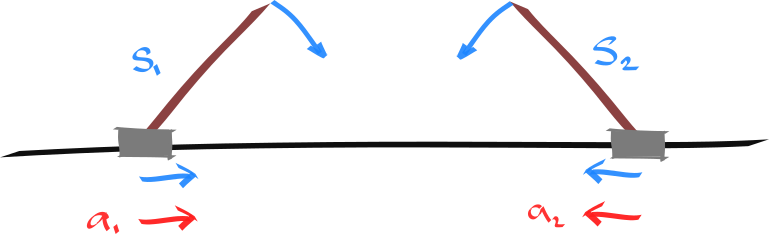
\includegraphics[width=1\textwidth,height=0.25\textheight]{../../pictures/drawings/cart-pole-mirror.png}
	\caption{Two mirror symmetric states of a cart pole.}
\end{figure}

Define the action of $f \in S_2$ on the;

\begin{itemize}
	\tightlist
	\item state space $f \circ s = -s$
	\item action space $f \circ a = -a$
 	\item policy to be $f \circ \pi(a | s) = \pi(f \circ a | f \circ s)$.
	\item transition function to be $(f \circ P)(\cdot | s, a) = P(\cdot| f \circ s, f \circ a)$. ???
\end{itemize}

Therefore, we can write $(f \circ Q^{\pi})(s, a) = Q^{f \circ \pi}(f \circ s, f \circ a)$.
We can write the properties above as;

\begin{align*}
Q^\pi(s, a) &= (f \circ Q^{\pi})(s, a) \tag{expected return}\\
T(Q^\pi)(s,a) - Q^\pi(s,a) &=T(f \circ Q^\pi)(s, a) - (f \circ Q^\pi)(s,a) \tag{Bellman residual}\\
\mathop{\mathbb E}_{s' \sim P(\cdot| s, a)} (s' - s) &= f \circ \mathop{\mathbb E}_{s' \sim (f \circ P)(\cdot| s, a)} (s' - f \circ s) \tag{change in state}\\
\end{align*}
\footnotemark[14]

The rewards (/ value) reachable from $s_1$ are also reachable from $s_2$ (which also implies the converse).
\footnotetext[14]{Note, this assumes we have a 'nice' state representation where differences make sense}

{\color{red}TODO verify these invariants!?!?}

Is this combination of invariants unique to the mirror symmetry? (how to prove this?!)

\subsubsection{Translational symmetry}

What are the invariants of the translated cart pole example?

\begin{figure}[h!]
\centering
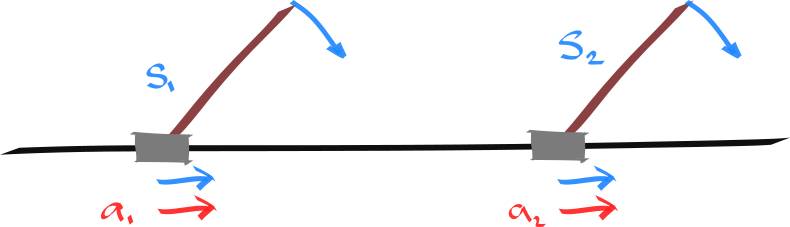
\includegraphics[width=1\textwidth,height=0.25\textheight]{../../pictures/drawings/cart-pole-translation.png}
\caption{Two similar cart poles, which are only a translation different from each other.}
\end{figure}

(special case of 'regular actions')

How to prove that this is a cts symmetry!?

Define the action of $g \in R$ on the;

\begin{itemize}
	\tightlist
	\item state space $g \circ s = g+s$
	\item action space $g \circ a = a$
 	\item policy to be $g \circ \pi(a | s) = \pi(a | g \circ s)$.
	\item transition function to be $(g \circ P)(\cdot | s, a) = P(\cdot| g \circ  s,  a)$. ???
	\item value function to be $(g \circ  Q^{\pi})(s, a) = Q^\pi(g \circ  s,  a)$
\end{itemize}

{\color{red}Huh, the key is the action. These have the same invariants!??!}

\begin{align}
Q^\pi(s, a) &= (g \circ Q^{\pi})(s, a) \tag{expected return}\\
T(Q^\pi)(s,a) - Q^\pi(s,a) &=T(g \circ Q^\pi)(s, a) - (g \circ Q^\pi)(s,a) \tag{Bellman residual}\\
\mathop{\mathbb E}_{s' \sim P(\cdot| s, a)} (s' - s) &= f \circ \mathop{\mathbb E}_{s' \sim (f \circ P)(\cdot| s, a)} (s' - f \circ s) \tag{change in state}\\
\end{align}

\subsubsection{Future translational symmetry}

\begin{figure}[!h]
\centering
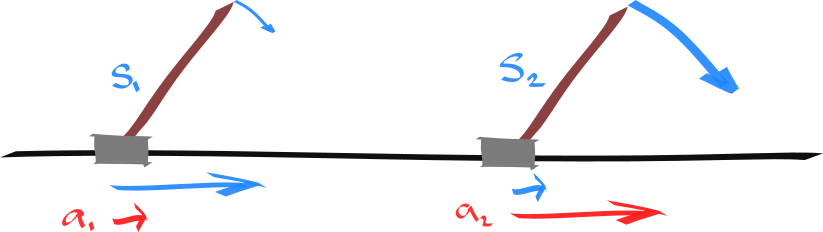
\includegraphics[width=1\textwidth,height=0.25\textheight]{../../pictures/drawings/cart-pole-state.png}
\caption{???}
\end{figure}

Different states, different actions, result in the same next state.
(ahh. $Q$ values are not equivalent if we are have a reward function that punishes larger actions!)

\begin{itemize}
\tightlist
  \item the state space to be $h\circ s = ??$ (related to lagrange transform / permutation!? conservation of momentum?!)
  \item the action space to be $h\circ a = ??$
  \item the transition function to be $h\circ P(\cdot|s, a) = P(\cdot|h \circ s, h \circ a)$
  \item the reward function to be $(h \circ r)(s, a) = $
  \item the value function to be $(h\circ Q)(s, a) = (h \circ r)(s, a) + \gamma \mathop{\mathbb E}_{s' \sim (h\circ P)(\cdot|s, a)} V(s')$
\end{itemize}

This implies. $Q(s, a) = $


\subsubsection{Temporal symmetry}

{\color{red} this one seems hard. not sure i am going to be able to explicitly construct this one?!}


\begin{figure}[!h]
\centering
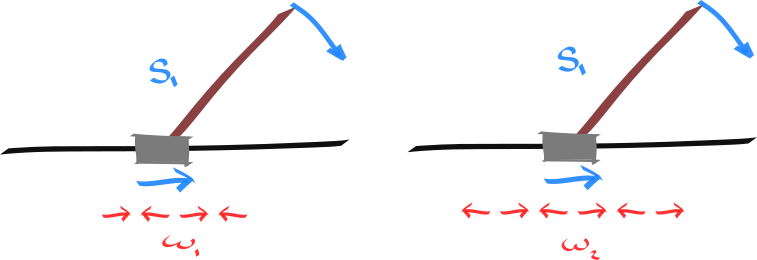
\includegraphics[width=1\textwidth,height=0.25\textheight]{../../pictures/drawings/cart-pole-temporal-approx.png}
\caption{???}
\end{figure}

\begin{align}
p(\cdot|s_1, \omega_1) = p(\cdot|s_1, \omega_2) \\
Q_{\pi}(s_1, \omega_1) = Q_{\pi}(s_1,\omega_2) \\
\end{align}


\subsection{Pong}

\subsubsection{Mirror symmetry (vertical)}

{\color{red}Need to be more careful with the state / action spaces here. Need to define properly!?}

\begin{figure}[!h]
\centering
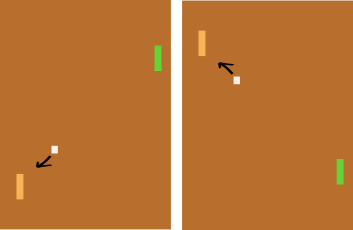
\includegraphics[width=1\textwidth,height=0.25\textheight]{../../pictures/drawings/pong-vert-flip.png}
\caption{???}
\end{figure}


Define the action of $f \in S_2$ on the;

\begin{itemize}
	\tightlist
	\item state space $f \circ s = I(x, -y)$
	\item action space $f \circ a = -a$
 	\item policy to be $f \circ \pi(a | s) = \pi(f \circ a | f \circ s)$.
	\item transition function to be $(f \circ P)(\cdot | s, a) = P(\cdot| f \circ s, f \circ a)$. ???
	\item value function to be $(f \circ Q^{\pi})(s, a) = Q^{f \circ \pi}(f \circ s, f \circ a)$
\end{itemize}

\begin{align}
\Delta_{T}(s, a) = (T \circ Q)(s,a) - Q(s,a)\\
\Delta_{T}(s_1, a_1) = \Delta_{T}(s_2, a_2) \\
\end{align}

\begin{align}
\forall a \text{ set}\;\;\pi(a | s_1) = \pi(-a| s_2) \\
Q_\pi(s_1, a_1) = Q_\pi(s_2, a_2) \\
Q_\pi(s_1, a_2) = Q_\pi(s_2, a_1) \\
\end{align}

\hypertarget{mirror-symmetry-horizontal}{%
\paragraph{Mirror symmetry
(horizontal)}\label{mirror-symmetry-horizontal}}

\begin{figure}
\centering
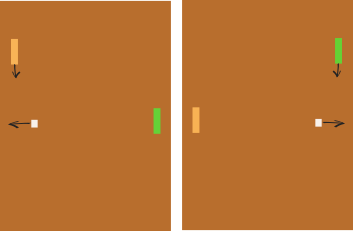
\includegraphics[width=1\textwidth,height=0.25\textheight]{../../pictures/drawings/pong-horz-flip.png}
\caption{???}
\end{figure}

Upon pretending to play as your opponent (flipping the image and
inverting the colors, via \(\rho: O \to O\), and ??? the actions)

\begin{align}
Q(s_1, a_1) = - V(\rho(s_2)) \\
\end{align}

(\emph{this really requires you to disentangle the model from your
opponent!?})

\begin{align}
\tau(s'|s, a_{p=0}) &= f_{p=0}(s''|s, a) \cdot f_{p=1}(s'|s'', \hat a) \cdot \pi_{p=1}(\hat a|s'') \\
Q_{p=0}(s, a) &= -Q_{p=1}(s, a)
\end{align}

\hypertarget{translational-symmetry-1}{%
\paragraph{Translational symmetry}\label{translational-symmetry-1}}

\begin{figure}
\centering
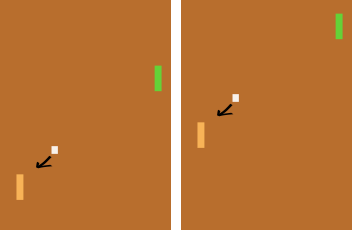
\includegraphics[width=1\textwidth,height=0.25\textheight]{../../pictures/drawings/pong-trans.png}
\caption{???}
\end{figure}

(\emph{although there are boundary cases which cannot be ignored. how
can they be dealt with!?})

\begin{align}
\forall a: Q_{\pi_1}(s_1, a) = Q_{\pi_2}(s_2, a) \\
\forall a, t: \pi_1(a|s^t_{s^0=s_1}) = \pi_2(a|s^t_{s^0=s_2})
\end{align}

If we take the same actions, in translated states, we get the same
outcome (up to the boundary conditions).

\hypertarget{temporal-symmetries}{%
\paragraph{Temporal symmetries}\label{temporal-symmetries}}

\begin{figure}
\centering
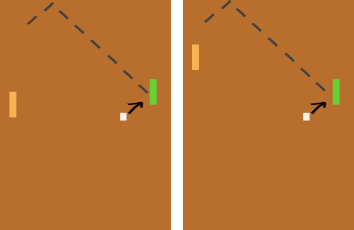
\includegraphics[width=1\textwidth,height=0.25\textheight]{../../pictures/drawings/pong-reach.png}
\caption{???}
\end{figure}

\begin{align}
\exists \pi_1, \pi_2 \;\;\text{s.t.} \;\; Q^{\pi_1}(s_1, a_1) = Q^{\pi_2}(s_2, a_2)
\end{align}

The same future state can be reached, and thus the same rewards can be
achieved.

\subsection{Rejection Sampling}\label{rejection-sampling}

\begin{algorithm}
	\caption{Rejection sampling}
	\begin{algorithmic}[1]

		\Procedure{RS}{$p, q, k$}
		\State $t=0$
		\While{not accepted}
			\State $x\sim U([0, 1])$
			\If{$x < \frac{p(x)}{kq(x)}$}
				\State $Break$
			\EndIf
			\State $t += 1$
		\EndWhile
		\State \algorithmicreturn{ $x$}
		\EndProcedure

	\end{algorithmic}
\end{algorithm}


\end{document}
